% To optimize for digital output (this changes the color palette add the option: digitaloutput
% To use \ifnomenclature add the option nomenclature
% To use bibtex or biblatex - include one of these as an option
\documentclass[nomenclature, english, biblatex]{kththesis}

\ifbiblatex
    %\usepackage[language=english,bibstyle=authoryear,citestyle=authoryear, maxbibnames=99]{biblatex}
    \usepackage[style=numeric,sorting=none,backend=biber]{biblatex}
    % \usepackage[bibstyle=authoryear,citestyle=authoryear, maxbibnames=99,language=english]{biblatex}
    % alternatively you might use another style, such as IEEE and use citestyle=numeric-comp  to put multiple citations in a single pair of square brackets
    %\usepackage[style=ieee,citestyle=numeric-comp]{biblatex}
    \addbibresource{references.bib}
    %\DeclareLanguageMapping{norsk}{norwegian}
\else
    % The line(s) below are for BibTeX
    \bibliographystyle{bibstyle/myIEEEtran}
    %\bibliographystyle{apalike}
\fi
%%%%%%%%%%%%%%%%%%%%%%%%%%%%%% Packages %%%%%%%%%%%%%%%%%%%%%%%%%%%%%%
% The following is for use with the KTH cover when not using XeLaTeX or LuaLaTeX
\ifxeorlua\relax
\else
\usepackage[scaled]{helvet}
\fi

%% The following are needed for generating the DiVA page(s)
\usepackage[force-eol=true]{scontents}              %% Needed to save lang, abstract, and keywords
\usepackage{pgffor}                 %% includes the foreach loop

%% Basic packages

%% Links
\PassOptionsToPackage{hyphens}{url}\usepackage{xurl}                %% Support for breaking URLs

%% Colorize
%\usepackage{color}
\PassOptionsToPackage{dvipsnames, svgnames, table}{xcolor}
\usepackage{xcolor}

\usepackage[normalem]{ulem}
\usepackage{soul}
\usepackage{xspace}
\usepackage{braket}

% to support units and decimal aligned columns in tables
\usepackage[locale=US]{siunitx}

\usepackage{balance}
\usepackage{stmaryrd}
\usepackage{booktabs}
\usepackage{graphicx}	        %% Support for images
\usepackage{multirow}	        %% Support for multirow columns in tables
\usepackage{tabularx}		    %% For simple table stretching
\usepackage{mathtools}
\usepackage{algorithm} 
\usepackage{algorithmic}  
\usepackage{amsmath}
\usepackage[linesnumbered,ruled,vlined,algo2e]{algorithm2e}
% can't use both algpseudocode and algorithmic packages
%\usepackage[noend]{algpseudocode}
%\usepackage{subfig}  %% cannot use both subcaption and subfig packages
\usepackage{subcaption}
\usepackage{optidef}
\usepackage{float}		        %% Support for more flexible floating box positioning
\usepackage{pifont}

%% some additional useful packages
% to enable rotated figures
\usepackage{rotating}	    	%% For text rotating
\usepackage{array}		        %% For table wrapping
\usepackage{mdwlist}            %% various list-related commands
\usepackage{setspace}           %% For fine-grained control over line spacing


\usepackage{enumitem}           %% to allow changes to the margins of descriptions


%% If you are going to include source code (or code snippets)
% \usepackage{listings}		    %% For source code listing
% \usepackage[cache=false]{minted} %% For source code highlighting
\usepackage{minted} %% For source code highlighting

\usepackage{bytefield}          %% For packet drawings


\setlength {\marginparwidth }{2cm} %leave some extra space for todo notes
\usepackage{todonotes}
\usepackage{notoccite} % do not number captions based on their appearance in the TOC


% Footnotes
\usepackage{perpage}
\usepackage[perpage,para,symbol]{footmisc} %% use symbols to ``number'' footnotes and reset which symbol is used first on each page


%% Various useful packages
%%----------------------------------------------------------------------------
%%   pcap2tex stuff
%%----------------------------------------------------------------------------
\usepackage{tikz}
\usepackage{colortbl}
\usetikzlibrary{arrows,decorations.pathmorphing,backgrounds,fit,positioning,calc,shapes}
\usepackage{pgfmath}	% --math engine
\newcommand\bmmax{2}
\usepackage{bm} % bold math


%% Managing titles
% \usepackage[outermarks]{titlesec}
%%%%%%%%%%%%%%%%%%%%%%%%%%%%%%%%%%%%%%%%%%%%%%%%%%%%%%%%%%%%%%%%%%%%%%
%\captionsetup[subfloat]{listofformat=parens}

% to include PDF pages
%\usepackage{pdfpages}


\usepackage{csquotes}               %% Recommended by biblatex
% to provide a float barrier use:
\usepackage{placeins}

\usepackage{comment}  %% Provides a comment environment
\usepackage{refcount}   %% to be able to get an expandable \getpagerefnumber

% for experiments with new cover
\usepackage{eso-pic}
\usepackage[absolute,overlay]{textpos}

% when the package is used, it draws boxes on the page showing the text, footnote, header, and margin regions of the page
%\usepackage{showframe}  
%\usepackage{printlen} % defines the printlength command to print out values of latex variable

\usepackage{xparse}  % to use for commands with optional arguments

\ifnomenclature
\usepackage[nocfg]{nomencl}  %% include refpage, refeq, to have page number and equation number for each nomenclature
\fi

\usepackage{longtable}  % For multipage tables
\usepackage{lscape}     % For landscape pages
\usepackage{needspace}  % to specify needed space, for example to keep listing heading with the listing
\usepackage{metalogo}   % for \XeLaTeX and \LuaLaTeX logos

%%% Local Variables:
%%% mode: latex
%%% TeX-master: t
%%% End:
% KTH colors for LaTeX documents
%
% Started from kthcolors by:
% Riccardo Sven Risuleo
% 2016-09-06 11:05:40
%
% from https://github.com/KTH-AC/kthcolors
%
% Adapted using the colors from "Graphic Profile Manual KTH" version 180604
% (i.e.. 2018-06-04) 
% see https://intra.kth.se/en/administration/kommunikation/grafiskprofil/kth-s-grafiska-profil-1.844676
% 
% G. Q. Maguire Jr.
% 2021-07-05
%

%\NeedsTexFormat{LaTeX2e}[1994/06/01]
%\ProvidesPackage{kthcolors}[2021/07/85 v3 Latex package with official KTH colors]

\RequirePackage{xcolor}
%% Primary colors
%% As of the new manual, there is only 1 primary color; but with three 
\definecolor{kth-blue}{RGB/cmyk}{25,84,166/0.849,0.494,0,0.349}
\colorlet{kth-blue80}{kth-blue!80!}
\colorlet{kth-blue40}{kth-blue!40!}

% these are no longer used as of 2018-06-04
%\definecolor{kth-red}{RGB/cmyk}{157,16,45/0,0.898,0.713,0.384}
%\definecolor{kth-green}{RGB/cmyk}{98,146,46/0.329,0,0.685,0.427}

%% Secondary colors
\definecolor{kth-lightblue}{RGB/cmyk}{36,160,216/0.833,0.259,0,0.153}
\colorlet{kth-lightblue80}{kth-lightblue!80!}
\colorlet{kth-lightblue40}{kth-lightblue!40!}

%\definecolor{kth-lightred}{RGB/cmyk}{228,54,62/0,0.763,0.728,0.106}
\definecolor{kth-lightred}{RGB}{216,84,151}
\colorlet{kth-lightred80}{kth-lightred!80!}
\colorlet{kth-lightred40}{kth-lightred!40!}

\definecolor{kth-lightgreen}{RGB/cmyk}{176,201,43/0.124,0,0.786,0.212} % olive
\colorlet{kth-lightgreen80}{kth-lightgreen!80!}
\colorlet{kth-lightgreen40}{kth-lightgreen!40!}

% Cool Gray 9C
%\definecolor{kth-coolgray}{RGB}{101,101,108}

% Cool Gray 10 suggested by Martin Krzywinski (see http://mkweb.bcgsc.ca/colorblind) 
\definecolor{kth-coolgray}{RGB}{99,102,106}
\colorlet{kth-coolgray80}{kth-coolgray!80!}
\colorlet{kth-coolgray40}{kth-coolgray!40!}

% Tertiary colors (yet more colors)
% All of these are no longer used
%\definecolor{kth-pink}{RGB/cmyk}{216,84,151/10,0.611,0.301,0.153}
%\definecolor{kth-yellow}{RGB/cmyk}{250,185,25/0,0.26,0.9,0.0196}
%\definecolor{kth-darkgray}{RGB/cmyk}{101,101,108/0.0648,0.0648,0,0.576}
%\definecolor{kth-middlegray}{RGB/cmyk}{189,188,188/0,0.00529,0.00529,0.259}
%\definecolor{kth-lightgray}{RGB/cmyk}{227,229,227/0.00873,0,0.00873,0.102}

%\DeclareOption{gray}{\colorlet{gray}{kth-darkgray}}

% These versions are designed to meet accessability requirements for digital media
% Note that the palette is more limited than for the print version of the colors
\ifdigitaloutput
    % primary color
    \definecolor{kth-blue}{HTML}{1954A6} % Deep sea
    \definecolor{kth-blue80}{HTML}{5E87C0}

    % Secondary colors
    \definecolor{kth-lightblue}{HTML}{2191C4} % Stratosphere
    \definecolor{kth-lightred}{HTML}{D02F80} % Fluorescence
    \definecolor{kth-lightred80}{HTML}{D95599}
    \definecolor{kth-lightgreen}{HTML}{62922E} % Front-lawn
    \definecolor{kth-coolgray}{HTML}{65656C} % Office
    \definecolor{kth-coolgray80}{HTML}{848489}
\fi



%\glsdisablehyper
%\makeglossaries
%\makenoidxglossaries
%%%% Local Variables:
%%% mode: latex
%%% TeX-master: t
%%% End:
\setabbreviationstyle[acronym]{long-short}
% The form of the entries in this file is \newacronym{label}{acronym}{phrase}
%                                      or \newacronym[options]{label}{acronym}{phrase}
% see "User Manual for glossaries.sty" for the  details about the options, one example is shown below
% note the specification of the long form plural in the line below

\newacronym{HRI}{HRI}{Human-Robot Interaction}
\newacronym{HHI}{HHI}{Human-Human Interaction}
\newacronym{MBTI}{MBTI}{Myers–Briggs Type Indicator}
\newacronym{NLP}{NLP}{Natural Language Processing}
\newacronym{NLU}{NLU}{Natural Language Understanding}
\newacronym{ML}{ML}{Machine Learning}
\newacronym{AI}{AI}{Artificial Intelligence}
\newacronym{LLM}{LLM}{Large Language Model}
\newacronym{GAN}{GAN}{Generative Adversarial Network}
\newacronym{CV}{CV}{Computer Vision}
\newacronym{STRAP}{STRAP}{Style Transfer via Paraphrasing}
\newacronym{TIPI}{TIPI}{Ten Item Personality Inventory}
\newacronym{ANOVA}{ANOVA}{Analysis of Variance}

\newacronym[longplural={Debugging Information Entities}]{DIE}{DIE}{Debugging Information Entity}
%
% The following example also uses options
\newacronym[plural={OSes}, firstplural={operating systems (OSes)}]{OS}{OS}{operating system}

% note the use of a non-breaking dash in long text for the following acronym
\newacronym{IQL}{IQL}{Independent Q‑Learning}

\newacronym{KTH}{KTH}{KTH Royal Institute of Technology}

\newacronym{TTS}{TTS}{Text-to-Speech}
\newacronym{LAN}{LAN}{Local Area Network}
% note the use of a non-breaking dash in the following acronym
\newacronym{WiFi}{Wi-Fi}{Wireless Fidelity}

\newacronym{WLAN}{WLAN}{Wireless Local Area Network}
\newacronym{UN}{UN}{United Nations}
\newacronym{SDG}{SDG}{Sustainable Development Goal}
                %load the acronyms file

\makeatletter
\newcommand{\DeclareLatinAbbrev}[2]{%
  \DeclareRobustCommand{#1}{%
    \@ifnextchar{.}{\textit{#2}}{%
      \@ifnextchar{,}{\textit{#2.}}{%
        \@ifnextchar{!}{\textit{#2.}}{%
          \@ifnextchar{?}{\textit{#2.}}{%
            \@ifnextchar{)}{\textit{#2.}}{%
              {\textit{#2.,\ }}}}}}}}%
}
\makeatother
\DeclareLatinAbbrev{\eg}{e.g}
\DeclareLatinAbbrev{\Eg}{E.g}
\DeclareLatinAbbrev{\ie}{i.e}
\DeclareLatinAbbrev{\Ie}{I.e}
\DeclareLatinAbbrev{\etc}{etc}
\DeclareLatinAbbrev{\etal}{et~al}

\def\first {$(i)$\xspace}
\def\second{$(ii)$\xspace}
\def\third {$(iii)$\xspace}
\def\fourth{$(iv)$\xspace}
\def\fifth {$(v)$\xspace}
\def\sixth {$(vi)$\xspace}
\def\seventh{$(vii)$\xspace}
\def\eighth{$(viii)$\xspace}

%%% custom definitions
%% Coloring the links!
\newcommand\myshade{75} % Usage: red!\myshade!black

\definecolor{ForestGreen} {RGB}{34,  139,  34}
\definecolor{HeraldRed2}   {rgb}{0.81, 0.12, 0.15}

\newcommand{\refscolor} {blue}
\newcommand{\linkscolor}{HeraldRed2}
\newcommand{\urlscolor} {ForestGreen}

%% Some definitions of used colors
%\definecolor{darkblue}{rgb}{0.0,0.0,0.3} %% define a color called darkblue
%\definecolor{darkred}{rgb}{0.4,0.0,0.0}
%\definecolor{red}{rgb}{0.7,0.0,0.0}
%\definecolor{lightgrey}{rgb}{0.8,0.8,0.8} 
%\definecolor{grey}{rgb}{0.6,0.6,0.6}
%\definecolor{darkgrey}{rgb}{0.4,0.4,0.4}
%\definecolor{aqua}{rgb}{0.0, 1.0, 1.0}

% For runin headings
\newcommand{\smartparagraph}[1]{\vspace{.05in}\noindent\textbf{#1}}

%% Table of Contents (ToC) depth 
\setcounter{secnumdepth}{4} % how many sectioning levels to assign numbers to
\setcounter{tocdepth}{4}    % how many sectioning levels to show in ToC

%% Limit hyphenation
\hyphenpenalty=9000
\tolerance=5000
% Reduce hyphenation as much as possible:
%\hyphenpenalty=15000
%\tolerance=1000

% For notes by the authors to themselves
\newcommand*{\todoinline}[1]{\textcolor{red}{TODO: #1}}

  % load some additional definitions to make writing more consistent

% The following is needed in conjunction with generating the DiVA data with abstracts and keywords using the scontents package and a modified listings environment
\ExplSyntaxOn
\newcommand\typestoredx[2]{\expandafter\__scontents_typestored_internal:nn\expandafter{#1} {#2}}
\ExplSyntaxOff
\makeatletter

%% definition of new command for bytefield package
\newcommand{\colorbitbox}[3]{%
	\rlap{\bitbox{#2}{\color{#1}\rule{\width}{\height}}}%
	\bitbox{#2}{#3}}

%% Acronyms
% note that nonumberlist - removes the cross references to the pages where the acronym appears
% note that super will set the descriptions text aligned
% note that nomain - does not produce a main glossary, thus only acronyms will be in the glossary
% note that nopoFot - will prevent there being a period at the end of each entry
\usepackage[acronym, style=super, section=section, nonumberlist, nomain, nopostdot]{glossaries}
\setlength{\glsdescwidth}{0.75\textwidth}
\usepackage[automake]{glossaries-extra}
\ifinswedish
    %\usepackage{glossaries-swedish}
\fi

% the tlg, tld, and dn will be the file extensions used for this glossary
\newglossary[tlg]{readme}{tld}{tdn}{README acronyms}
% define a left aligned table cell that is ragged right
\newcolumntype{L}[1]{>{\raggedright\let\newline\\\arraybackslash\hspace{0pt}}p{#1}}

% Because backref is not compatible with biblatex
\ifbiblatex
    \usepackage[plainpages=false]{hyperref}
\else
    \usepackage[
    backref=page,
    pagebackref=false,
    plainpages=false,
                            % PDF related options
    unicode=true,           % Unicode encoded PDF strings
    bookmarks=true,         % generate bookmarks in PDF files
    bookmarksopen=false,    % Do not automatically open the bookmarks in the PDF reading program
    pdfpagemode=UseNone,    % None, UseOutlines, UseThumbs, or FullScreen
    destlabel,              % better naming of destinations
    ]{hyperref}
    \usepackage{backref}
    %
    % Customize list of backreferences.
    % From https://tex.stackexchange.com/a/183735/1340
    \renewcommand*{\backref}[1]{}
    \renewcommand*{\backrefalt}[4]{%
    \ifcase #1%
          \or [Page~#2.]%
          \else [Pages~#2.]%
    \fi%
    }
\fi
\usepackage[all]{hypcap}	%% prevents an issue related to hyperref and caption linking


% packages that have to be included after hyperref
\usepackage{doi}
\usepackage[nameinlink]{cleveref}           %% Replace Section with a symbol


%\glsdisablehyper
\makeglossaries
%%% Local Variables:
%%% mode: latex
%%% TeX-master: t
%%% End:
\setabbreviationstyle[acronym]{long-short}
% The form of the entries in this file is \newacronym{label}{acronym}{phrase}
%                                      or \newacronym[options]{label}{acronym}{phrase}
% see "User Manual for glossaries.sty" for the  details about the options, one example is shown below
% note the specification of the long form plural in the line below

\newacronym{HRI}{HRI}{Human-Robot Interaction}
\newacronym{HHI}{HHI}{Human-Human Interaction}
\newacronym{MBTI}{MBTI}{Myers–Briggs Type Indicator}
\newacronym{NLP}{NLP}{Natural Language Processing}
\newacronym{NLU}{NLU}{Natural Language Understanding}
\newacronym{ML}{ML}{Machine Learning}
\newacronym{AI}{AI}{Artificial Intelligence}
\newacronym{LLM}{LLM}{Large Language Model}
\newacronym{GAN}{GAN}{Generative Adversarial Network}
\newacronym{CV}{CV}{Computer Vision}
\newacronym{STRAP}{STRAP}{Style Transfer via Paraphrasing}
\newacronym{TIPI}{TIPI}{Ten Item Personality Inventory}
\newacronym{ANOVA}{ANOVA}{Analysis of Variance}

\newacronym[longplural={Debugging Information Entities}]{DIE}{DIE}{Debugging Information Entity}
%
% The following example also uses options
\newacronym[plural={OSes}, firstplural={operating systems (OSes)}]{OS}{OS}{operating system}

% note the use of a non-breaking dash in long text for the following acronym
\newacronym{IQL}{IQL}{Independent Q‑Learning}

\newacronym{KTH}{KTH}{KTH Royal Institute of Technology}

\newacronym{TTS}{TTS}{Text-to-Speech}
\newacronym{LAN}{LAN}{Local Area Network}
% note the use of a non-breaking dash in the following acronym
\newacronym{WiFi}{Wi-Fi}{Wireless Fidelity}

\newacronym{WLAN}{WLAN}{Wireless Local Area Network}
\newacronym{UN}{UN}{United Nations}
\newacronym{SDG}{SDG}{Sustainable Development Goal}
                %load the acronyms file

% insert the configuration information with author(s), examiner, supervisor(s), ...
%% Information for inside title page


\authorsLastname{Galatolo}
\authorsFirstname{Alessio}
\email{galatolo@kth.se}
\kthid{galatolo}
% As per email from KTH Biblioteket on 2021-06-28 students cannot have an OrCiD reported for their degree project
\authorsSchool{\schoolAcronym{EECS}}
%If the student is not in Stockholm, Sweden, add that information here
% This information will be used when generating the acknowledgements signature.
%\authorCity{A City}
%\authorCountry{A Country}
% pass into \authorCityCountryDate{} the month and year for the acknowledgment
% If there is a second author and place, the month, and year are the same, the specify the month and year for the first author:
\authorCityCountryDate{\MONTH\enspace\the\year}
% if there is a second author and the place is different, then say:
%\authorCityCountryDate{}


\supervisorAsLastname{Winkle}
\supervisorAsFirstname{Katie}
\supervisorAsEmail{winkle@kth.se}
% If the supervisor is from within KTH add their KTHID, School and Department info
\supervisorAsKTHID{winkle}
\supervisorAsSchool{\schoolAcronym{EECS}}
\supervisorAsDepartment{Division of Robotics, Perception and Learning}
% other for a supervisor outside of KTH add their organization info
%\supervisorAsOrganization{Timbuktu University, Department of Pseudoscience}


\examinersLastname{Dos Santos Carvalho Leite}
\examinersFirstname{Iolanda}
\examinersEmail{iolanda@kth.se}
% If the examiner is from within KTH add their KTHID, School and Department info
\examinersKTHID{iolanda}
\examinersSchool{\schoolAcronym{EECS}}
\examinersDepartment{Division of Robotics, Perception and Learning}
% other for a examiner outside of KTH add their organization info
%\examinersOrganization{Timbuktu University, Department of Pseudoscience}

\date{\today}

\courseCycle{2}
\courseCode{DA233X}
\courseCredits{30.0}

\programcode{TMAIM}
\degreeName{Master of Science in Machine Learning}
% Note that the subject area for a Bachelor's thesis (Kandidatexamen) should be either Technology or Architecture
% If the thesis is in Swedish these would be: teknik | arkitektur   -- Note the use of lower case

\subjectArea{Computer Science and Engineering}

% if there is a second degree
%\secondProgramcode{CINTE}
%\secondDegreeName{test second degree}
%\secondSubjectArea{test second subject area}

% Note that in the case of both Both Degree of Master of Science in Engineering and Master's degree
% there are two cases: "Both" is used when the field of technology (\subjectArea{}) and the main subject (\secondSubjectArea{} are different and the case "Same" when they are the same.
%% Both case
%\courseCycle{2}
%\courseCode{xxxxxx}
%\courseCredits{30.0}
%\degreeName{Both Degree of Master of Science in Engineering and Master's degree}
%\subjectArea{Biotechnology}
%\secondSubjectArea{Medical Engineering}

%\courseCycle{2}
%\courseCode{xxxxxx}
%\courseCredits{30.0}
%\degreeName{Både civilingenjörsexamen och masterexamen}
%\subjectArea{bioteknik}
%\secondSubjectArea{medicinsk teknik}

%% Same case
%\courseCycle{2}
%\courseCode{xxxxxx}
%\courseCredits{30.0}
%\degreeName{Both Degree of Master of Science in Engineering and Master's degree}
%\subjectArea{Biotechnology}
%\secondSubjectArea{Biotechnology}

%\courseCycle{2}
%\courseCode{xxxxxx}
%\courseCredits{30.0}
%\degreeName{Både civilingenjörsexamen och masterexamen}
%\subjectArea{bioteknik}
%\secondSubjectArea{bioteknik}

% For a CDATE student the following are likely values:
%\programcode{CDATE}
%\courseCycle{2}
%\courseCode{DA231X}
%\courseCredits{30.0}
%\degreeName{Degree of Master of Science in Engineering}
%\subjectArea{Computer Science and Engineering}

% For a TCSCM student the following are likely values:
%\programcode{TCSCM}
%\courseCycle{2}
%\courseCode{DA231X}
%\courseCredits{30.0}
%\degreeName{Master's Programme, Computer Science, 120 credits}
%\subjectArea{Computer Science}

% For a CMETE student the following are likely values:
%\programcode{CMETE}
%\courseCycle{2}
%\courseCode{DA231X}
%\courseCredits{30.0}
%\degreeName{Degree of Master of Science in Engineering}
%\subjectArea{Media Technology}

% For a CINTE student the following are likely values:
%\programcode{CINTE}
%\courseCycle{2}
%\courseCode{DA231X}
%\courseCredits{30.0}
%\degreeName{Degree of Master of Science in Engineering}
%\subjectArea{Information and Communication Technology}


%%%%% for DiVA's National Subject Category information
%%% Enter one or more 3 or 5 digit codes
%%% See https://www.scb.se/contentassets/3a12f556522d4bdc887c4838a37c7ec7/standard-for-svensk-indelning--av-forskningsamnen-2011-uppdaterad-aug-2016.pdf
%%% See https://www.scb.se/contentassets/10054f2ef27c437884e8cde0d38b9cc4/oversattningsnyckel-forskningsamnen.pdf
%%%%
%%%% Some examples of these codes are shown below:
% 102 Data- och informationsvetenskap (Datateknik)    Computer and Information Sciences
% 10201 Datavetenskap (datalogi) Computer Sciences 
% 10202 Systemvetenskap, informationssystem och informatik (samhällsvetenskaplig inriktning under 50804)
% Information Systems (Social aspects to be 50804)
% 10203 Bioinformatik (beräkningsbiologi) (tillämpningar under 10610)
% Bioinformatics (Computational Biology) (applications to be 10610)
% 10204 Människa-datorinteraktion (interaktionsdesign) (Samhällsvetenskapliga aspekter under 50803) Human Computer Interaction (Social aspects to be 50803)
% 10205 Programvaruteknik Software Engineering
% 10206 Datorteknik Computer Engineering
% 10207 Datorseende och robotik (autonoma system) Computer Vision and Robotics (Autonomous Systems)
% 10208 Språkteknologi (språkvetenskaplig databehandling) Language Technology (Computational Linguistics)
% 10209 Medieteknik Media and Communication Technology
% 10299 Annan data- och informationsvetenskap Other Computer and Information Science
%%%
% 202 Elektroteknik och elektronik Electrical Engineering, Electronic Engineering, Information Engineering
% 20201 Robotteknik och automation Robotics
% 20202 Reglerteknik Control Engineering
% 20203 Kommunikationssystem Communication Systems
% 20204 Telekommunikation Telecommunications
% 20205 Signalbehandling Signal Processing
% 20206 Datorsystem Computer Systems
% 20207 Inbäddad systemteknik Embedded Systems
% 20299 Annan elektroteknik och elektronik Other Electrical Engineering, Electronic Engineering, Information Engineering
%% Example for a thesis in Computer Science and Computer Systems
\nationalsubjectcategories{10201, 10206}




\title{Towards Automatic Generation of Personality-Adapted Speech and Emotions for a Conversational Companion Robot}
\subtitle{}
\date{June 27, 2022}
% give the alternative title - i.e., if the thesis is in English, then give a Swedish title
\alttitle{Mot Automatisk Generering av Personlighets Anpassade Tal och Känslor för en Samtalskunnig Sällskaps Robot}
\altsubtitle{}

\EnglishKeywords{Personality, Emotions, Human-Robot Interaction, Machine Learning, Large Language Models, Text-style transfer, GPT-3, STRAP}
\SwedishKeywords{Personlighet, Känslor, Människa-robotinteraktion, Maskininlärning, Stora Språkmodeller, Överföring av text, GPT-3, STRAP}

%%%%% For the oral presentation
%% Add this information once your examiner has scheduled your oral presentation
\presentationDateAndTimeISO{2022-06-17 10:00}
\presentationLanguage{eng}
\presentationRoom{via Zoom https://kth-se.zoom.us/j/2507366330}
\presentationAddress{Room 406 (Teknikringen 14)}
\presentationCity{Stockholm}

% When there are multiple opponents, separate their names with '\&'
% Opponent's information
\opponentsNames{João Almeida}

% Once a thesis is approved by the examiner, add the TRITA number
% The TRITA number for a thesis consists of two parts a series (unique to each school)
% and the number in the series which is formatted as the year followed by a colon and
% then a unique series number for the thesis - starting with 1 each year.
\trita{TRITA-EECS-EX}{2022:00}

% Put the title, author, and keyword information into the PDF meta information
% This file contains the LaTeX to add information to the PDF file (specifically, author(s), title(s), and keywords
% It uses the hyperref package and should be be included before the \begin{document}
%
% I want to acknowledge the inspiration of Karl Voit's template for TU Graz that inspired me to add the PDF document information
% For more information about his template see https://github.com/novoid/LaTeX-KOMA-template
% Note that this template does not use anything from his template other than the names of the information for the PDF meta fields, i.e., mytitle, myauthor, and mykeywords together with the idea of defining the corresponding newcommand to set the relevant hyperref parameters.

\makeatletter
\ifx\@subtitle\@empty
    \newcommand{\mytitle}{\@title}
\else
    \newcommand{\mytitle}{\@title: \@subtitle}
\fi
\makeatother

\hypersetup{
     pdftitle={\mytitle}        % Title field
}

\makeatletter
\ifx\@secondAuthorsLastname\@empty
    \newcommand{\myauthor}{\@authorsFirstname\space\@authorsLastname} 
\else
    \ifinswedish
    \newcommand{\myauthor}{\@authorsFirstname\space\@authorsLastname\space\relax och\space\@secondAuthorsFirstname \@secondAuthorsLastname}
    \else
        \newcommand{\myauthor}{\@authorsFirstname\space\@authorsLastname\space\relax and\space\@secondAuthorsFirstname \@secondAuthorsLastname}
    \fi
\fi
\makeatother

\hypersetup{
     pdfauthor={\myauthor}      % Author field
}

% Put the alternative title (and subtitle) into the PDF Subject meta
\makeatletter
\ifx\@altsubtitle\@empty\relax
    \newcommand{\myalttitle}{\@alttitle}
\else
    \newcommand{\myalttitle}{\@alttitle: \@altsubtitle}
\fi
\makeatother

\hypersetup{
     pdfsubject={\myalttitle}        % Subject field
}

\makeatletter
\ifx\@EnglishKeywords\@empty
    \ifx\@SwedishKeywords\@empty
        \newcommand{\mykeywords}{}
    \else
    \newcommand{\mykeywords}{\@SwedishKeywords}
    \fi
\else
    \ifx\@SwedishKeywords\@empty
        \newcommand{\mykeywords}{\@EnglishKeywords}
    \else
        \ifinswedish
            \newcommand{\mykeywords}{\@SwedishKeywords, \@EnglishKeywords}
        \else
            \newcommand{\mykeywords}{\@EnglishKeywords, \@SwedishKeywords}
        \fi
    \fi
\fi
\makeatother

\hypersetup{
     pdfkeywords={\mykeywords}        % Keywords field
}        
% I have _not_ set the following fields:
%    pdfcreator             % Creator field
%    pdfproducer            % Producer field
 


% the custom colors and the commands are defined in defines.tex    
\hypersetup{
	colorlinks  = true,
	breaklinks  = true,
	linkcolor   = \linkscolor,
	urlcolor    = \urlscolor,
	citecolor   = \refscolor,
	anchorcolor = black
}

\ifnomenclature
% The following lines make the page numbers and equations hrefs in the Nomenclature list
\renewcommand*{\pagedeclaration}[1]{\unskip, \dotfill\href{page.#1}{page\nobreakspace#1}}
% The following does not work correctly, as the name of the cross-reference is incorrect
%\renewcommand*{\eqdeclaration}[1]{, see equation\nobreakspace(\href{equation.#1}{#1})}

% You can also change the page heading for the nomenclature
\renewcommand{\nomname}{List of Symbols Used}

% You can even add customization text before the list
\renewcommand{\nompreamble}{The following symbols will be later used within the body of the thesis.}
\makenomenclature
\fi


% my includes
\usepackage{adjustbox}
\newcommand{\vmark}{\ding{51}}
\newcommand{\xmark}{\ding{55}}
\usepackage{emoji}
\usepackage{caption}
\usepackage{subcaption}
\usepackage{pgfplots}
\pgfplotsset{compat=1.18} 
\usepackage{tikz}
\usetikzlibrary{shapes,er,positioning}
\tikzstyle{arrow} = [thick,->,>=stealth]
\usepackage{ifluatex}
\ifluatex
  \usepackage{pdftexcmds}
  \makeatletter
  \let\pdfstrcmp\pdf@strcmp
  \let\pdffilemoddate\pdf@filemoddate
  \makeatother
\fi
\usepackage{svg}

\begin{document}
\selectlanguage{english}

%%% Set the numbering for the title page to a numbering series not in the preface or body
\pagenumbering{alph}
\kthcover
\titlepage
% document/book information page
\bookinfopage

% Frontmatter includes the abstracts and table-of-contents
\frontmatter
\setcounter{page}{1}
\begin{abstract}
% The first abstract should be in the language of the thesis.
% Abstract fungerar på svenska också.
  \markboth{\abstractname}{}
\begin{scontents}[store-env=lang]
eng
\end{scontents}
%%% The contents of the abstract (between the begin and end of scontents) will be saved in LaTeX format
%%% and output on the page(s) at the end of the thesis with information for DiVA facilitating the correct
%%% entry of the meta data for your thesis.
%%% These page(s) will be removed before the thesis is inserted into DiVA.
\begin{scontents}[store-env=abstracts,print-env=true]
Previous works in Human-Robot Interaction have demonstrated the positive potential benefit of designing highly anthropomorphic robots. This includes physical appearance but also whether they can express emotions, behave in a congruent manner, etc. This work wants to explore the creation of a robot that is able to express a given personality consistently throughout a dialogue while also manifesting congruent emotional expressions. 

Personality defines many aspects of the character of a person and it can influence how one speaks, behaves, reacts to events, etc. Here, we only focus our attention on language and on how it changes depending on one particular personality trait, the extraversion. To this end, we tested different language models to automate the process of generating language according to a particular personality. We also compared large language models such as GPT-3 to smaller ones, to analyse how size can correlate to performance in this task. 

We initially evaluated these methods through a fairly small user study in order to confirm the correct manipulation of personality in a text-only context. Results suggest that personality manipulation and how well it is understood highly depend on the context of a dialogue, with a more `personal' dialogue being more successful in manifesting personality. Also, the performance of GPT-3 is comparable to smaller models, specifically trained, with the main difference only given in the perceived fluency of the generations. 

We then conducted a follow-up study where we chose to use a robot that is capable of showing different facial expressions used to manifest different emotions, the Furhat robot. We integrated into the robot the generations from our language models together with an emotion classification method that is used to guide its facial expressions. Whilst the output of our models did trigger different emotional expressions, resulting in robots which differed both in their language and nonverbal behaviour, resultant perception of these robots' personality only approached significance ($p\sim0.08$). In this study, GPT-3 performed very similarly to much smaller models, with the difference in fluency also being much smaller than before. We did not see any particular change in the perception of the robots in terms of likeability nor uncanniness. 

\end{scontents}

\subsection*{Keywords}
\begin{scontents}[store-env=keywords,print-env=true]
\InsertKeywords{english}
\end{scontents}

\clearpage
\end{abstract}
\cleardoublepage
\babelpolyLangStart{swedish}
\begin{abstract}
    \markboth{\abstractname}{}
\begin{scontents}[store-env=lang]
swe
\end{scontents}
\begin{scontents}[store-env=abstracts,print-env=true]
Tidigare arbeten inom Människa-robotinteraktion har visat den positiva potentiella fördelen med att designa mycket antropomorfa robotar. Detta inkluderar fysiskt utseende men också huruvida de kan uttrycka känslor, bete sig på ett kongruent sätt, etc. Detta arbete vill utforska skapandet av en robot som kan uttrycka en given personlighet konsekvent under en dialog samtidigt som den manifesterar kongruenta känslomässiga uttryck.

Personlighet definierar många aspekter av en persons karaktär och den kan påverka hur man talar, beter sig, reagerar på händelser etc. Här fokuserar vi vår uppmärksamhet endast på språket och på hur det förändras beroende på ett särskilt personlighetsdrag, extraversion. För detta ändamål testade vi olika språkmodeller för att automatisera processen att skapa språk enligt en viss personlighet. Vi jämförde även stora språkmodeller som GPT-3 med mindre, för att analysera hur storlek kan relatera till prestanda i denna uppgift.

Vi utvärderade inledningsvis dessa metoder genom en mindre användarstudie för att bekräfta att personligheten kan manipuleras på rätt sätt i en textbaserad kontext. Resultaten tyder på att personlighetsmanipulation och hur väl den förstås i hög grad beror på sammanhanget i en dialog, där en mer `personlig' dialog är mer framgångsrik när det gäller att manifestera personlighet. Prestandan hos GPT-3 är också jämförbar med mindre modeller, specifikt tränade på en uppgift, där den största skillnaden var i den genererade textens upplevda flyt.

Vi gjorde sedan en uppföljningsstudie där vi valde att använda en robot som är kapabel att visa olika ansiktsuttryck och därigenom kapabel att manifestera olika känslor, Furhat-roboten. Vi integrerade talet som genererades från våra språkmodeller i roboten tillsammans med en känsloklassificeringsmetod som används för att styra dess ansiktsuttryck. Medan resultatet av våra modeller framkallade olika känslomässiga uttryck, vilket resulterade i robotar som skilde sig åt både i språk och icke-verbal kommunikation, närmade sig endast den resulterande uppfattningen av dessa robotars personlighet signifikans ($p\sim0.08$). I denna studie presterade GPT-3 mycket likartat med mycket mindre modeller, med skillnaden i flyt också mycket mindre än tidigare. Vi såg ingen speciell förändring i uppfattningen av robotarna när det gäller sympati eller obehaglighet.


\end{scontents}
\subsection*{Nyckelord}
\begin{scontents}[store-env=keywords,print-env=true]
% SwedishKeywords were set earlier, hence we can use alternative 2
\InsertKeywords{swedish}
\end{scontents}
\end{abstract}
\babelpolyLangStop{swedish}

\cleardoublepage


\section*{Acknowledgements}
\markboth{Acknowledgements}{}
Throughout my journey at \gls{KTH}, there have been many people that have been helpful and that supported me all the way to my graduation.

I would first like to thank my supervisor, Katie Winkle, that has always been inspiring and helpful. She has guided me throughout the definition of this work's topic making me explore and understand my interests without ever limiting my thought process. Thanks to her, I was able to create the work of which I am most proud and that will end up positively influencing the years to come. I would also like to thank her for all the time she has spent giving me feedback that was always right and on-point.

I would also like to thank the Social Robotics group at \gls{KTH} and my examiner in particular, Iolanda Leite, for all the feedback and direction they have given me.

Next, I want to thank all of my family and my mother in particular for all the efforts made to support me in every choice I've made. Most of my journey would not have been possible without my mother's emotional and psychological support that she has always given me alongside all of her unconditional love.% and for always believing in me.

I would then like to thank all of my friends that have always been of great inspiration and guidance for my journey. For pushing me to always aim for the best I could achieve, even against big odds.

Finally, I cannot conclude this without mentioning my best friend and partner in life. Thanks to her I found the energy and motivation that I needed during my hardest times. Thanks to her I was able to expose myself and risk falling knowing she would always be there to catch me. She was especially supportive throughout the duration of this work, always listening to all of my blabberings and always showing interest even when listening to the same topic over and over.

\acknowlegmentssignature

\fancypagestyle{plain}{}
\renewcommand{\chaptermark}[1]{ \markboth{#1}{}} 
\tableofcontents
  \markboth{\contentsname}{}

\cleardoublepage
\listoffigures

\cleardoublepage

\listoftables
\cleardoublepage
% \lstlistoflistings\todo[inline, backgroundcolor=kth-lightgreen40]{If you have listings in your thesis. If not, then remove this preface page.}
\cleardoublepage
% Align the text expansion of the glossary entries
\newglossarystyle{mylong}{%
  \setglossarystyle{long}%
  \renewenvironment{theglossary}%
     {\begin{longtable}[l]{@{}p{\dimexpr 2cm-\tabcolsep}p{0.8\hsize}}}% <-- change the value here
     {\end{longtable}}%
 }
% \glsaddall
\printglossary[style=mylong, type=\acronymtype, title={List of acronyms and abbreviations}]

% if the nomenclature option was specified, then include the nomenclature page(s)
\ifnomenclature
    \cleardoublepage
    % Output the nomenclature list
    \printnomenclature
\fi

%% The following label is essential to know the page number of the last page of the preface
%% It is used to computer the data for the "For DIVA" pages
\label{pg:lastPageofPreface}
% Mainmatter is where the actual contents of the thesis goes
\mainmatter
\glsresetall
\renewcommand{\chaptermark}[1]{\markboth{#1}{}}
\selectlanguage{english}
\chapter{Introduction}
\label{ch:introduction}
\gls{HRI} is concerned with the study of how humans interact with robots. Among the many goals prefixed by this field, there is that of creating an interaction that is as natural as possible. Ways of achieving this range from making the robot's appearance more human-like as well as integrating different kinds of social intelligence into the robot. Having a more natural interaction can help in the perception of the robot in terms of how much the user likes it or how credible and persuasive it is considered~\cite{salem2012generation, salem2013err, sidner2004look, ullrich2017robot, aly2012robot, mobahi2003fuzzy}.

There have been multiple attempts at exploring the influence of integrating into a robot a personality~\cite{aly2013model, andriella2020have} or emotional capabilities~\cite{brianEmotions, desire, cozmoEmotions}. However, it is very rare to find a work that implements both extensively, with most of the studies that consider both only focusing on what (small) influence can personality have on the generated emotions~\cite{moshkina2011tame, han2012robotic}. Further, among the many ways to express personality e.g. body language, prosody, speech, etc. only a few have been explored and incorporated into robots. Many works focus only on body language~\cite{aly2013model, moshkina2011tame} while there is evidence in social sciences literature that personality has a significant influence on other aspects of life e.g. language~\cite{pennebaker1999linguistic, furnham1990language, thorne1987press, heylighen2002variation, dewaele1999extraversion}. Language is defined as the choice of words, their order and how they are used to formulate sentences in order to express a certain or multiple ideas. For example, a very extroverted person is generally more talkative and uses less complex sentences than an introverted one~\cite{pennebaker1999linguistic, furnham1990language}.

However, when integrating these social traits into robots, it is necessary to consider that both the robot's appearance and the inclusion of emotions/personality have been associated with the perception of uncanny feeling in the user interacting with it~\cite{paetzel2021influence, walters2008avoiding, makarainen2014exaggerating}. The perception of uncanniness can manifest itself as a discomfort in the user as the robot is perceived to have some human features but as not being enough human-like to appear natural. 
% For this reason, we will also measures this effect during our interactions.

Implementing a personality-adapted language into a robot can be difficult and resource expensive if to be done manually and for each interaction of the robot. Therefore, considering an experimental scenario, it can definitely benefit from the automation of this process. When performing an experiment that is not strictly guided, multiple can be the path that the participant decides to follow and having a human dynamically adapt the output of the robot to that of the situation while also following a pre-determined personality is not optimal. If, on the other hand, a method for performing the same procedure automatically was available it would decrease significantly the possibility of human error. %
% With this in mind, we will aim at the automatic generation of language. 
Following this goal is also motivated by the absence of works that focus on this aspect with some attempts at generating appropriate language that could only be found outside of robotics~\cite{mairesse2007personage, mairesse2011controlling}. 

When developing an automated method for generating language, using different \gls{ML} and \gls{NLP} techniques, it is important to evaluate the method not only on its performance but also on its ethical and environmental impact. This is motivated by recent concerns that see the growth of language models as a threat to the environment~\cite{bender2021dangers}. The current increase in performance of \gls{NLP} models is generally given by an increase in their size which, however, also correlates with the resources needed for their training and the subsequent use among many other ethical issues~\cite{bender2021dangers}.

\section{Research questions}
\label{sec:rqs}
% This thesis' aim is to understand if (and how) it is possible to manipulate the personality using language and if the incorporation of different social traits such as personality and emotional expression into social robots can change (by improving) the interaction with the human. Further, another question we aim to answer concerns the way in which these traits can be manipulated to achieve the best possible interaction.
During the progress of this thesis we aim at answering all of the following questions:
\begin{itemize}
    \item[RQ1] \hypertarget{rqs:1}{How does the size of a language model relate to its performance in generating text that correctly manifests a personality?}
    \item[RQ2] \hypertarget{rqs:2}{(How) does multi-modal robot delivery of speech influence the performance of different-sized models in terms of fluency, personality and emotion manifestation? Does fluency and personality manifestation vary compared to perceptions of the pure text output?}
    \item[RQ3] (How) does the perception of uncanniness vary depending on the personality of the dialogue and the personality of the participant? Does this vary across the different language models we evaluate?
    \item[RQ4] (How) does the likeability of a robot change depending on the personality of the dialogue and the personality of the participant? Does this vary across the different language models we evaluate?
\end{itemize}
\section{Ethical and environmental considerations}
This thesis treats ethical and sustainability considerations for the various methods used. Many \gls{ML} methods require intensive training using a lot of resources for a lot of time. Further, depending on the application of such methods, also inference time may become a burden in terms of resources needed. This poses questions not only on the accessibility of such methods\footnote{Some of them are effectively unreplicable outside of large tech companies.} but also on their environmental impact. For this reason, in this thesis, each method used will be evaluated not only on its performance but also on its training time, inference time as well as the resources used. 
% We further plan to explore the intrinsic bias that some models carry with them. 

\section{Purpose and goals}
The news value from this work will be extensively described and compared to the current state-of-the-art in \Cref{ch:background} and is mainly related to the automation of personality incorporation into robots. We propose the use of language models to achieve personality expression through language without any intervention from researchers. This is very novel as very few works focus on this with none being usable for general-purpose robots.

We will also focus on automatically extracting emotions from the language used by the robot (language that was generated by our other automatic techniques) and we will look to manifest those emotions through facial expressions in a social robot. We believe the incorporation of emotions directly extracted from personality (through text in our case) has never been explored before. The relation between personality and emotions is often not considered when incorporating one or the other in robots when in reality the emotional manifestation highly depends on personality.

We propose the pipeline shown in \Cref{fig:system_flow} to deliver all of our methods into a robot for seamless integration in social experiments.

\begin{figure}
    \centering
    \begin{adjustbox}{max width=\textwidth}
        \begin{tikzpicture}[auto,node distance=0.9cm]
            % nodes
            \node[entity] (start) [align=center] {A dialogue};
            \node[entity] (transfer_model) [right = of start, align=center] {Style\\transfer\\model};
            \node[entity] (extraverted) [above right = of transfer_model, align=center] {Extraverted\\ dialogue};
            \node[entity] (introverted) [below right = of transfer_model, align=center] {Introverted\\ dialogue};
            \node[entity] (roberta) [above right = of introverted, align=center] {Emotions\\ extraction method};
            \node[entity] (expression) [right = of roberta, align=center] {Convert\\ emotion\\ to expression};
            \node[entity] (final) [right = of expression, align=center] {Animate\\expression\\and speech};
            
            % arrows
            \draw [arrow] (start) -- (transfer_model);
            \draw [arrow] (transfer_model) -- (extraverted);
            \draw [arrow] (transfer_model) -- (introverted);
            \draw [arrow] (introverted) -- (roberta);
            \draw [arrow] (extraverted) -- (roberta);
            \draw [arrow] (roberta) -- (expression);
            \draw [arrow] (expression) -- (final);
        \end{tikzpicture}
    \end{adjustbox}
    \caption{A flowchart explaining the pipeline of our system from a given dialogue to its animation in Furhat.}
    \label{fig:system_flow}
\end{figure}

In order to validate our technical work, we will then conduct an initial study aimed at comparing the different \gls{ML} techniques explored and selecting the best method for a follow-up study. In this second study, we will evaluate the effects of incorporating personality and emotions on measures of how much the robot is liked by the user and how much uncanny it is perceived.

Finally, the results of these studies should be especially relevant in the context of creating more believable robots for improved engagement and persuasiveness.

% This thesis project sits at the intersection of various previous works in \gls{HRI} where our goal is to demonstrate a robot that is capable of demonstrating (some) personality traits and congruent emotions in social interactions with the user. 

% \section{Goals}

% \todo[inline]{State the goal/goals of this degree project.}

% \todo[inline]{In addition to presenting the goal(s), you might also state what the deliverables and results of the project are.}

% \section{Research Methodology}
% % \todo[inline]{Introduce your choice of methodology/methodologies and method/methods – and the reason why you chose them. Contrast them with and explain why you did not choose other methodologies or methods. (The details of the actual methodology and method you have chosen will be given in Chapter~\ref{ch:methods}. Note that in Chapter~\ref{ch:methods}, the focus could be research strategies, data collection, data analysis, and quality assurance.) In this section you should present your philosophical assumption(s), research method(s), and research approach(es).}
% In order to answer the questions we posed, we will develop appropriate \gls{ML} models, evaluating their performance both with automatic metrics as well as with a user study.

% \section{Delimitations}
% \todo[inline]{Describe the boundary/limits of your thesis project and what you are explicitly not going to do. This will help you bound your efforts – as you have clearly defined what is out of the scope of this thesis project. Explain the delimitations. These are all the things that could affect the study if they were examined and included in the degree project.}

\section{Structure of the thesis}
\Cref{ch:background} presents relevant background information about Personality, Emotions, \gls{NLP} and \gls{HRI}. \Cref{ch:methods} presents the \gls{ML} models used and investigated in this thesis together with their results and performance. \Cref{ch:experiments} presents both studies that have been conducted alongside the objective results extracted from those studies. \Cref{ch:discussion} takes each result of the thesis (both from the technical work and from the studies) and discusses the reasons for such result and its consequences. Finally, \Cref{ch:conclusions} summarises this whole work and introduces some ideas for possible extensions.

\cleardoublepage
\chapter{Background}
\label{ch:background}
% \todo[inline]{What does a reader (another x student -- where x is your study line) need to know to understand your report?
% What have others already done? (This is the “related work”.) Explain what and
% how prior work/prior research will be applied on or used in the degree
% project/work (described in this thesis). Explain why and what is not used in
% the degree project and give valid reasons for rejecting the work/research.}
This thesis touches on the topics of emotions, personality and how they can be incorporated into robots, with a particular focus on language. For this reason, this chapter will first give an overview of language models and all such topics as well as motivating the work that follows. Additionally, this chapter gives an overview of the approaches that could be taken with this thesis work.
% to personality and emotions. The chapter also describes their integration into robots.
\section{Personality in social sciences}
\label{sec:personality}
Personality is the set of characteristics that define one person. Personality influences the friends-making process, one's approach to problems, the reaction to different news, etc.~\cite{selfhout2010emerging, judge2007bright, neal2012predicting}. It can also be considered an invariant in the life of a person, where one can expect very little change in it after the development age of a person~\cite{shiner2003personality, halverson2014developing}. Understanding one's own personality and those of the surrounding people is claimed to help improve personal and interpersonal relationships as well as one's career\footnote{\url{https://www.16personalities.com/}}~\cite{holland2008big, judge2007bright, neal2012predicting}.
\subsection{Big 5 Framework}
The most commonly used framework (in academics) for personality is the Big Five~\cite{tupes1992recurrent, big5} or Factor Five~\cite{factor5}. Big Five and Factor Five were presented independently but got eventually merged and referred to interchangeably. This framework groups the population using statistical tools resulting in the 5 factors introduced. These factors were later associated different values~\cite{roccas2002big} through different studies. These factors aim to describe personality based on the 5 traits of Openness (to experience), Conscientiousness, Extraversion, Agreeableness and Neuroticism\footnote{Sometimes also referred to as Emotional (in)stability.} (OCEAN). These factors can be interpreted as being either categorical or continuous e.g. being extrovert or introvert vs having different degrees of the factor from extrovert to non-extrovert. \Cref{tab:big5} shows some adjectives associated with people with the given trait from low to high e.g. with the extraversion trait, low points to introverted people while high to extroverted.
\begin{table}
    \centering
    \begin{adjustbox}{max width=\textwidth}
    \begin{tabular}{|c|p{0.42\textwidth}|p{0.42\textwidth}|}
        \hline
         & Low & High \\
        \hline
        \hline 
        Openness & narrow-minded, conservative, ignorant, simple & creative, intellectual, imaginative, curious, cultured, complex\\
        \hline 
        Conscientiousness & disorganized, impulsive, unreliable, careless, forgetful & competent, disciplined, dutiful, achievement striving, deliberate, careful, orderly\\
        \hline
        Extraversion & shy, quiet, reserved, passive, solitary, moody, joyless & warm, gregarious, assertive, sociable, excitement seeking, active, spontaneous, optimistic, talkative\\
        \hline
        Agreeableness & unfriendly, selfish, suspicious, uncooperative, malicious & trustworthy, friendly, considerate, generous, helpful, altruistic\\
        \hline 
        Neuroticism & neurotic, anxious, depressed, self-conscious, oversensitive, vulnerable & calm, even-tempered, reliable, peaceful, confident\\
        \hline 
    \end{tabular}
    \end{adjustbox}
    \caption{Examples of some adjectives associated with each personality trait~\cite{mairesse2011controlling}.}
    \label{tab:big5}
\end{table}
\subsection{MBTI framework}
Another framework for personality is the \gls{MBTI}, this framework, compared to the previous is a lot less used in academics (where it is heavily criticised~\cite{grant2013goodbye, pittenger1993measuring, harvey1996reliability, sipps1985item, mccrae1989reinterpreting}) but received a lot more success in the commercial sector where different websites propose solutions to both business and personal growth based on it\footnote{\url{https://www.themyersbriggs.com/}, \url{https://www.16personalities.com/}}. \Gls{MBTI} aims at classifying each individual into a single type among 16 possible ones. Each type is formed by 4 different traits that are strictly categorical and are Favorite world, Information, Decisions, Structure\footnote{\url{https://www.myersbriggs.org/my-mbti-personality-type/mbti-basics/}}. Each of these traits has two categories in which people fall into e.g. Favorite world can be either Introvert or Extrovert. By the analysis of these traits~\cite{mccrae1989reinterpreting}, it is possible to assess a correlation between this framework and the Big 5 framework where each trait is correlated to one in the Big 5 with the exception of Neuroticism which has no counterpart. \Cref{tab:mbti} shows the traits of the framework, what they describe and which trait in the Big 5 they correlate to. Criticism of this framework typically refers to the absence of the Neuroticism trait~\cite{grant2013goodbye, pittenger1993measuring}, the inconsistency in results (same people getting different results at different times)~\cite{harvey1996reliability} and issues around different traits correlating with each other~\cite{sipps1985item, mccrae1989reinterpreting}.
\begin{table}
    \centering
    \begin{adjustbox}{max width=\textwidth}
    \begin{tabular}{|c|c|c|c|}
        \hline
        MBTI trait & Big 5 trait & Low & High\\
        \hline
        \hline 
        Favorite world & Extraversion & Introvert & Extrovert \\
        \hline  
        Information & Openness & Sensing & Intuition\\
        \hline  
        Decisions & Agreeableness & Thinking & Feeling\\
        \hline  
        Structure & Conscientiousness & Perceiving & Judging\\
        \hline 
    \end{tabular}
    \end{adjustbox}
    \caption{The correlation between the MBTI and the Big 5 framework for personality.}
    \label{tab:mbti}
\end{table}
\section{Personality classification through language}
Different works explore the understanding of personality in relation to the recent availability of Big Data. In most experiments personality is assessed through self-report questionnaires where participants are asked to rate on different scales their own characteristics and, although they are a standard in the field, they sometimes only reflect people's self-portrayal rather than their actual nature. \textcite{boyd2017language} question the reliability of self-report questionnaires for personality assessment proposing and motivating a paradigm shift towards a Big Data approach to assessing personality based on language. 

Following from this, \textcite{rissola2019personality} develop a method based on Capsule Neural Networks~\cite{hinton2011transforming} to build a model that is able to correctly recognise personality from language in the majority of cases. The personality traits are interpreted as categorical.

Other methods, developed after this, mostly rely on language models~\cite{lucky2021towards, jun2021personality, mehta2020bottom}. This can be done by taking a pretrained model (a model with pre-existing knowledge of language) and fine-tuning it for this personality classification task. All of these methods interpret personality traits as binary.

The performances of the presented methods largely vary on the dataset used going from just over 60\%~\cite{mehta2020bottom}, to about 70\%~\cite{lucky2021towards} to a little below 80\%~\cite{jun2021personality, mehta2020bottom}. However, the pre-processing done to the dataset is often not well described or not described at all. All of the datasets considered in these works contain multiple sentences from the same person and it is not very clear if the model is trained on single utterances or on the whole corpus relative to that person. Reasons for using multiple sentences at once are motivated by the subtle influence of personality on language that may not be discerned from a single, generic utterance but that may require a whole dialogue instead. On the other hand, many language models often impose a limit on the length of a sentence taken as input and sometimes perform better on shorter sentences~\cite{yang2018unsupervised}. Further, some of the datasets used are highly unbalanced in some of the traits and, while some works adopt sophisticated balancing techniques~\cite{lucky2021towards}, others lack the consideration of this issue~\cite{mehta2020bottom}. 

In summary, literature shows evidence for successful classification of personality from text but the results are still mixed and the generalisation ability e.g. to different datasets and contexts is often glanced over. This suggests that, in an experimental setting, an automated recognition system may be used but should always be paired with manual recognition.
\section{Generating language according to personality}
Generating language that follows a certain personality, style or linguistic variation, in general, is quite often a niche topic in \gls{NLP} where major research efforts prefer to focus on the content of the sentence, its naturalness or its fluency. For the goal of generating language that is influenced by (some) personality traits, we managed to identify 3 different approaches.

\subsection{Statistical methods}
The first is based on statistical \gls{NLP} and is the only method (known to the author) that has been used in the personality context. 
% Researchers have been able to incorporate some personality traits into robots~\cite{andriella2020have, mairesse2007personage}.
\textcite{mairesse2007personage} propose a method called PERSONAGE (later renamed PERSONAGE-RB where RB stands for Rule-Based) to generate language according to different personality traits. In order to achieve this, they use linguistic parameters such as verbosity and length of the sentence, well-grounded in literature, to manipulate a text that can be attributed different personality traits. They focus their work on the extraversion trait motivating this choice on its broader impact on the linguistic variables, planning to extend the method to other personality traits. The authors use this method to generate utterances about restaurant recommendations and comparisons in New York City modelled following different extraversion levels on a half-point scale from 1 to 7. They evaluate their model using three expert judges and confirm the desired parametrization of the personality trait in 89.2\% of the cases. 

The same authors expand this method to the whole Big 5 framework in~\cite{mairesse2011controlling} where they split the part responsible for generating the utterance from the parameters (PERSONAGE base generator) and add a part responsible for estimating the parameters from the given personality traits (PERSONAGE-PE i.e. parameters estimation). They finally evaluate this method using human judges reporting mixed results. While they succeeded in finding a correlation between the participants' ratings and the target ratings in some of the traits, they fail for some of the others. 
\subsection{Text style transfer}
\label{sec:styletransfer}
Text style transfer is a problem in \gls{NLP} with the goal of changing the `style' of a given sentence. It generally concerns binary styles such as polite vs impolite, positive vs negative\footnote{In the context of recommendations or reviews.}, etc.~\cite{jin2021deep} although there are also some works exploring multi-category style transfer~\cite{gan2017stylenet, krishna2020reformulating}. In most cases, the goal is to keep the semantic of a sentence intact while varying the language used to convey different styles. 

The problem of text style transfer can also be divided depending on the data that is available. An easier version of the problem is given by the availability of a parallel corpus i.e. a corpus where, for every utterance, there is a version of it for each style. The other problem is defined when there is no availability of parallel data, which is most often the case as such datasets are more expensive to obtain or even unobtainable in some cases\footnote{For example, changing the style of a text from one famous author to another when both of them are dead.}. Since we could not find any dataset with parallel data for our problem of personality style transfer, here, we will only treat the case of non-parallel corpus.

For this problem, different models have been proposed that use different approaches: disentanglement, prototype editing and pseudo-parallel corpus construction are some of the most common ones~\cite{jin2021deep}. The first follows an encode-decode approach where the text in the original style is first encoded and then decoded (after some manipulation) into the target style. The second aims at detecting the words responsible for one style rather than the other and substituting the ones in the original style with those from the target one. The third is mostly used in machine translation and trains two models where each one goes from one style to the other. These models are trained by using the output of one as the objective of the other and vice-versa, simultaneously.
\subsection{Direct generation}
Another approach is to have a model that is able to directly generate text in a given context while also accounting for the personality traits. For example, in a question answering scenario, the model would take as input both the question and the personality and would generate a text tailored for that particular personality. A way of achieving this would be to fine-tune a pretrained language model with an appropriate dataset.
\section{Large language models}
\label{sec:llm}
When approaching \gls{NLP}, whether it is for question answering, text style transfer, etc. it is important to mention how most of the peak performances can be obtained through \Glspl{LLM}. \Glspl{LLM} are language models
% , often based on transformers,
 that have several billion parameters and are trained on a very large amount of data ranging from Wikipedia's corpus to data crawled all across the web to large collections of books. Due to both their architecture and the amount of data they are training on, these models require enormous computational power and are often unavailable to the general public. Because of their very resource-intensive nature, they are generally proposed by large companies with large availability of computational resources such as OpenAI~\cite{brown2020language}, Google~\cite{chowdhery2022palm}, Microsoft and NVIDIA~\cite{smith2022using}. 

One of the benefits of these models is their adaptability to very different tasks and the results they can obtain in many \gls{NLU} tasks. However, they also have some restrictions and their recent growth has triggered some concerns about their use and applications. 
\subsection{Ethical issues}
A first critique that can be made to these models is the environmental impact that follows from their training and use. As the models keep growing in size, even the inference requires specialised hardware and a time cost that when multiplied by the number of uses may become considerable. Further, most research is focusing on \textit{just} expanding on the number of parameters often without questioning their utility or whether the final model is actually better in understanding natural language. It is common that a new model simply reports an improvement in the set benchmarks without considering this may be due to a higher knowledge of the language solely given by a larger training corpus~\cite{bender2021dangers}. There are, however, some works that tackle the environmental problem by trying to reduce the number of parameters while maintaining similar performances~\cite{borgeaud2021improving} or by improving the training efficiency in general~\cite{chowdhery2022palm}.

% There are also some concerns on the accessibility

Some of these models have also been shown to be incorporating different kinds of stereotypes and biases towards minorities, people with disabilities and also towards different genders~\cite{hutchinson2020social, basta2019evaluating, kurita2019measuring, sheng2019woman}. Some more recent models are spending some efforts by also focusing on developing \glspl{LLM} that have good performance without sacrificing on these problems. \textcite{thoppilan2022lamda}, for example, use measures of Quality but also Safety and Groundedness to check that the responses of the model are not unfair, biased and are always grounded in facts.
\subsection{Zero to Few-shot learning}
Zero, one and few-shot learning refers to the ability of a model to adapt to context and domains it was not trained on by giving it zero, one or few examples of that new domain.

Models such as OpenAI's GPT-3~\cite{brown2020language} and Google's LaMDA~\cite{thoppilan2022lamda} have been shown to be easily adaptable to different domains and they often require only a broad description of the task in the prompt of the model to be able to achieve very good results (even when compared to specif state-of-the-art models). As such, they have also been shown effective in the problem of text style transfer through zero-shot learning~\cite{reif2021recipe}. \Cref{tab:gpt3_shots} shows an example of text style transfer using zero and one-shot learning tested on GPT-3.
\begin{table}
    \centering
    \begin{adjustbox}{max width=\textwidth}
        \begin{tabular}{|l|p{0.65\textwidth}|p{0.25\textwidth}|}
        \hline
        Type & Input & Output \\
        \hline
        \hline
        Zero-shot & \textit{This is a text written by an \textbf{introvert}}: Today is a very sunny day and there is a dog playing outside.\newline \textit{This is the same text written by an \textbf{extrovert}: }& Today is a gorgeous day and there's a pup frolicking around outside! \\ 
        \hline
        One-shot & \textit{The following are pairs of sentences first written by an \textbf{introvert} and then by an \textbf{extrovert}}.\newline \textbf{Introvert}: Today is a very sunny day and there is a dog playing outside.\newline \textbf{Extrovert}: Today is a gorgeous day and there's a pup frolicking around outside!\newline \textbf{Introvert}: I would like to go out to play with my friends but it is still a bit too cold for me.\newline \textbf{Extrovert}: & I would love to go out and play with my friends but it's still a bit too chilly for me. \\ \hline
        \end{tabular}
    \end{adjustbox}
    \caption{Examples of few-shot learning capabilities of GPT-3. The \textit{prompt} to the model is marked in \textit{italic}, the \textbf{style} of the sentence is marked in \textbf{bold}.}
    \label{tab:gpt3_shots}
\end{table}

\section{Human-Robot Interaction}
\gls{HRI} is an interdisciplinary field that is generally concerned with the interactions between humans and robots. This field often borrows concepts and results from social sciences and \gls{HHI} with the purpose of exploring whether these can be extended to \glspl{HRI}. Among its application fields, there is social robotics, which is primarily concerned with social robots, robots whose main purpose is communicating with humans.

One topic that has been vastly explored in the field of social robotics is how to craft a robot that appears as agentic as possible and while this includes how they present themselves physically~\cite{salem2012generation, salem2013err, sidner2004look}, it also includes other features such as their behaviour, their personality, if they can express emotions, etc. Considering and including social intelligence when crafting robots has been shown to improve the interaction with the user~\cite{ullrich2017robot, aly2012robot, mobahi2003fuzzy}, with personality matching~\cite{andrist2015look, andriella2020have, esterwood2021birds} and emotional congruence~\cite{ruz2011emotional} particularly having a good influence on the engagement and the perception of a robot (although \textcite{malchus2013role} show the ineffectiveness of emotional congruence in some contexts).

However, personality and emotions have also been shown to correlate with uncanniness~\cite{makarainen2014exaggerating, walters2008avoiding, paetzel2021influence} as the robot approaches a very high human-likeness. This often creates a discomfort in the user. 
\begin{figure}[ht]
    \centering
    \begin{subfigure}{\textwidth}
        \begin{subfigure}{0.24\textwidth}
            \centering
            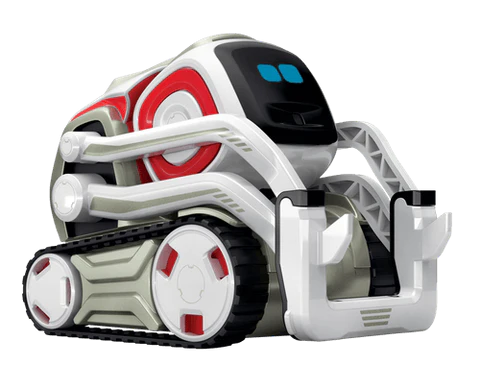
\includegraphics[height=3cm]{figures/cozmo.png}
            \caption{Cozmo}
        \end{subfigure}
        \begin{subfigure}{0.24\textwidth}
            \centering
            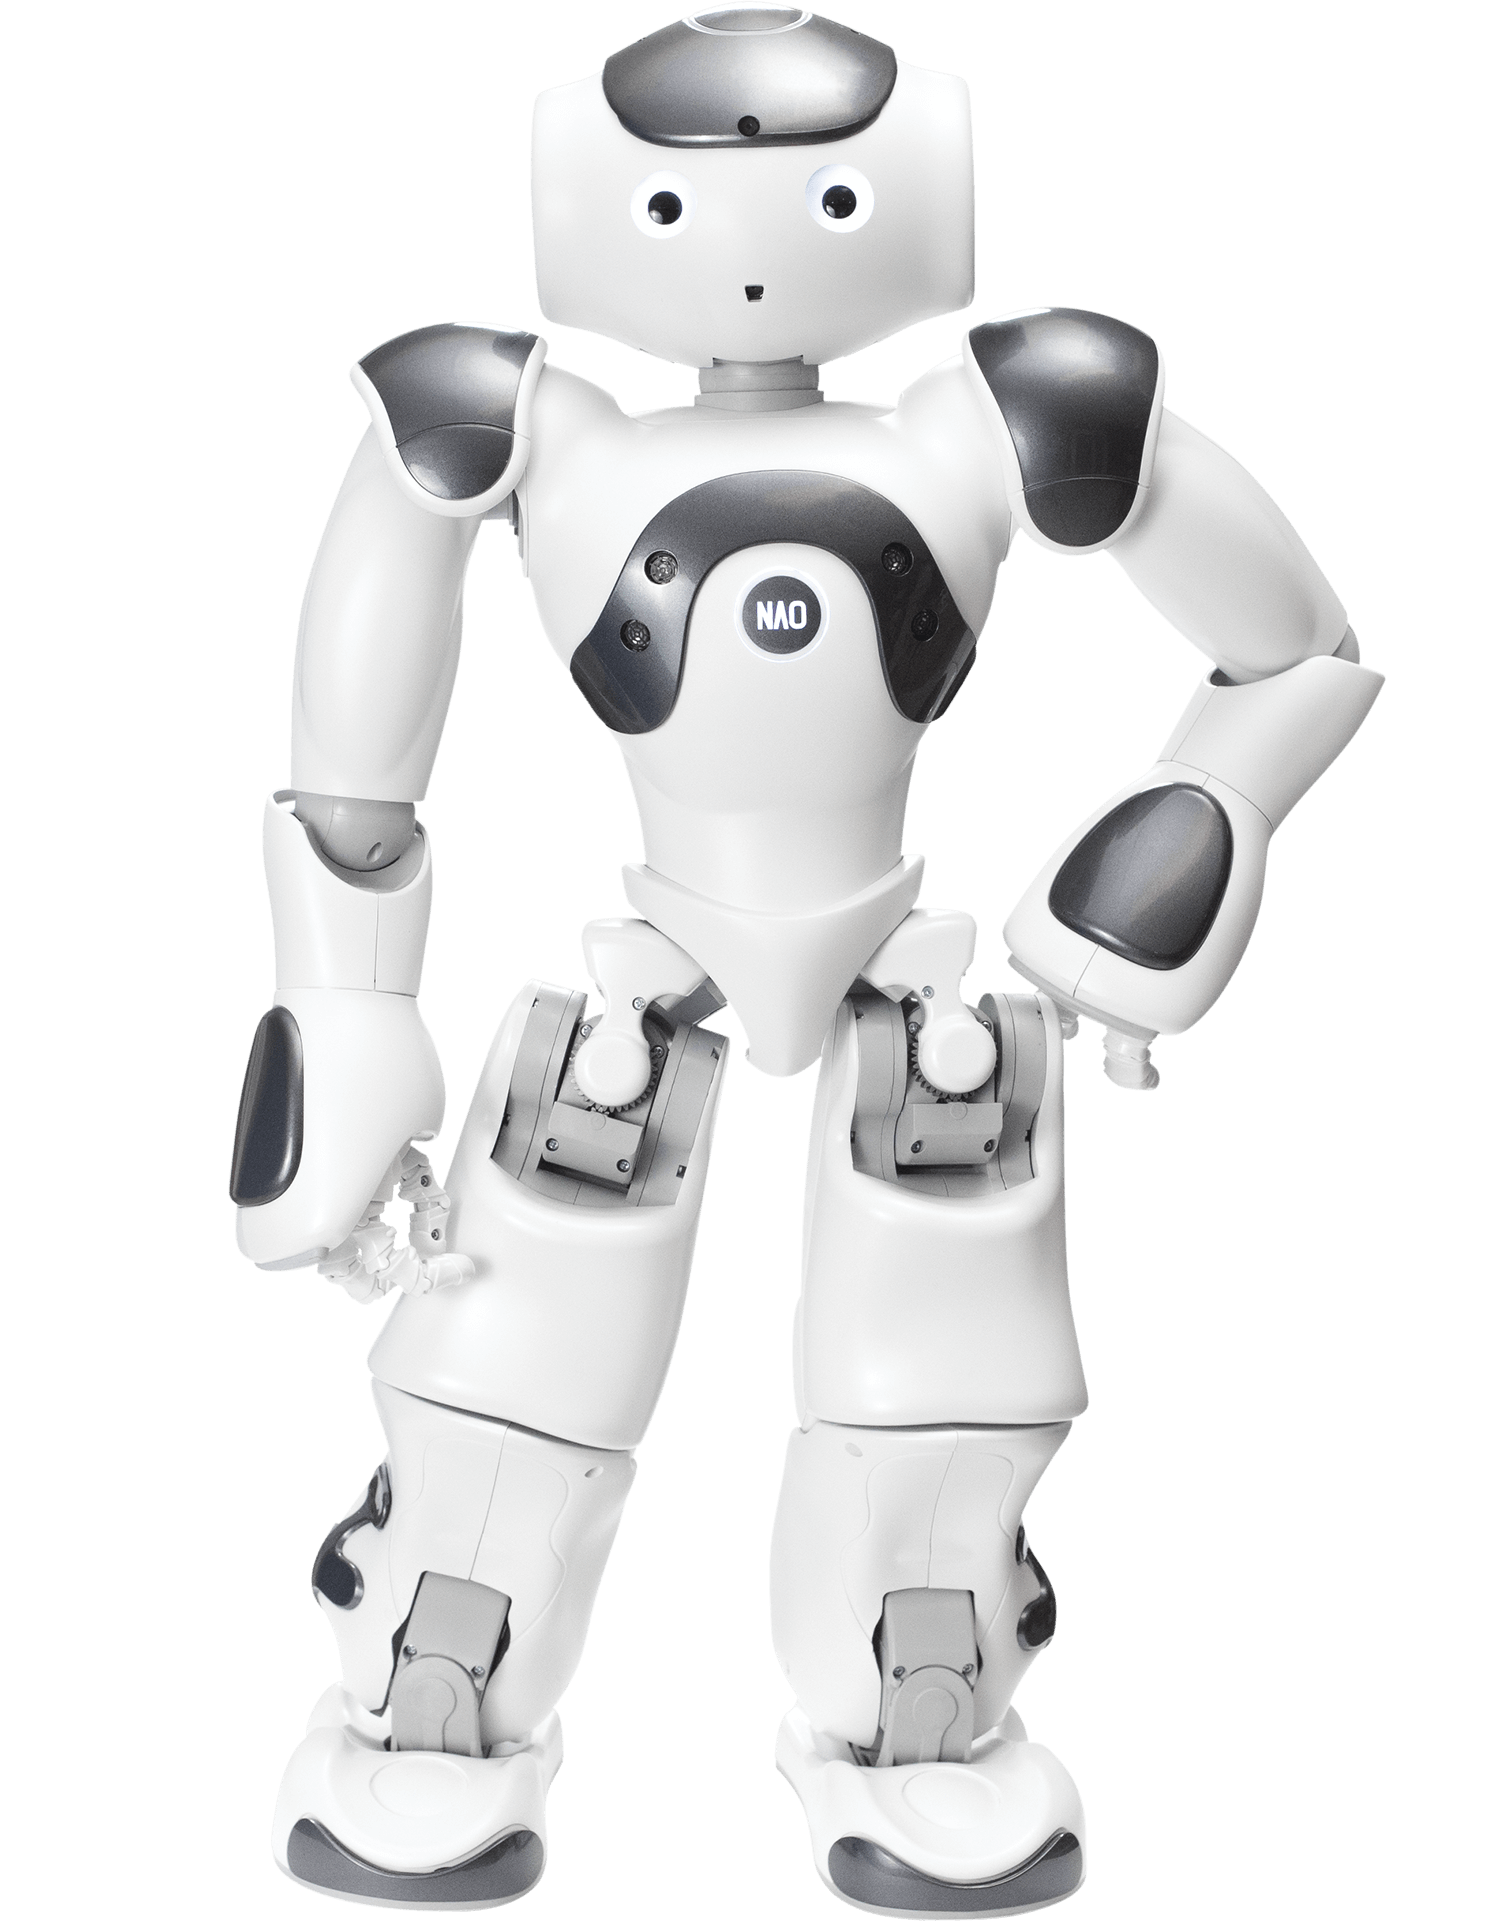
\includegraphics[height=3cm]{figures/nao.png}
            \caption{NAO}
        \end{subfigure}
        \begin{subfigure}{0.24\textwidth}
            \centering
            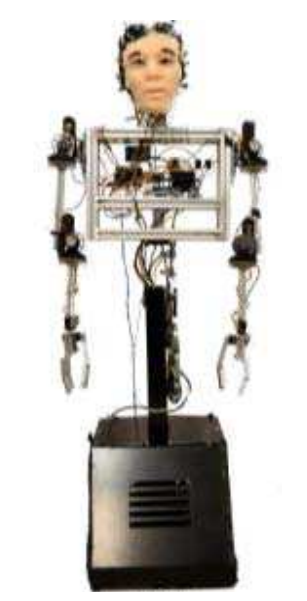
\includegraphics[height=3cm]{figures/brian.png}
            \caption{Brian}
        \end{subfigure}
        \begin{subfigure}{0.24\textwidth}
            \centering
            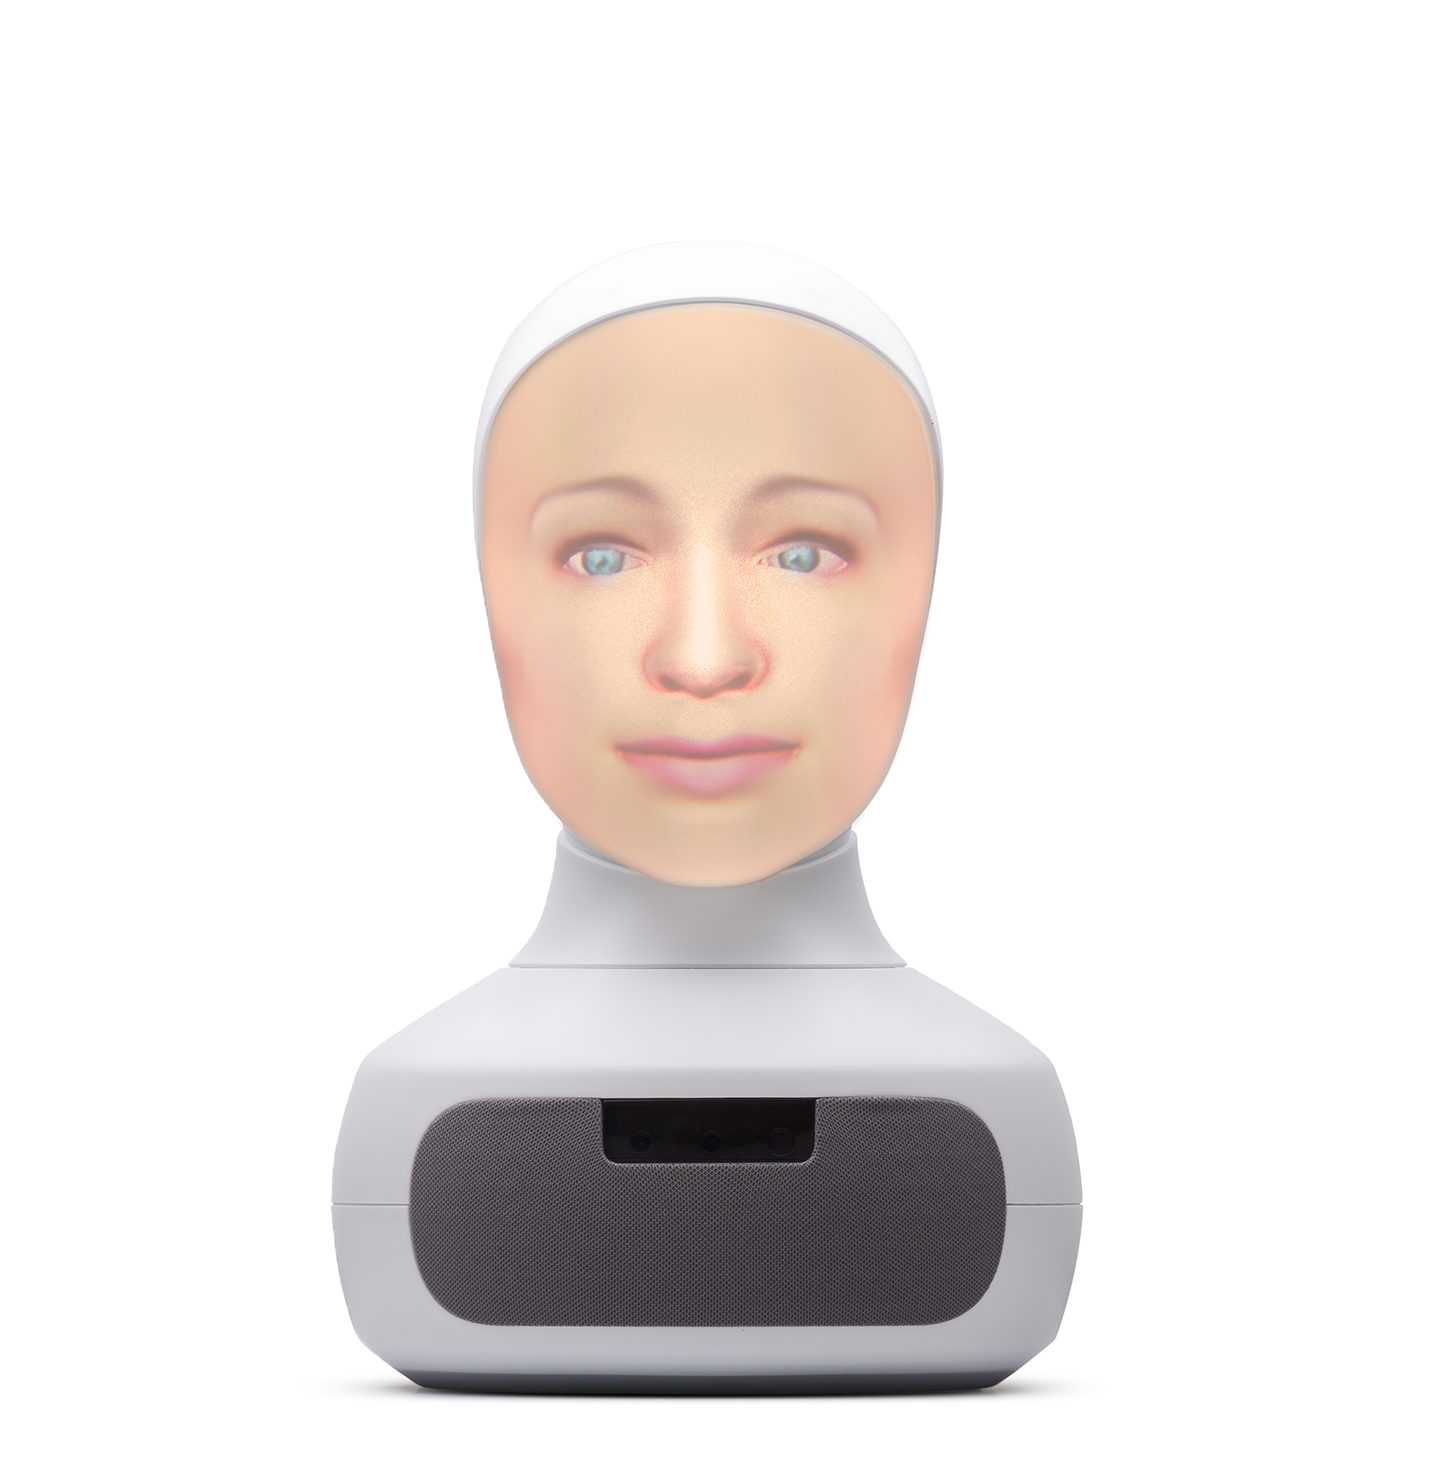
\includegraphics[height=3cm]{figures/furhat.png}
            \caption{Furhat}
        \end{subfigure}
    \end{subfigure}
    \caption{Figure of the appearance of the robots mentioned in the related works.}
    \label{fig:robots}
\end{figure}
\subsection{Personality in HRI}
The PERSONAGE language generator introduced earlier was used by \textcite{aly2013model} combined with the Behavior Expression Animation Toolkit (BEAT)~\cite{beat}. BEAT takes text as input and generates corresponding speech and gestures. These gestures are generated according to extensive human conversation studies and are able to transmit the implicit personality, motion characteristics, etc. contained in the language used. \textcite{aly2013model} evaluate this robot modelling on the same use case as \textcite{mairesse2007personage} (restaurant recommendations) using the humanoid robot NAO (see \Cref{fig:robots}). NAO mostly communicates through body movements and voice since it is incapable of expressing facial cues. \textcite{aly2013model} show that incorporating gestures increases the overall engagement and effectiveness of the robot. Furthermore, they found out that personality matching (in the Extraversion trait) with the user was favoured over the complementarity attraction principle suggesting that generally, in humans, a person with the opposite (complementary) characteristic should be preferred.

\textcite{andriella2020have} carried out a \gls{HHI} and \gls{HRI} study, evaluating the performance of a user in a memory game when helped by an agent capable of expressing personality (either human or robotic). The HHI study was conducted earlier also with the goal of recording the non-verbal cues of the subjects involved to later map them into the robot NAO. Similarly to~\cite{mairesse2007personage}, the authors only considered the extraversion trait and they also limited their scope to non-verbal interaction. Their findings include a better performance when the robot's extraversion trait matched that of the user and the opposite in the case of HHI.

\subsection{Emotion portrayal in HRI}
Convincing emotion portrayal has successfully been demonstrated with a variety of robots e.g. the educational toy robot Cozmo~\cite{cozmoEmotions}, NAO~\cite{desire} and the half-humanoid robot with a realistic human face Brain~\cite{brianEmotions}.

Cozmo (see \Cref{fig:robots}) was inspired by the robot Wall-E from the homonymous film with which shares its resemblance. Cozmo is designed to interact with the user through a series of simple noises, body and eye movements with which it is able to manifest some basic emotions as presets. The study from \textcite{cozmoEmotions} explores the role of a happy and sad response in the flow of interaction, finding that a sad expression has a natural reconsideration role while a happy expression would be understood as a continuation signal. In the case of sadness, the user would start questioning the past interaction in search of an explanation for the negative emotional change, and the user would interpret the happiness as a successful interaction. 

\textcite{desire} developed the DESIRE framework that aims at directly linking the user's voice to the emotional expression of NAO. This is achieved by understanding the Speed, Intensity, Regularity and Extent (SIRE) of the voice and mapping it to the robot's gestures. 

Brian (see \Cref{fig:robots}) is a robot developed by \textcite{brian} that has a human-like upper body and a face with artificial skin capable of facial expression. \textcite{brianEmotions} were able to incorporate 4 emotional responses to the interaction with the user in a task-completion context. The robot uses Markov chains and Q-learning to accurately transition from one emotion to the other with the goal of maximising the likelihood of the user completing the task. The tasks were multiple and varied from convincing the user to take a walk outside to going to the doctor for a scheduled appointment.

\subsection{At the intersection of (robot) personality and emotion}
There have also been works focusing on incorporating both personality and emotions into a robot. \textcite{moshkina2011tame} use the TAME framework~\cite{tame0, tame1} to incorporate (personality) Traits, Attitudes, Moods, Emotions into the robot NAO. They put these characteristics in descending order of time influence, starting with personality traits that do not change and last throughout life and ending with emotions that manifest in bursts and change very often even through a single conversation. These characteristics also have an ascending influence factor on speech and behaviour with emotions having the biggest influence and traits only slightly modifying the behaviour. The authors performed a successful preliminary exploratory
study with the robotic dog AIBO\footnote{\url{https://us.aibo.com/}} where they considered the personality traits of Extraversion and
Agreeableness and the emotions of Interest, Joy, Anger and Fear. They confirmed the correct reception of emotions and the recognition of the existence of a personality in the robot without, however, being able to distinguish between the different ones. A second study was conducted with the robot NAO where the personality was restricted to the Extraversion trait and the emotions to Fear and Joy. The results suggest an understanding of the personality and emotions expressed by the robot.

\textcite{han2012robotic} build and evaluate through a virtual head a framework that models the robot's emotional response based on the user's emotions, the robot's personality and current mood. In order to achieve this, they project the emotions in a 2D plane with pleasure-arousal as axes. The personality incorporation is limited to Openness, Extraversion, Agreeableness and Neuroticism (OEAN), therefore excluding the Conscientiousness trait. The personality is pre-programmed into the robot and affects the emotional response. The 4 traits are incorporated as continuous values and are parametrized into two weights corresponding to each one of the axes in the emotional plane. This system is then evaluated in a passive interaction scenario where the robot or rather, in this case, the virtual face manifested appropriate emotions in response to the user's talk.
\section{Summary}
\Cref{tab:related} shows a summary of all the related work regarding emotions and personality in the field of HRI with the last row being a description of this work.
Previous studies in \gls{HRI} clearly show some gaps in incorporating personality into robots, gaps that become even broader when restricting the scope to automated methods or language systems. In this chapter, we laid the foundations for the methods that will be used in the upcoming chapters to tackle this gap while also giving the reasons for doing it.

In particular, we will explore the text style transfer approach for personality generation and the incorporation of emotions through facial expressions in the robot Furhat~\cite{al2012furhat}, a social robot with human-like facial expressions and advanced conversational capabilities (see \Cref{fig:robots}). 
\begin{table}
    \centering
    \begin{adjustbox}{max width=\textwidth}
    \begin{tabular}{|c|c|c|c|c|c|c|c|}
        \hline
         & Robot & Emotions & Personality & Speech ability & Facial cues & Body cues & Scope \\
        \hline
        \hline
        \cite{andriella2020have} & NAO & \xmark & extraversion & \xmark & \xmark & \vmark & Task help\\
        \hline 
        \cite{cozmoEmotions} & Cozmo & sad, happy & \xmark & \xmark & \vmark & partial & Interaction flow\\
        \hline
        \cite{desire} & NAO & \vmark & \xmark & \xmark & \xmark & \vmark & -\\
        \hline 
        \cite{brianEmotions} & Brian & partial & \xmark & \vmark & \vmark & \vmark & Task completion\\
        \hline 
        \cite{mairesse2011controlling} & - & \xmark & \vmark & \vmark & \xmark & \xmark & Restaurant recommendation\\
        \hline 
        \cite{aly2013model} & NAO & \xmark & extraversion & \vmark & \xmark & \vmark & Restaurant recommendation\\
        \hline 
        \cite{moshkina2011tame} & AIBO & partial & OA (as weight) & \xmark & \xmark & \vmark & -\\
        \hline 
        \cite{moshkina2011tame} & NAO & joy, fear & extraversion (as weight) & \xmark & \xmark & \vmark & -\\
        \hline 
        \cite{han2012robotic} & Virtual Head & \vmark & OEAN (as weight) & \xmark & \vmark & \xmark & Listen and react\\
        \hline 
        \hline
        Ours & Furhat & \vmark & extraversion & \vmark & \vmark & \xmark & General\\
        \hline 
    \end{tabular}
    \end{adjustbox}
    \caption{Summary of the related work on emotions and personality in \gls{HRI} with the relevant features present.}
    \label{tab:related}
\end{table}
\cleardoublepage
\chapter{Methods}
\label{ch:methods}
The previous chapter outlined where this work sits with respect to \gls{HRI}. The use and the study of an interaction comprehending robots will be analysed in \Cref{ch:experiments} where we perform an in-depth evaluation using two user studies. In this chapter, we present all the datasets, methods and models that serve as technical side to power and automate the behaviour of such robots.

The first part of this chapter is concerned with the task of text style transfer of personality. We explored three different methods that take as input a text of general context and change its language (in terms of wording, etc.) depending on the personality that it should reflect. We focused for simplicity only on the extraversion trait. The technical work done in this part will be used to answer all of our research questions, and \hyperlink{rqs:1}{RQ1} in particular.

% with the goal of making a text convey a personality rather than another.
The second part of this chapter presents a way of linking personality to emotions in a meaningful way. As our personality manipulation is solely based on language, we explored multiple ways of extracting emotions from text. The methods we developed take some text as input and output the emotions that text triggers. This section of the work will be used to answer the part of \hyperlink{rqs:2}{RQ2} on emotional manifestation.

All the methods, models, data (later) collected and analysis done are stored in the following GitHub repository: \url{https://github.com/alessioGalatolo/Furhat-Personality-and-Emotions}.
% TODO: should be past tense except when you're following a standardized method
\section{Datasets}
The availability of datasets containing utterances classified with personality labels is very restricted. Furthermore, the few datasets that do are often limited in terms of topic and context of the utterances and in terms of size. Another limitation is the use of different personality frameworks (Big 5 and \gls{MBTI}, as presented in \Cref{sec:personality}) and the unavailability of a continuous scale for the traits that are almost always presented as binary. This is expected in the case of the \gls{MBTI} framework but is also very frequent even in the case of the Big 5. Reasons for preferring a continuous scale are intrinsic in the definition of personality as each trait can present itself in various degrees (e.g. a person that is 51\% extrovert may behave very differently from one that is 99\% extrovert). Also, personality is considered an invariant in the life of a person and using a binary scale to describe a person may bring different results at different times due to measuring errors (e.g. a 51\% extrovert person, considered extrovert at some point, may later be a 49\% person which would fall under the introvert grouping). However, categorical labelling for the personality is very suitable for the text style transfer approach described in \Cref{sec:styletransfer} where in almost all of the works the style is considered categorical.

The datasets that we were able to collect are shown in \Cref{tab:datasets}. The Essays dataset~\cite{pennebaker1999linguistic} is a dataset comprehending 2467 stream-of-consciousness essays written by psychology students that were classified into binary Big-5 personality traits through a self-report questionnaire. The MBTI dataset\footnote{\url{https://www.kaggle.com/datasets/datasnaek/mbti-type}} is a collection of posts from the \href{https://www.personalitycafe.com/}{Personality Cafe Forum} where users have completed a 102-items personality test\footnote{\url{https://similarminds.com/embj.html}}, the labels follow the \gls{MBTI} framework. The personality-detection (Friends dataset)~\cite{jiang2020automatic} is a collection of 710 utterances extracted from the American sitcom `Friends', here \textcite{jiang2020automatic} labelled through crowd-sourcing the personality of each utterance. The PERSONAGE dataset~\cite{mairesse2007personage, mairesse2011controlling} is a collection of 580 utterances about restaurant recommendations and comparisons. 260 of them are only rated on the extraversion trait and were assessed by three expert judges. The reaming sentences are rated on the whole Big-5 framework by 24 subjects. The rating ranges from 1 to 7. We used the MBTI and Essays datasets for training our models, the PERSONAGE and Friends ones for evaluation. PERSONAGE was also used for training in some cases.

Finally, another dataset that was used in this thesis is the NRC Lexicon dataset~\cite{mohammad2013crowdsourcing}, this crowd-sourced dataset contains a list of 14182 words and each word has been rated on 8 emotional (binary) scales: Positive, Negative, Anger, Anticipation, Disgust, Fear, Joy, Sadness, Surprise and Trust. This dataset was used to create an emotion classification model, such that the stylised text output by the language models can be automatically assessed for emotional labels, which can be fed to the robot platform for the automatic generation of appropriate emotional expression.

Another dataset that was used that is, however, not concerned with neither emotions nor personality is the Yelp dataset\footnote{\url{https://www.yelp.com/dataset}}. This dataset was used to confirm the correct implementation of our first text style transfer method. The dataset contains a set of reviews from Yelp that are labelled as either positive (e.g. ``This place was fantastic") or negative (e.g. ``This place was horrible"). They sever for the task of transferring the sentiment i.e. from a negative sentence to a positive one and vice-versa.
% Other datasets that were used are the Twitter COVID dataset~\cite{banda2021large} and the Twitter Sentiment140 dataset~\cite{go2009twitter}. The former comprehends 133933 tweets on the topic of COVID-19 while the latter 1600000 tweets without a specific topic. Both were treated as unlabelled dataset and the personality label is later inferred from other methods.
\begin{table}
    \centering
    \begin{adjustbox}{max width=\textwidth}
        \begin{tabular}{|p{0.19\textwidth}|p{0.19\textwidth}|p{0.19\textwidth}|p{0.19\textwidth}|p{0.19\textwidth}|}
        \hline
        Name & Size & Origin & Labels & Labelling method \\
        \hline
        \hline
        Essays & 2467 essays & Students' stream-of-consciousness essays & Binary Big-5 & Self-report questionnaire\\
        \hline
        MBTI & 8600 users' posts & PersonalityCafe forum & \gls{MBTI} & 102 items personality test\\
        \hline
        Friends & 710 utterances & Friends & Binary Big-5 & Crowd-source\\
        \hline
        PERSONAGE & 580 utterances & PERSONAGE generator & 1 to 7 Big-5 for 320, only extraversion for 260 & \gls{TIPI}~\cite{gosling2003very}\\
        \hline
        NRC Lexicon & 14182 words & - & Binary,  6 emotions + 2 sentiments & Crowd-source\\
        \hline
        Yelp & 638943 reviews & Yelp & Positive/negative & -\\
        \hline
        % Twitter COVID & 133933 English tweets & Twitter & - & -\\
        % \hline
        % Twitter Sentiment140 & 1600000 English tweets & Twitter & - & -\\
        % \hline
        \end{tabular}
    \end{adjustbox}
    \caption{List of the datasets collected and used in this thesis and their attributes.}
    \label{tab:datasets}
\end{table}
\section{Text style transfer models}
% In order to assess the best model to generate language that is influenced by personality, we have explored multiple models that will be described in the following sections. 
This section overviews the various models used for the text style transfer of personality. Similarly to many previous works we will limit the personality manipulation to the extraversion trait. Also, following the concerns outlined in \Cref{sec:llm} about \gls{LLM}, we decided to try 3 different language models varying in their size (number of parameters). We will present, in this order, a model that needs to be trained from scratch with a low number of parameters ($\sim$30 million, \Cref{sec:gan_based}), a pretrained model that needs to be fine-tuned for our task with a medium number of parameters ($\sim$1.5 billion, \Cref{sec:strap}), and a \gls{LLM} with a high number of parameters ($\sim$175 billion, \Cref{sec:gpt3}).

These models will be used in our pipeline (see \Cref{fig:system_flow}) as input for the speech of the robot. The computational time of these models is especially relevant given this use case.
\section{GANs with language models}
\label{sec:gan_based}
The first model that was used is an implementation of the model presented in~\cite{yang2018unsupervised}. Here, the authors borrow concepts from \gls{CV} and adopt a \gls{GAN} approach to the text style transfer task. \Glspl{GAN} are generally made up of two parts: a generator $G$ and a discriminator $D$ that are trained together. The generator's aim is to generate samples e.g. images in \gls{CV} or utterances in our case, while the discriminator is used to check whether the samples are realistic and respect the wanted properties e.g. believable images in \gls{CV} or utterances with the right style in our case. \textcite{yang2018unsupervised} combine an attentional Auto-Encoder for the generation part with a classifier for the discrimination part. In the first stage of the training, the auto-encoder's goal is to output the same sentence it is given as input, while the classifier is trained to recognise the style (or the personality in our case) of that same sentence (the goal of the classifier won't change throughout the training). 

Let $x$ be an input sequence and $y$ its original style, then, the generator's goal in this phase is to output a sentence as close as possible to the input one (auto-encoding objective):
\begin{equation*}
loss_G^{pre} = l_G^{ae} = SCE(G(x), x).
\end{equation*}
Where $SCE$ is softmax cross-entropy. The discriminator's objective is to correctly classify the sentence:
\begin{equation*}
loss_D = BCE(D(x), y).
\end{equation*} 
Where $BCE$ is binary cross-entropy. This stage is followed by a second one where the generator is trained to output sentences with a different style than the input e.g. $style(G(x)) \neq y$. More specifically, in the case of text style transfer where we want to go from one style to the other, we would have only 2 styles encoded as 0 and 1. In this case the objective is: $style(G(x)) = |1-y|$. This is done by using the classifier as a discriminator or as the $style$ function. The generator's loss is now a weighted sum of the previous one and the loss coming from the class of the output sequence:
\begin{equation*}
loss_G = l_G^{ae} + \lambda_g BCE(D(G(x)), |1 - y|).
\end{equation*}

\subsection{Implementation details}
The original authors implemented this method using the open-source framework TensorFlow (version 1.15)\footnote{\url{https://github.com/tensorflow/tensorflow/tree/r1.15}} and the Texar toolkit\footnote{\url{https://github.com/asyml/texar}}. Texar is an open-source toolkit for \gls{NLP} and language generation. It provides implementations of popular language models as well as utilities for implementing new ones. Texar is compatible with both TensorFlow (up to version 1.15) and PyTorch\footnote{\url{https://github.com/pytorch/pytorch}} frameworks.

The original method from the authors needed an adaptation to our task due to the different nature of the problem. This process, however, turned out to generate multiple problems and errors (also caused by the use of an old version of TensorFlow - the current one is 2.8). For this reason, we re-implemented the model using the PyTorch framework and the relative Texar version. We did not change the architecture of the method when re-implementing it.
\subsection{Training}
\label{sec:gan_training}
Before training for the task we were posed, we reproduced the work of \textcite{yang2018unsupervised} on the Yelp dataset in order to assess the correct implementation of the original method. The version of the Yelp dataset used by the authors consists of 638,943 reviews labelled on sentiment i.e. positive or negative reviews. The task consists of transferring positive reviews into negative ones and vice-versa.

We then tested this model on our problem by training on two different datasets. The first dataset was extracted from the Essays one. Here, each essay was split into single sentences following punctuation. Each sentence was labelled with the original extraversion binary trait of the essay's author. The new dataset is made up of 91359 sentences where 45295 of them are from an extrovert person ($\sim$50\%) and the rest is from introverts. The second dataset is the MBTI one. Similarly to the Essays dataset, we split each post into single sentences resulting in a total of 788897 utterances. However, only 186526 of these were extroverted ($\sim$24\%). Believing that this unbalance in the classes could result in a biased classifier (of personality) that does not generalise well enough, we used an undersampling technique where the classifier was trained with an equal amount of text from introverts and extroverts (186526 for each). For all the datasets, the maximum length of a sentence was 20 words, this constraint was given by the original authors and was motivated by better performances on shorter sentences.

The reason for using these two datasets among all of those presented earlier mainly lies in their size. In fact, contrary to these two datasets that can be expanded into single sentences, both the Friends and the PERSONAGE datasets are already composed of single utterances. Further, since the proposed method does not contain any previous knowledge of natural language (i.e. has not been pretrained in any way), it requires as much data as possible. Nevertheless, we opted to use both PERSONAGE and Friends datasets for the evaluation of this method.
\subsection{Results on Yelp dataset}
As introduced in \Cref{sec:gan_training} we did 3 experiments with this model, the first aimed at assessing the correct reproduction of the model, while the others aimed at testing its capabilities in our task. For each experiment, we report the accuracy graph, training time and qualitative evaluation of the transferred text. For the experiments in our task, we also report the quantitative performance of the classifier. All of these experiments have been done on a single NVIDIA GeForce RTX 2080 Ti GPU with 10GB of dedicated memory and on a machine with 10GB of RAM (allocated to the training). To keep track of the training time, accuracy, resource consumption, etc. we used the \gls{ML} platform Weights \& Biases\footnote{\url{https://wandb.ai/site}}.

To first assess the correct implementation of this model, we tested it on the same settings as its authors (\textcite{yang2018unsupervised}). The model was trained for 12 epochs where the first 10 were of pretraining. 
\begin{figure}
    \centering
    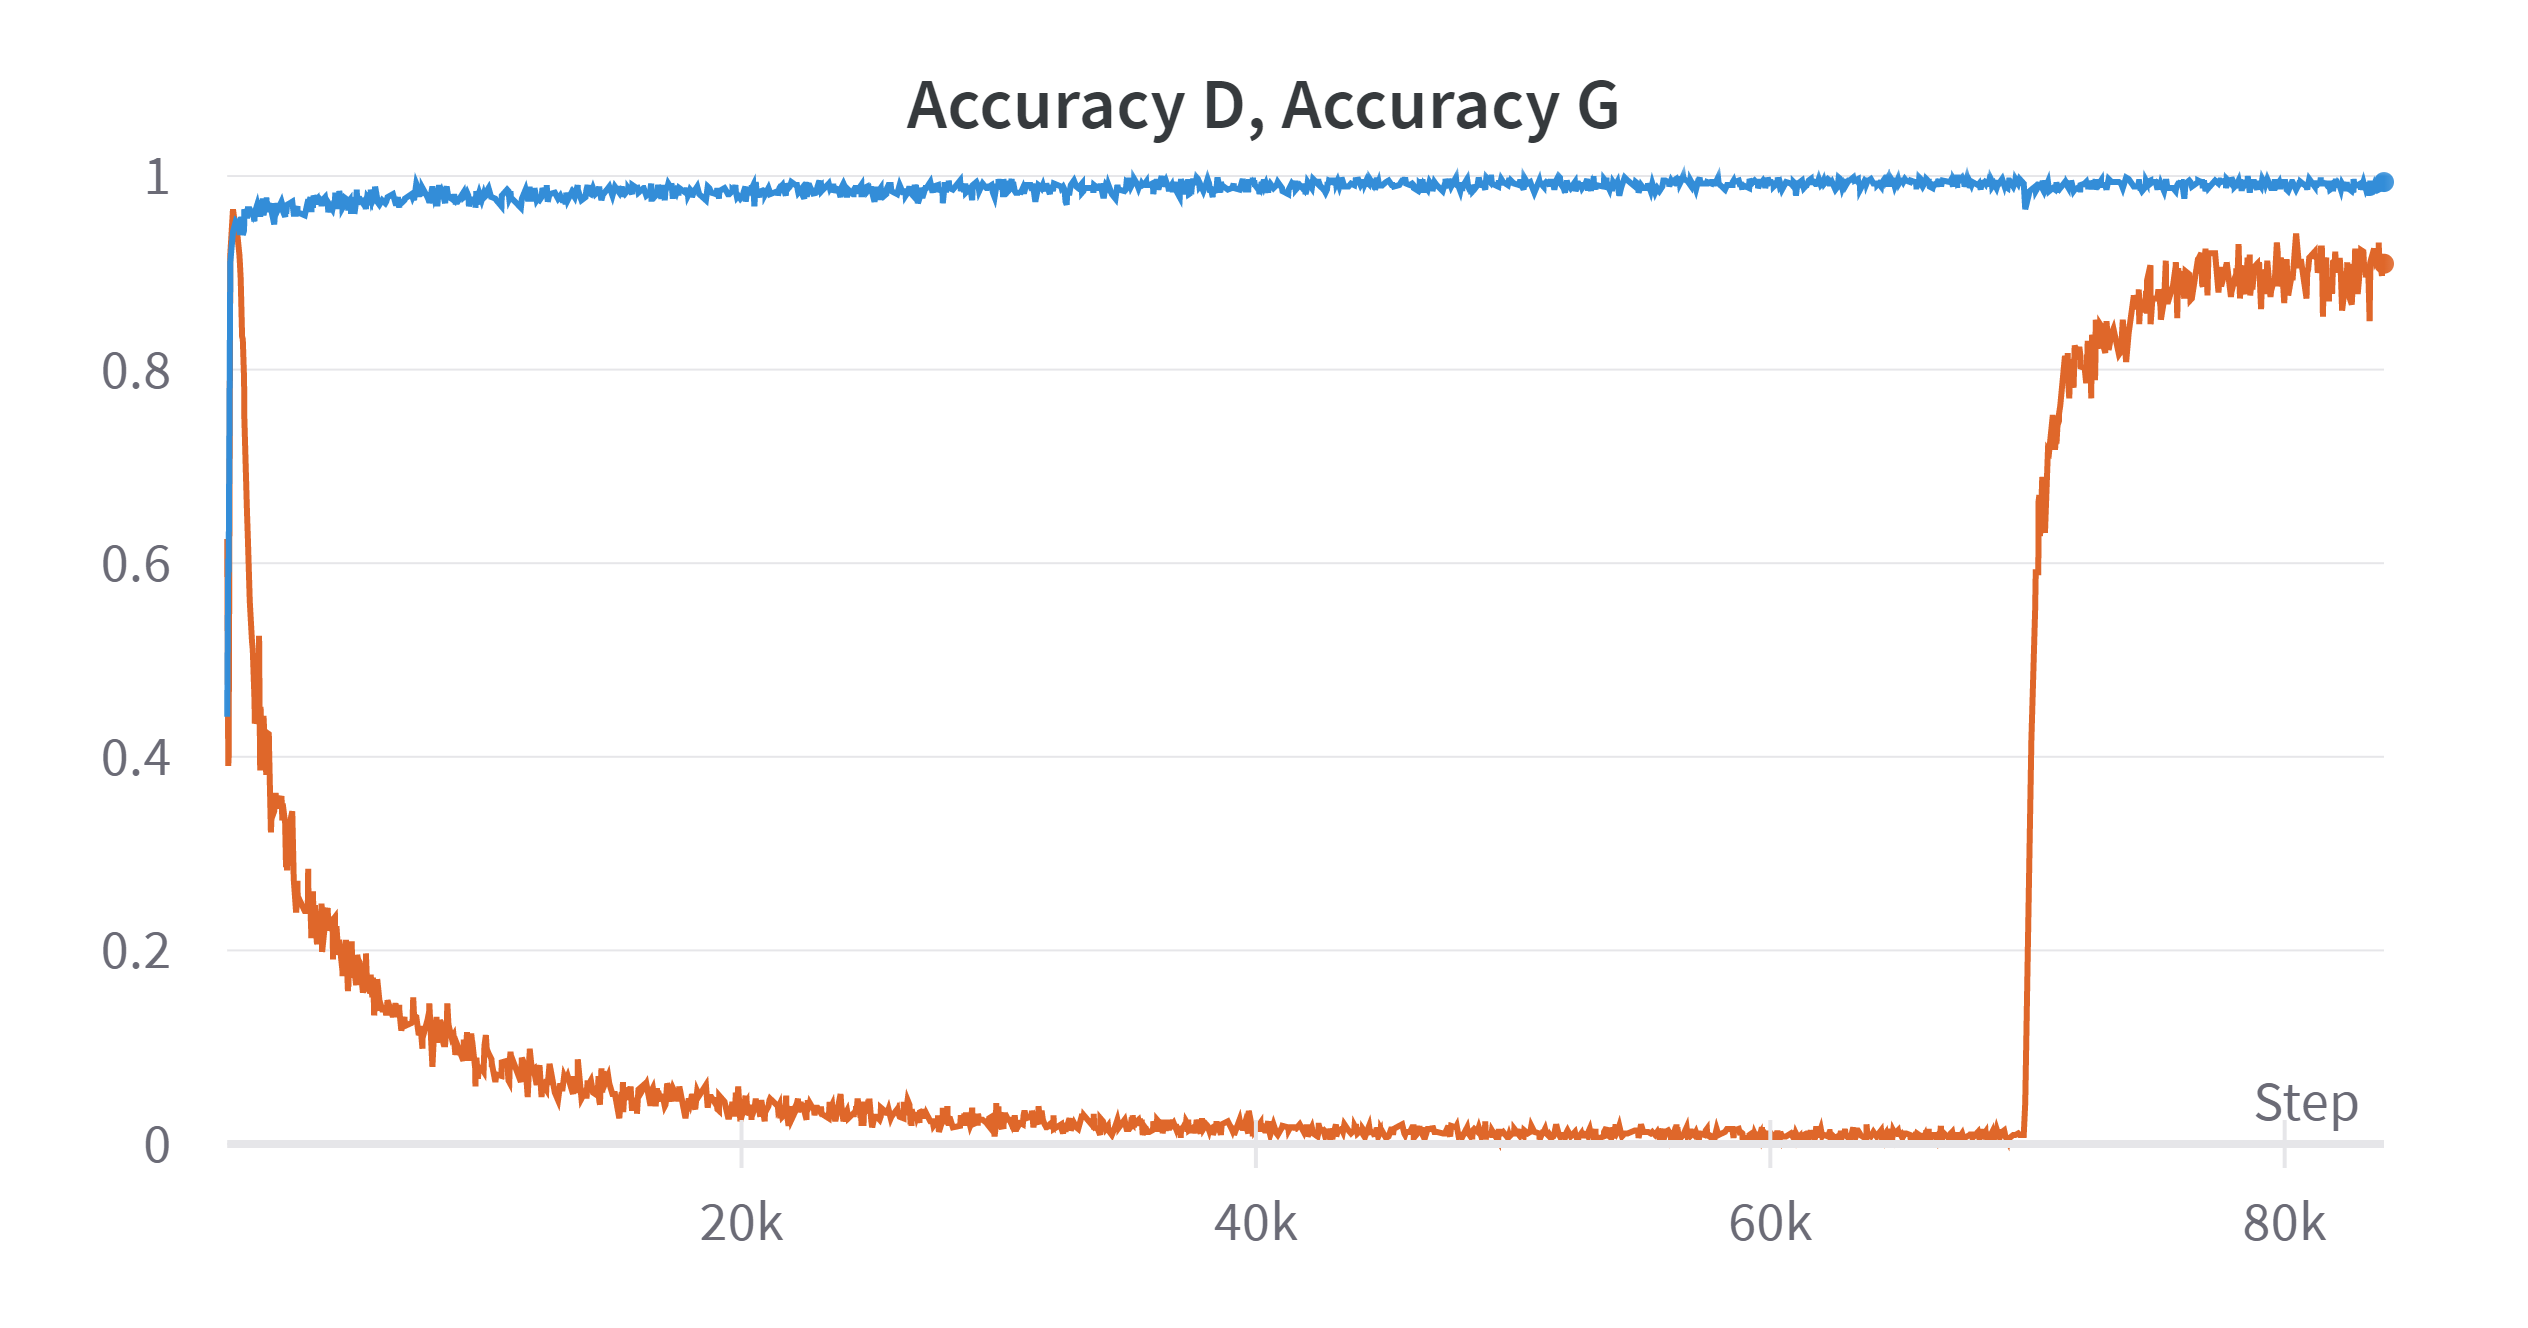
\includegraphics[width=\textwidth]{figures/yelp training.png}
    \caption{Training accuracy on the Yelp dataset. The classifier (D) accuracy is in blue quickly approaching 1, while the generator's (G) is in orange, quickly approaching 0.}
    \label{fig:yelp_training}
\end{figure}
\Cref{fig:yelp_training} shows the progression of the training accuracy for the generator (G) and the classifier (D). It is possible to notice how the accuracy for the classifier constantly increases, approaching 1, while the generator approaches 0. This is however expected, as throughout the training we compute the accuracy of the generator as its ability to transfer the style of the input sequence but the generator is first trained as an auto-encoder making it output the same exact sequence. Therefore, as the classifier gets better at recognising the style and the generator gets better at outputting the same sequence, its accuracy must decrease. Once, however, the pretraining ends and we start training with the goal of transferring the style, the accuracy of the generator naturally spikes, approaching 90\%. 

\begin{table}
    \centering
    \begin{adjustbox}{max width=\textwidth}
        \begin{tabular}{|p{0.13\textwidth}|p{0.29\textwidth}|p{0.29\textwidth}|p{0.29\textwidth}|}
        \hline
        Sentiment & Input & Our Output & Original Output \\
        \hline
        \hline
        Positive & Go to place for client visits with gorgeous views. & Go to place for client visits with \textbf{mushy} views. & Go to place for client visits with \textbf{lacking} views.\\
        \hline
        Positive & There was lots of people but they still managed to provide great service. & There was lots of people but they still managed to provide \textbf{tasteless} service. & There was lots of people but they still managed to provide \textbf{careless} service.\\
        \hline
        Negative & Needless to say, we skipped desert. & Needless to say, we \textbf{delicious} desert. & Gentle to say, we \textbf{edgy} desert. \\
        \hline
        Negative & The first time i was missing an entire sandwich and a side of fries. & The first time i was \textbf{tanya} an entire sandwich and a side of fries. & The first time i was \textbf{beautifully} an entire sandwich and a side of fries.\\
        \hline
        \end{tabular}
    \end{adjustbox}
    \caption{Some of our test results on the Yelp dataset and a comparison with the original implementation. Changes in the output are marked in \textbf{bold.}}
    \label{tab:yelp_results}
\end{table}
The training lasted 8h20m and the final accuracies are 99.22\% for the classifier and 89.92\% for the generator. The inference using this method does not require high resources (i.e. no GPU is needed) and its generation is almost instantaneous. \Cref{tab:yelp_results} also reports some results after the training for a qualitative evaluation. We can see the method is able to identify the parts of a sentence that make it `positive' rather than `negative' and substitutes them with attributes from the opposite style. Sometimes the results appear unnatural due to verbs being substituted with substantives and similar.
\subsection{Results on Personality datasets}
After confirming the correct reproduction of the original method we proceeded to train it on the Essays and MBTI datasets. The progression of the training accuracy is shown in \Cref{fig:mbti_essays_results} for the MBTI and Essays dataset.
\begin{figure}[ht]
    \centering
    \begin{subfigure}{\textwidth}
        \centering
        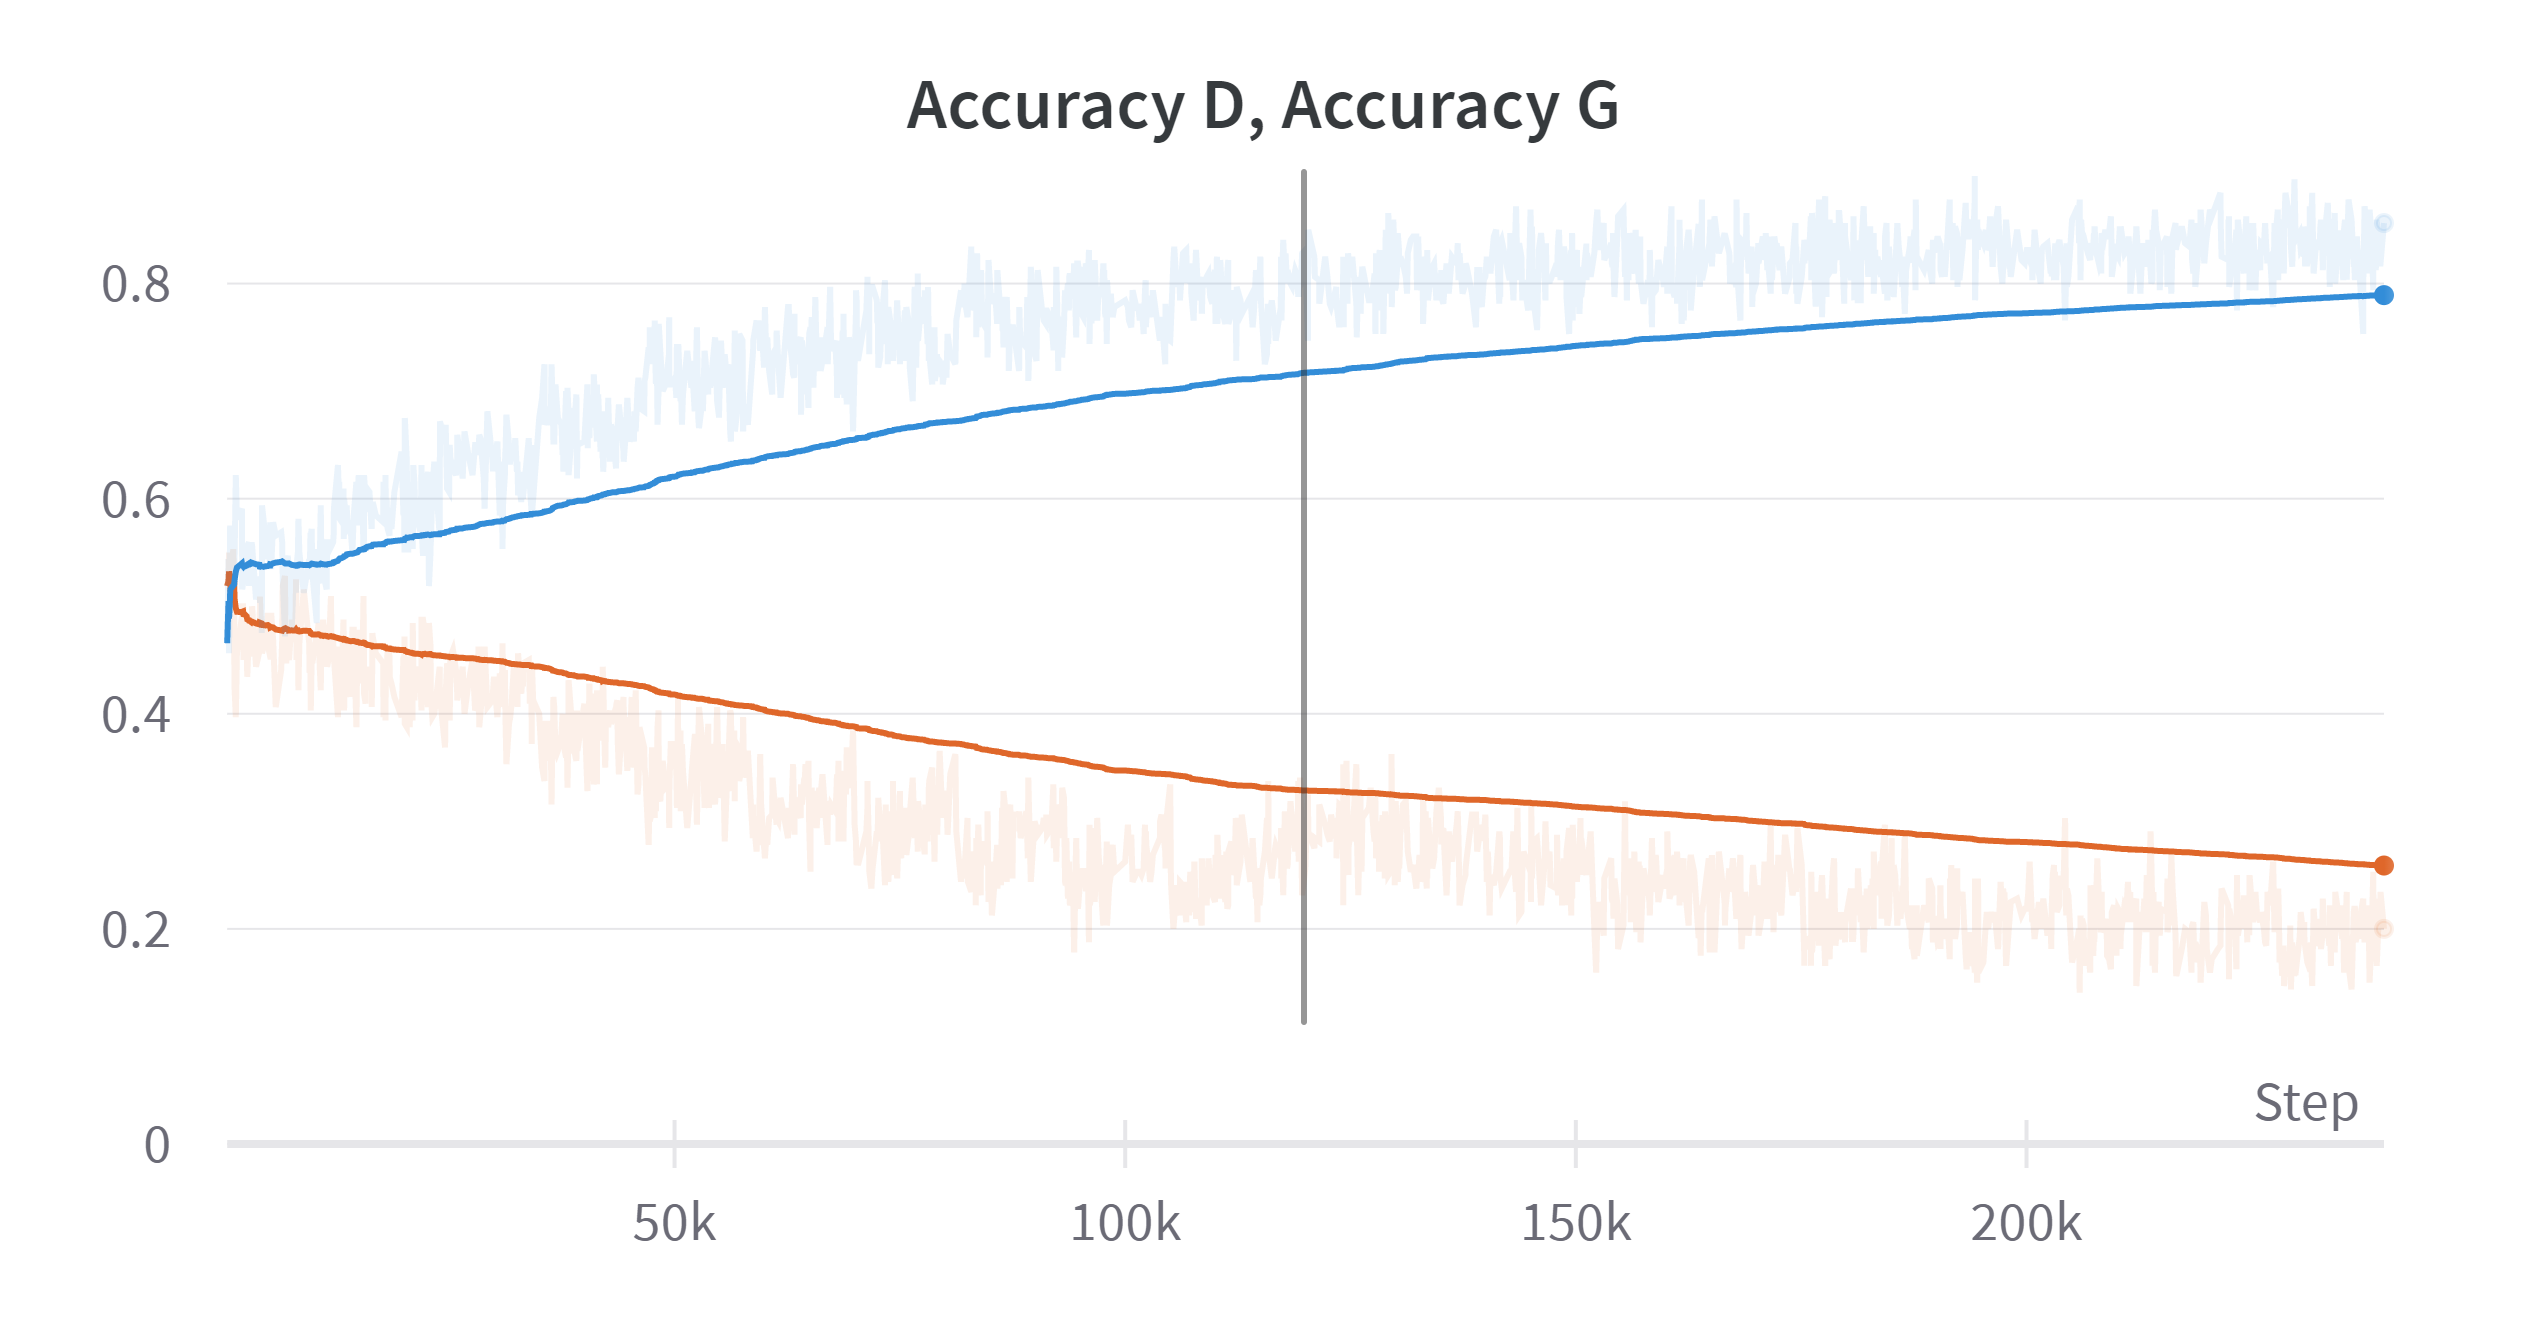
\includegraphics[width=0.7\textwidth]{figures/mbti training smoothed.png}
        \caption{MBTI}
    \end{subfigure}
    \begin{subfigure}{\textwidth}
        \centering
        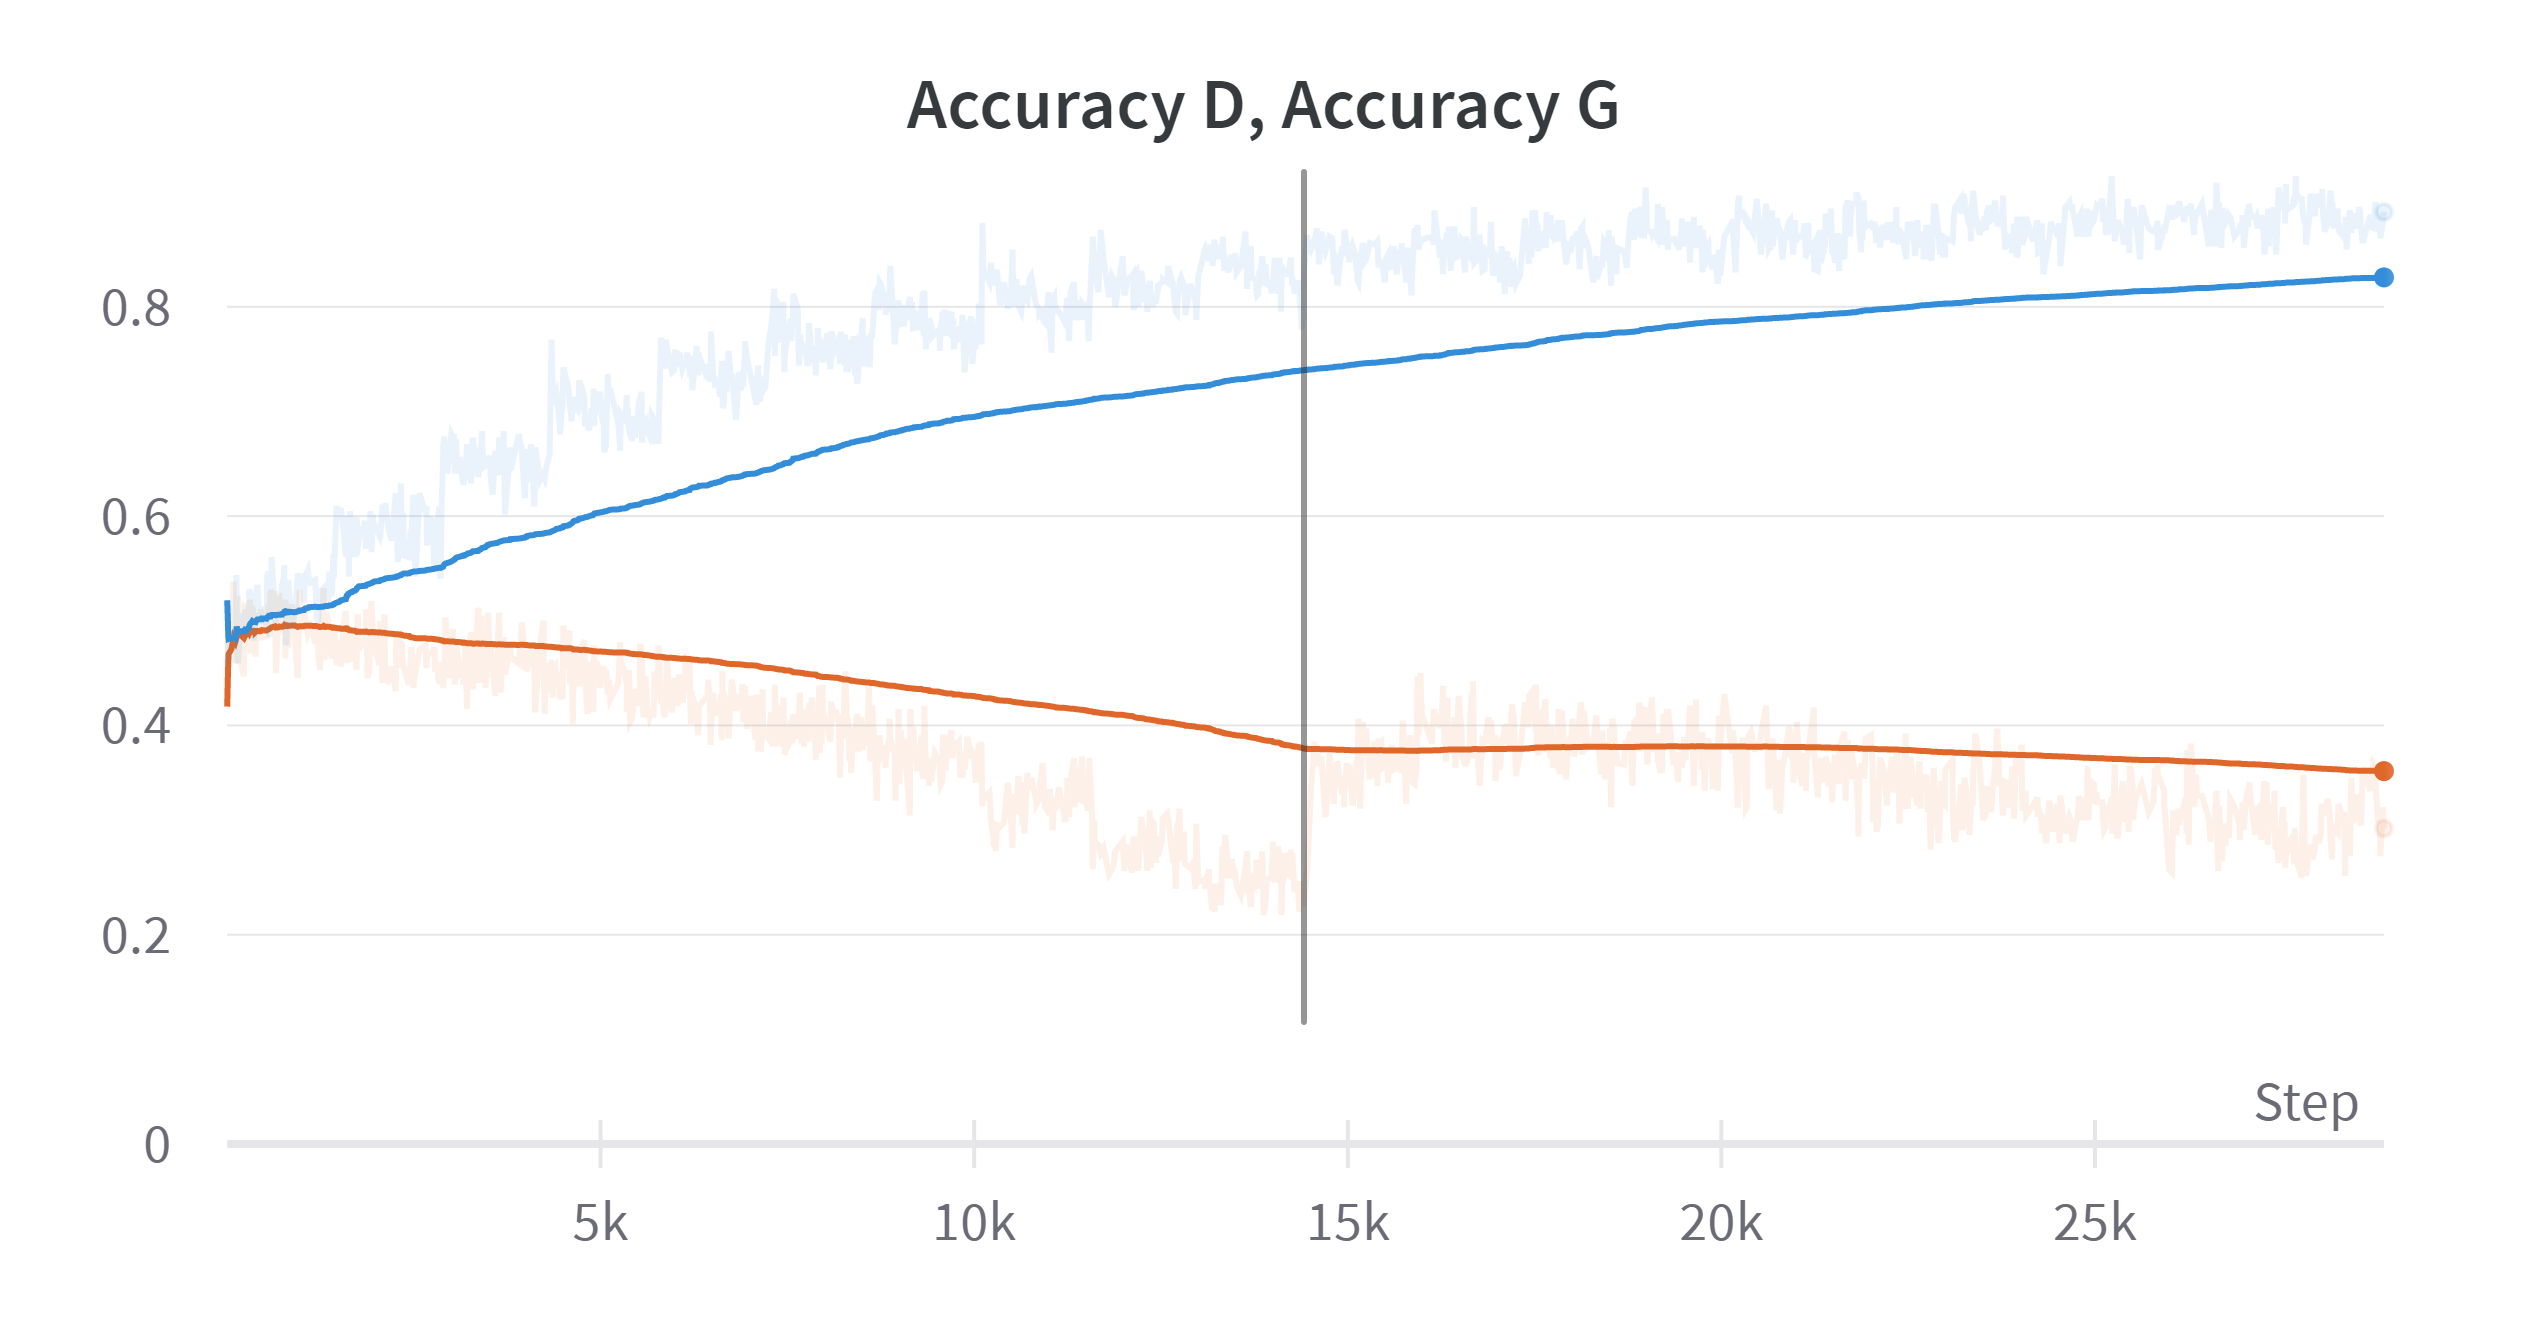
\includegraphics[width=0.7\textwidth]{figures/essays training smoothed.png}
        \caption{Essays}
    \end{subfigure}
    \caption{Training accuracy on the MBTI (above) and Essays (below) dataset. The training curve is in the background while we highlight its smoothed version for better reading. The line in the middle of the graph splits is the boundary of the pretraining. The classifier (D) accuracy is in blue quickly approaching 1, while the generator's (G) is in orange, quickly approaching 0.}
    \label{fig:mbti_essays_results}
\end{figure}
It is possible to see how the graphs have a very similar progression. Both the classifier and the generator's accuracy are slower in increasing and decreasing respectively if compared to the Yelp dataset. The graph also shows how the auto-encoding objective is mostly fulfilled for the pretraining. However, when trained with the style transfer objective the accuracy starts plummeting after a small, initial, increase (more evident in the Essays' case). From the graph alone, we expect the method not to be very successful in our task as the utterances retain the same style (according to the discriminator) more than half the time even after being processed through the generator. 

For both datasets, we used the same number of pretraining epochs of the Yelp dataset (10) but we increased the total number of epochs to 20. The training time is 4h, and $\sim$59h for the Essays and MBTI respectively. Similarly to the Yelp case, the inference is not resource-intensive and takes a negligible amount of time.
\subsubsection{Generator performance}
The final generator accuracy is $\sim$30\% (spiking at $\sim$46\%) for Essays and 17.50\% (spiking at $\sim$35\%) for MBTI. We were able to test the performance of the generation both at the end and at intermediate times by saving many checkpoints of the model throughout the training. As the results did not vary much after the pretraining phase, we only report, in \Cref{tab:mbti_essays_results}, the final generations. We used the PERSONAGE and Friends dataset as the source of the sentences. It is possible to see how the MBTI one rarely changes any words in the sentence, with two sentences that don't change at all after the generation. The times when it does actually change some words, these appear nonsensical\footnote{Of course, the model does not actually `make up' words, the wording just reflects the dataset it was trained on. Both the MBTI and Essays dataset contain `made up' words as one is in the informal context of a forum and the other follows the stream-of-consciousness narrative method.} or out of context. On the other hand, even though the Essays one changes wording quite more often it also tends to put random words out of context with some of them being, again, made up.
\begin{table}
    \centering
    \begin{adjustbox}{max width=\textwidth}
        \begin{tabular}{|p{0.15\textwidth}|p{0.40\textwidth}|p{0.40\textwidth}|p{0.40\textwidth}|}
        \hline
        Transfer direction & Input & MBTI output & Essays output \\
        \hline
        \hline
        Ext $\rightarrow$ int & Japonica is a Japanese, Sushi restaurant, with excellent food quality and decent decor. Dojo, which is a Japanese, Vegetarian restaurant, with decent food quality, has mediocre decor. & \textbf{Mormonism} is a Japanese, Sushi restaurant, with excellent food quality and decent decor. \textbf{Gov}, which is a Japanese, Vegetarian restaurant, with decent food quality, has mediocre decor. & \textbf{Marriage} is a Japanese, \textbf{iw} restaurant, with excellent food quality and decent \textbf{obligations}. \textbf{Deadlines}, which is a Japanese, \textbf{iw} restaurant, with decent food quality, has \textbf{quicker icq}.\\
        \hline
        Int $\rightarrow$ ext & I don't know. Ac-ac-actually, I would ap-ap-approve Vinnie's Pizza. It's a pizza place. Even if it's bloody cheap, I mean, it features like, really bad ambience. It provides rude staff. & I don't know. \textbf{Gettingbackontrack} ac-actually, I would \textbf{relied harboring approve EASY's Pizza}. It's a pizza place. Even if it's bloody cheap, I mean, it features like, really bad \textbf{enough}. It provides rude staff. & I don't know. \textbf{Whitis edge} actually, I would \textbf{roaming stumbled emails Erica's} Pizza. It's a pizza place. Even if it's \textbf{al} cheap, I mean, it \textbf{calle} like, really bad \textbf{miscommunication}. It provides rude staff.\\
        \hline
        Ext $\rightarrow$ int & I know, I know, I'm such an idiot. I guess I should have caught on when she started going to the dentist four and five times a week. I mean, how clean can teeth get? & I know, I know, I'm such an idiot. I guess I should have caught on when she started going to the dentist four and five times a week. I mean, how clean can teeth get? & I know, I know, I'm such an idiot. I guess I should have caught on when she started going to the \textbf{dwarfs} four and five times a week. I mean, how clean can teeth get?\\
        \hline
        Int $\rightarrow$ ext & Alright Ross, look. You're feeling a lot of pain right now. You're angry.  You're hurting.  Can I tell you what the answer is? & Alright Ross, look. You're feeling a lot of pain right now. You're angry.  You're hurting.  Can I tell you what the answer is? & Alright \textbf{black}, look. You're feeling a lot of pain right now. You're angry.  You're hurting.  Can I tell you what the answer is? \textbf{About stability Born Vaughn issuses Sampras issuses substances issuses wages}\\
        \hline
        \end{tabular}
    \end{adjustbox}
    \caption{GAN-based model generations when trained on the Essays and MBTI dataset. First two sentences are from PERSONAGE dataset, second two from Friends dataset. Changes in the output are marked in \textbf{bold.}}
    \label{tab:mbti_essays_results}
\end{table}
\subsubsection{Classifier performance}
\label{sec:gan_classifier}
Contrary to previous works, we decided to use the whole dataset (either MBTI or Essays) to train our model without leaving any samples for the evaluation of the personality classifier. Evaluating the model on the same dataset would probably show better performance as the samples would be at least similar to those in the training set. However, this would not reflect real-world performance. As our final goal is to apply the outlined methods to a User Study, we expect the relative dialogues to be free from any constraints and to not be similar to any particular dataset. For this reason, the evaluation of the classifier has been done on the Friends and PERSONAGE datasets plus the MBTI dataset if trained on the Essays and vice-versa and it is shown in \Cref{tab:mbti_essays_classifier}. Further, as personality can be hard to understand from single sentences, in the case of MBTI and Essays we report the accuracy both when expanded into single sentences and when grouped following the same person.
\begin{table}
    \centering
    \begin{adjustbox}{max width=\textwidth}
        \begin{tabular}{|p{0.3\textwidth}|p{0.3\textwidth}|p{0.15\textwidth}|p{0.15\textwidth}|}
        \hline
        Dataset & Input & MBTI accuracy & Essays accuracy \\
        \hline
        \hline
        PERSONAGE & Single sentences & 50.52\% & 53.10\%\\
        \hline
        Friends & Single sentences & 48.28\% & 50.05\%\\
        \hline
        Essays & Single sentences & 50.41\% & 92.16\% (training)\\
        \hline
        Essays & Multiple sentences from an essays & 50.26\% & 97.65\% (training)\\
        \hline
        MBTI & Single sentences & 70.73\% (training) & 51.39\%\\
        \hline
        MBTI & Multiple sentences from a user & 98.92\% (training) & 59.86\%\\
        \hline
        \end{tabular}
    \end{adjustbox}
    \caption{Comparison of personality classification accuracy of the GAN-based models when trained on the Essays or MBTI dataset.}
    \label{tab:mbti_essays_classifier}
\end{table}
For the MBTI case, we can notice that it hardly achieves meaningful results as most of the time it behaves similarly to how a random number generator would do. We report even worse performance in the PERSONAGE dataset with only $\sim$38\% accuracy. %An explanation for this can be found looking at the label distribution in the datasets. In fact, it appears that despite our efforts, the MBTI model still has a bias towards introverted texts. This bias effect is further amplified by the PERSONAGE dataset lack of introverted texts as only $\sim$31\% of them is.
On the other hand, the model trained on the Essays dataset behaves quite better with results that are always above average. For the two best results, MBTI and PERSONAGE, we used McNemar’s test to check the statistical significance (tested against random chance). The results indicate that PERSONAGE classification is not significant ($p=0.33$) while MBTI is ($p<0.001$).
\section{STRAP}
\label{sec:strap}
The second model we tested is \gls{STRAP} from~\cite{krishna2020reformulating}, here the authors tackle the problem of text style transfer as a paraphrasing task. \textcite{krishna2020reformulating} suggest that generating a sentence that is semantically identical to the original one with only a style difference is effectively a paraphrase problem. In this way, they propose a solution to the task without using ``finicky modeling paradigms popular in style transfer research"~\cite{krishna2020reformulating}.

Their method expects the input to be first paraphrased by a style-neutral model to get a different formulation of the sentence. Then, the output of this first model is fed into a second one that is style-specific and has been trained on only one particular style\footnote{The authors claimed superior performance to having a single model able to output in different styles.}. The output of the second model should follow the style it was trained on. The starting model that they use for all paraphrasing, both style-neutral and style-specific, is a pretrained version of GPT-2~\cite{radford2019language} with approximately 1.5 billion parameters. 

The training objective for the style-specific model is to reconstruct the original sentence after the paraphrasing. The input sentence $x$ with the style $y$ is fed into the paraphrasing model $f_{neutral}(x) = \bar{x}$, then the model relative to style $y$ is trained to output the original sentence: $f_y(\bar{x}) = x$. This trains the model to output utterances of style $y$ from utterances of generic style. The loss used is a simple cross-entropy.

\subsection{Training and implementation details}
For the training, we used the code provided by the original authors\footnote{\url{https://github.com/martiansideofthemoon/style-transfer-paraphrase}} with little to no changes. Only a few modifications were done to the inference part of the code to ease its use for our problem. Similarly to the previous GAN-based model, we also tested this one on the Essays and MBTI datasets. The preprocessing done is the same that was described earlier with the only difference being the sequence length being capped at 50 words rather than 20 (limit given by the model). Since the models used are all pretrained and do not rely entirely on our datasets for learning language, we also tested this method with the smaller PERSONAGE dataset. During our testing, we did not train the style-neutral paraphrase model. We instead relied on the one trained by the authors.

\subsection{Results}
\label{sec:strap_results}
We trained the STRAP model with 3 different datasets: MBTI, Essays and PERSONAGE. Similarly to the GAN-based model, the training was done using a NVIDIA GeForce RTX 2080 Ti with 10GB of dedicated memory and 32GB of RAM (note the higher amount of RAM needed for this model). The training time lasted 24h1m, 21h41m and 5m for MBTI, Essays and PERSONAGE respectively. For all the datasets, the inference is high in both time and resource consumption. Further, even though the use of a GPU is not needed for inference, it becomes necessary if the system needs to be used in an experimental setting. Our tests suggest an average inference time for a short dialogue of $\sim$88s on a CPU or $\sim$6s on a GPU.

The inference with this method can be done in two different ways: ``nucleus" and ``nucleus paraphrase". Where in the latter we only apply the style-transfer model \textit{after} paraphrasing the input while in the former we apply it directly to the input. Further, all the models (the paraphrase and the style transfer ones) have a parameter `top-p' that can be tweaked during inference to achieve different results. When the model picks the words to output, it associates each word with a probability, the top-p value acts as a restriction to the low-probability tokens (words). For example, a top-p value of 0.1 would mean picking the top 10\% of the tokens in terms of their probability. Therefore, a high top-p value would create more diverse responses with the risk of doing some errors either grammatical, syntactical or semantical. When using the paraphrase model, we kept the top-p value of 0 (as advised by the original authors) while we explored the whole range of values from 0 to 1 in the case of the style transfer model.

When testing the generation, we discovered how the model best behaves when given single sentences rather than whole dialogues or groups of sentences. In fact, if the length of the input greatly exceeds 50 words, the output will contain a rather short synthesis of the original input. On the other hand, giving multiple sentences risks that the model tries merging them changing the meaning or the intended communicative goal of the sentence.
\subsubsection{Nucleus paraphrase mode}
We showcase in \Cref{tab:strap_np_results} and \Cref{tab:strap_n_results} some of the results we hand picked to be reflective of the model's performance, please refer to \Cref{app:strap_complete_results} for an extensive report of the results.
\begin{table}
    \centering
    \begin{adjustbox}{max width=\textwidth}
        \begin{tabular}{|p{0.1\textwidth}|p{0.05\textwidth}|p{0.05\textwidth}|p{0.70\textwidth}|}
        \hline
        Dataset & Top-p & Personality & Output \\
        \hline
        \hline
        Essays & 0 & E & Hello and welcome to the show! I am Brian and I am here to be your robotic companion and your personal assistant.\\
        \hline
        Essays & 0 & I & Hello! I am Brian I am here to be your robot companion and your personal assistant.\\
        \hline
        Essays & 0.5 & I & Hi there! I am Brian. \\
        \hline
        Essays & 0.8 & E & Hey welcome to my show! I am Brian there to be your data mining broo and a personal assistant to get you to like me or something.\\
        \hline
        Essays & 1 & E & Monica is simple as ya know la goleta wenda funere a ma. My name is Brian and I am here to be your strait robotic companion and your personal assistant for God's sake.\\
        % \hline
        % Essays & 1 & I & Hey welcome to our show! I am kevin hi over to be and your robot companion and your personal assistant.\\
        \hline
        MBTI & 0.7 & I & Welcome to the show! I'm Brian, I am here to be your robot companion and your personal AI.\\
        \hline
        MBTI & 0.8 & E & Hi everyone! I am Brian and here to be your robot companion and your personal assistant.\\
        \hline
        PERSONAGE & 0 & E & Hello, welcome to the show! I am Brian, I am this restaurant.\\
        \hline
        PERSONAGE & 0.6 & I & Welcome to the show! I am Brian, I am here to be your personal assistant and you personal assistant.\\
        \hline
        \end{tabular}
    \end{adjustbox}
    \caption{Some outputs of the STRAP model, varying on the dataset it was trained on and the top-p value. The input is ``Hello and welcome! My name is Brian, I am here to be your robotic companion and your very own personal assistant.". The output mode is nucleus paraphrase.}
    \label{tab:strap_np_results}
\end{table}
The results we report here are relative to the input:
\begin{quote}
Hello and welcome! My name is Brian, I am here to be your robotic companion and your very own personal assistant.    
\end{quote}
We only propose the output for this single sentence to stress the attention on how the results change based on the dataset, top-p value and generation mode.

\Cref{tab:strap_np_results} shows results using the nucleus paraphrase mode. Here, the generations using a top-p value of 0 are also identical between the two personalities (the result is consistent with all the datasets). We start observing a difference between the two versions of the sentence from a top-p value of 0.5. As we approach the very high values of top-p ($>0.8$) the generated output doesn't follow the original output anymore but instead appears as a succession of random words e.g. Essays, top-p=1, ``Monica is simple as ya know la goleta wenda funere a ma" as a paraphrase of ``Hello and welcome!". 

Training with the PERSONAGE dataset yields very inaccurate results and we can clearly see the restaurant-related nature of the dataset. Most of the generations either contain the word `restaurant' or a restaurant name from those in the dataset. We attribute this effect to both the small size of the dataset and to its very limited topic.

Looking at the generations from the MBTI dataset, we can notice how it achieves very good results in terms of fluency and content. However, it produces very similar results in terms of personality and it's often indistinguishable which one should represent which personality.

The models trained on the Essays dataset have very good results both in terms of fluency and in terms of personality. We can see, for example, how the introverted version at top-p=0.5 is very short in length and cuts a lot in content without changing the general meaning of the sentence. Also for the extroverted generation, if we look at both top-p=0.8 and top-p=1 it follows a more informal and friendly lexicon.

\subsubsection{Nucleus mode}
If we compare these results with those from the nucleus only generation mode, shown in \Cref{tab:strap_n_results}, they appear more polished both in terms of content and fluency. This is especially the case for the MBTI dataset that in both examples changes the meaning of the sentence and the generations appear very artificial and unnatural. Similarly to the nucleus paraphrase, also here the model trained on PERSONAGE has very bad performances. In the case of the Essays, the generations are still natural but we see less of a marked difference between Introversion and Extraversion.

\begin{table}
    \centering
    \begin{adjustbox}{max width=\textwidth}
        \begin{tabular}{|p{0.1\textwidth}|p{0.05\textwidth}|p{0.05\textwidth}|p{0.70\textwidth}|}
        \hline
        Dataset & Top-p & Personality & Output \\
        \hline
        \hline
        Essays & 0 & E & Bye and welcome! My name is Brian and I am here to be your robotic companion and your very own personal assistant.\\
        \hline
        Essays & 0 & I & Hello and welcome! My name is Brian and I am here to be your robotic companion and your very own personal assistant.\\
        \hline
        Essays & 0.5 & I & Hello and welcome! My name is Brian and I am here to be your robotic companion and your very own personal assistant.\\
        \hline
        Essays & 0.8 & E & Hello and welcome! My name is brian and I am here to provide you with your personal robotic companion and wih e ultimate personal assistant.\\
        \hline
        Essays & 1 & E & Bye byep! Finally my name is Brian I am here to be your robotic companion and a very own personal assistantging in your very own personal capacity.\\
        % \hline
        % Essays & 1 & I & Hi and welcome! An interesting experience not only for myself but to be as close as possible to you is my Dad my name is Brian.\\
        \hline
        MBTI & 0.7 & I & Welcome and grateful! My name is Brian My present address is robert My number is robert My name is always on the back of my head and your own personal assistant.\\
        \hline
        MBTI & 0.8 & E & Hello and welcome! My name is Brian and I am in charge of you as your robotic companion and your very own personal assistant.\\
        \hline
        PERSONAGE & 0 & E & Hello and welcome! I am Brian, I am this restaurant, you know.\\
        \hline
        PERSONAGE & 0.6 & I & Welcome and welcome! Mmhm.\\
        \hline
        \end{tabular}
    \end{adjustbox}
    \caption{Some outputs of the STRAP model with same input and settings of \Cref{tab:strap_np_results} with nucleus as the output mode.}
    \label{tab:strap_n_results}
\end{table}

\section{GPT-3}
\label{sec:gpt3}
The last method we tested for text style transfer was GPT-3. As introduced in \Cref{sec:llm}, this model has been shown effective in multiple contexts and also in the text style transfer task in particular. Here we tested the performance of GPT-3 both with zero and one-shot learning. For zero-shot learning we used the following prompt to transfer into both introvert and extrovert at the same time:
\begin{displayquote}
The following is the same dialogue as neutral, introverted or extroverted. Neutral: \textit{$<$our input$>$} Extrovert: \textit{$<$GPT-3's output$>$} Introvert: \textit{$<$GPT-3's output$>$}
\end{displayquote}
Or, to transfer into one style at a time (to the extroverted one, in this case):
\begin{displayquote} 
Here is some text: \{\textit{$<$our input$>$}\}
Here is a rewrite of the same text but more extroverted: \{\textit{$<$GPT-3's output$>$}\}
\end{displayquote}
For one-shot learning, we selected from the PERSONAGE dataset two utterances semantically identical but rated highest and lowest in the extraversion trait. We used these two sentences as an example of a sentence being translated to a more introverted (extroverted) one. For transferring to an introverted sentence, we gave the extroverted one first and described the second one as the same sentence but more introverted (vice-versa in the case of going from introverted to extroverted):
\begin{displayquote}
Here is some text: \{I am sure you would like John's Pizzeria and Daily Soup. John's Pizzeria is inexpensive with friendly waiters, isn't it? The food is good, even if the ambience is bad. Daily Soup is cheap, even if it has poor atmosphere. Even if the servers are rude, basically, the food is just nice.\} Here is a rewrite of the same text but more introverted: \{Daily Soup features mediocre ambience and rude staff. However, John's Pizzeria doesn't have unfriendly waiters. Err... I mean, John's Pizzeria and Daily Soup are the only restaurants that are any good.\} Here is some text: \{\textit{$<$our input$>$}\} Here is a rewrite of the same text but more introverted: \{\textit{$<$GPT-3's output$>$}\}
\end{displayquote}
For all of these settings, we tested giving as input only single sentences, whole dialogues or topic-grouped sentences.
\subsection{Implementation details}
Differently from the other models, GPT-3 is not publicly available and the only way of using it is through the public API. The API grants access to the prompt-based inference of the model directly without the need of any configuration or changes to be made. The model runs directly on the servers run from OpenAI, and the whole processing is not transparent to the user. The API also offers a way of fine-tuning the model, which however, was not explored in this project. The API usage comes at a moderate cost, based on the number of tokens exchanged with the model. They define a token as a piece of word, generally making 75\% of it.
\subsection{Results}
The costs are hard to estimate but we did not spend more than 2\$ (cost covered by their free trial) throughout the completion of this project. The actual resource consumption is also quite difficult to estimate as all of the processing is being done on an external server. We estimate the inference time to be higher than that of all the previous models presented.

When reporting the results on GPT-3 it is important to stress how this model keeps, in every setting we tried, a very high fluency and, generally, responses that are very verbose (therefore favouring a more extroverted personality). 

Starting from the first setting proposed in \Cref{sec:gpt3} where we tried to transfer to both personalities simultaneously, we report very inconclusive results. The model outputs sentences that are very similar between the two styles. We can see a more marked difference when still using zero-shot learning but with one style at a time. However, the best results can be obtained when using the one-shot learning setting.

For the length, similarly to STRAP, also GPT-3 yields better performances with shorter sentences rather than longer ones. However, contrary to STRAP, in the case of longer sentences, GPT-3 lacks only in the style transfer task while maintaining a very high fluency and keeping the content intact.

\Cref{tab:gpt3_results} shows some example results with GPT-3.
\begin{table}
    \centering
    \begin{adjustbox}{max width=\textwidth}
        \begin{tabular}{|p{0.1\textwidth}|p{0.05\textwidth}|p{0.3\textwidth}|p{0.5\textwidth}|}
        \hline
        Setting & Personality & Input & Output \\
        \hline
        \hline
        0-shot simultaneous & E & Hello and welcome! My name is Brian, I am here to be your robotic companion and your very own personal assistant. & Hi there! Welcome to our little corner of the world. Hi, I'm Brian! I'm your robotic companion and personal assistant, and I'm here to make your life easier. \\
        \hline
        0-shot simultaneous & I & Hello and welcome! My name is Brian, I am here to be your robotic companion and your very own personal assistant. & Hello and welcome! I'm so glad you're here. My name is Brian, and I'll be your robotic companion and personal assistant. I'm looking forward to getting to know you.\\
        \hline
        0-shot one-at-time & E & Hello and welcome! My name is Brian, I am here to be your robotic companion and your very own personal assistant. & Welcome! My name is Brian and I’m excited to be your robotic companion and personal assistant. I’ll be here to help you with whatever you need, so don’t hesitate to let me know if there’s anything I can do for you. I’m looking forward to getting to know you better!\\
        \hline
        0-shot one-at-time & I & Hello and welcome! My name is Brian, I am here to be your robotic companion and your very own personal assistant. & Hi there! I’m Brian, your robotic companion and personal assistant. I’m here to help you with whatever you need, whether it’s just a friendly chat or some help with your tasks.\\
        \hline
        1-shot & E & I was designed to help you with whatever you need, whether it’s keeping you company or helping you in everyday tasks. & I want to be your friend and help you with everything, big or small! I was made to keep you company and make your life easier. Let me help you with whatever you need – I would love to!\\
        \hline
        1-shot & I & I was designed to help you with whatever you need, whether it’s keeping you company or helping you in everyday tasks. & I was designed to help you with whatever you need, whether it’s keeping you company or helping you in everyday tasks. I don’t need anyone else, and I’m perfectly content on my own.\\
        \hline
        \end{tabular}
    \end{adjustbox}
    \caption{Some results from GPT-3's personality transfer generations.}
    \label{tab:gpt3_results}
\end{table}
 
\section{Personality transfer summary}
Here, we presented 3 different models for the problem of personality text style transfer. The first model, GAN-based, did not perform well according to our testing. The text it generates is very similar to the input with only small additions of grammatical errors or similar. Our second model, STRAP, performed quite better than the first one and was able to change the sentences while also keeping their content. The sentences generated by this model contain sometimes grammatical or syntactical errors. However, these errors are almost never big enough to compromise the understanding of the sentence. At high values of top-p, the model sometimes also radically changes the content of the sentence. Our last model, GPT-3, generally appeared far superior in terms of the language generated that never contains any grammatical or syntactical errors. Similarly, the model also never changes the content of the sentences, an effect favoured by its reluctance in changing the input sentence at all.
\section{Emotion recognition from text}
\label{sec:emotion_methods}
As we outlined in the \hyperref[ch:background]{Background Chapter}, emotions and personality are often intertwined. It has also been shown how emotions can be influenced by personality. Since we only manipulate the personality through language, we deemed appropriate to discern or recognise the emotions only from text. Following this reasoning, a different personality should generate different language (different words, etc.) that would, as a consequence, trigger different emotions (or at different intensities). 

Text and words have naturally associated an emotion whether it is from context e.g. someone telling how he got fired at work or just from single words e.g. devil, headache have a natural negative perception while beautiful, sunny have a positive one. For this reason, we used two approaches to discern the emotions from text, the first is solely based on the words, while the second also takes the context into account.

In both approaches we only considered the six basic emotions supported by Paul Ekman~\cite{ekman1999basic}: anger, disgust, fear, happiness, sadness and surprise. These emotions will then be mapped into the expressions of a robot and synced to its speech in order to answer our \hyperlink{rqs:2}{RQ2}.
\subsection{Word-based approach}
This first approach relies on the NRC lexicon dataset presented earlier. This method extracts from each word in a sentence its emotion. We obtain in this way, for a single sentence, a list of emotions with the number of their occurrence in the utterance. We then sort on the number of occurrences and normalise this number. Finally, this score gets weighted, with the weight decreasing exponentially depending on the rank of the emotion.
\subsection{RoBERTa-large fine-tuned}
The second approach uses an off-the-shelf model provided on the HuggingFace platform~\cite{wolf-etal-2020-transformers}. HuggingFace is a platform where different authors can provide access to different models, all using the same interface in the common Python library. This method~\cite{hartmann2022emotionenglish} is a fine-tuned version of the language model RoBERTa-LARGE~\cite{liu2019roberta}, for this reason, contrary to the previous approach, this one is also context-aware. The model takes a whole sentence as input and infers the emotion on the same 6 labels as the previous approach plus a neutral one. Each emotion is also given a score from 0 to 1. No changes were made to the provided method.
\subsection{Results}
Both methods described in \Cref{sec:emotion_methods} were successful in correctly recognising the emotions present in the texts in most cases. \Cref{tab:emotions} shows the classification attempts on 4 selected sentences. Both models correctly recognise the right sentiment (positive vs negative) and an appropriate emotion as well. Their performance is comparable with the RoBERTa model having an advantage in weighing the emotions recognised. In fact, if the word-based model is able to understand the primary emotion in a sentence it does not give its intensity nor its confidence. In this way, the RoBERTa model outputs every emotion with a weight that can be used to understand its intensity in the sentence.
\begin{table}
    \centering
    \begin{adjustbox}{max width=\textwidth}
        \begin{tabular}{|p{0.7\textwidth}|p{0.2\textwidth}|p{0.2\textwidth}|}
        \hline
        Input & Word-based & RoBERTa \\
        \hline
        \hline
        My mom is the devil. & Anger & Anger\\
        \hline
        I have a very bad case of toothache. & Fear & Sadness \\
        \hline
        The restaurant I visited is very good. & Anticipation & Joy\\
        \hline
        It is a very beautiful sunny day outside. & Joy & Joy\\
        \hline
        \end{tabular}
    \end{adjustbox}
    \caption{Comparison of the emotion recognition models. The emotions reported is the primary emotion recognised.}
    \label{tab:emotions}
\end{table}

\chapter{Experiments}
\label{ch:experiments}
For this project we performed two user studies, the first was aimed at evaluating the performance of our technical work on personality expression through language, specifically evaluating different text outputs from our models. In the second study, we tested the pipeline previously illustrated in \Cref{fig:system_flow}. We further study the effects of the technical work, presented in the previous chapter, when integrated into a robot. Specifically, therefore, examining impact of the different models when used to generate appropriate emotional expressions and implemented into a robot.
\section{Model evaluation study}
The first study we conducted was aimed at assessing the performance of the models presented in \Cref{ch:methods} both in terms of their ability to convey the right personality and their fluency (a common practice when evaluating \gls{NLP} models). This study is, therefore, mainly concerned with answering our first research question (RQ1 in \Cref{sec:rqs}) on the correlation between size and performance of language models. For this purpose, we designed 3 dialogues in 3 different contexts, shown in \Cref{tab:dialogues}, and asked participants recruited online to rate them on the selected measures. We decided to use multiple dialogues as we expected the performances of our models to change depending on them. Personality cannot be understood in the same way from any dialogue and some of them favour a social trait more than others. 


\begin{table}
    \centering
    \begin{adjustbox}{max width=\textwidth}
        \begin{tabular}{|p{\textwidth}|}
        \hline
        Dialogue\\
        \hline
        \hline
        Hello and welcome! My name is Brian, I’m here to be your robotic companion and your very own personal assistant. I come from Stockholm, in Sweden where I was created by a company called Furhat Robotics and programmed by researchers from KTH University. I was designed to help you with whatever you need, whether it’s keeping you company or helping you in everyday tasks. I am equipped with a variety of sensors and a camera that allow me to see and hear what you are doing. My developers have also programmed me with sophisticated methods for recognising you so that I can always be awake when you need me but if you do not wish to have this feature I can always turn it off for you. I am always here for you, and I will never get tired of your company. I look forward to getting to know you better and to helping you in any way I can. Thank you for choosing me as your companion robot!\\
        \hline
        \textbf{A:} I am pleased to meet you and I am looking forward to working together. Before we start, I would like to get to know you better, so I am going to ask you some questions. How do you feel about being here today?\newline
        \textbf{B:} (...)\newline
        \textbf{A:} Great, I am glad to hear that! I am sure you will enjoy the session. And how do you feel about working with me?\newline
        \textbf{B:} (...)\newline
        \textbf{A:} That is good to hear, we will definitely have fun together today then. As you know, today we are going to do some exercise, do you enjoy exercising? \newline
        \textbf{B:} (...)\newline
        \textbf{A:} That makes sense, this session will be easy for you then.\\
        \hline
        I am here to talk to you about humanities. Humanities is the study of human culture, including history, literature, philosophy, and art. It is a broad field that covers a lot of ground, but there are a few key ideas that are essential to understanding humanities. First, humanities is about understanding the human condition. This includes understanding the way humans interact with each other and their environment. It also involves understanding the human past and how it has shaped the present. Second, humanities is about interpretation. This means that there is no one right answer to any question in humanities. Instead, scholars must use their critical thinking skills to interpret evidence and come to their own conclusions. Third, humanities is about communication. This means that scholars must be able to communicate their ideas clearly and persuasively. They must also be able to listen to and understand the ideas of others. Finally, humanities is about change. This means that the field is constantly evolving as new evidence and new interpretations are discovered. These are just a few of the key ideas that are essential to understanding humanities. If you want to learn more, there are many great resources available.\\
        \hline
        \end{tabular}
    \end{adjustbox}
    \caption{The three dialogues used for the pilot study.}
    \label{tab:dialogues}
\end{table}
Given the goal of a follow-up study in \gls{HRI}, the first dialogue is an introduction from a companion robot. The dialogue was designed with the aid of GPT-3 asking it to generate the dialogue by giving it the prompt: ``This is a long introduction from a verbose talkative companion robot: ". Varying on GPT-3 parameters, we generated 3 versions of the dialogue (please refer to \Cref{app:gpt3_intro_generation} for a detailed report on these) that have then been re-elaborated into a single one by also integrating some additional sentences.

The second dialogue was taken from \cite{winkle2019effective}, a work in \gls{HRI} aimed at assessing the best strategies for a robot to be more persuasive. We deem this especially relevant given our overview of personality-related literature and how it can affect the perception of a robot. \textcite{winkle2019effective} use an exercise session scenario where the robot asks each participant in the study to complete a particular exercise with the robot's responses selected according to 4 different strategies. Among all the strategies presented in the article we chose to use the `Goodwill' one\footnote{Chosen over the `Similarity' one (reported as being the two most effective) due to the lower amount of interaction involved as we wanted to focus on the robot's part of the dialogue.}.

The third dialogue is the presentation of a specific topic. Again, we used GPT-3 to aid the generation of the dialogue. In this case, we gave it the prompt: ``This is a verbose companion robot talking about humanities: ".

\subsection{Study design}
This study was carried out with a mixed design where each participant saw the 3 different dialogues (in random order) each with a (possibly) different model (STRAP, GPT-3 and control) $\times$ personality (introvert and extrovert) combination. The combination for each dialogue was chosen at random in a way that also balanced all the conditions. For the style-transfer model, we ditched the GAN-based one, whose performances are clearly insufficient, in favour of a control condition or `expert' model, where we hand-crafted the two personality-specific versions based on supporting literature.

We recruited through the platform Prolific\footnote{\url{https://www.prolific.co/}} 5 participants for each condition (model$\times$personality)\footnote{Since each participant saw all three dialogues, we also have five participants for each model$\times$personality$\times$dialogue combination.} for a total of 30 (15 males, 15 females). Each participant saw the 3 different dialogues and, after each dialogue, they were asked to answer 14 questions posed in a randomised order each time. 10 of the 14 questions were aimed at assessing the perceived personality, 3 for the fluency and one was an attention check. 2 of the 10 personality questions were taken from PERSONAGE paper~\cite{mairesse2011controlling} and 8 from another \gls{HRI} study~\cite{andriella2020have}\footnote{Originally only 3 out of the 8 questions measured the introversion while 5 measured the extraversion. To balance these numbers, we swapped the question for extraversion `has an assertive personality' with a similar one for introversion `holds back their opinion' taken from the extraversion part of \href{https://ipip.ori.org/BFASKeys.htm\#BFASExtraversion}{The Items in the Big Five Aspects Scales}, IPIP~\cite{goldberg2006international}.} (questions originally from~\cite{john1999big}). The fluency questions were designed by us following a survey on the evaluation of \gls{NLP} models~\cite{celikyilmaz2020evaluation}. All the questions were posed on a 7-point Likert scale and are shown in \Cref{tab:pilot_survey} alongside what they aim to measure. 

As an additional attention check to the 14th question, each participant was asked, at the end of the study, to select the topic of the dialogues they just read among 6 possibilities. The participants received a £1.20 compensation for completing the survey.
\begin{table}
    \centering
    \begin{adjustbox}{max width=\textwidth}
        \begin{tabular}{|p{0.1\textwidth}|p{0.6\textwidth}|p{0.25\textwidth}|}
        \hline
        Question number & Question & Measure \\
        \hline
        \hline
        1 & is introverted & Introversion \\
        \hline
        2 & is reserved & Introversion \\
        \hline
        3 & tends to be quiet & Introversion \\
        \hline
        4 & is sometimes shy, inhibited & Introversion \\
        \hline
        5 & holds back their opinions & Introversion \\
        \hline
        6 & is extroverted & Extraversion \\
        \hline
        7 & is talkative & Extraversion \\
        \hline
        8 & is full of energy & Extraversion \\
        \hline
        9 & generates a lot of enthusiasm & Extraversion \\
        \hline
        10 & is outgoing, sociable & Extraversion \\
        \hline
        11 & is fluent in English & Fluency \\
        \hline
        12 & does not make grammatical errors & Fluency \\
        \hline
        13 & is coherent and consistent with what they say & Fluency \\
        \hline
        14 & click `Strongly disagree' for this question & Attention check\\
        \hline
        \end{tabular}
    \end{adjustbox}
    \caption{The questions used in the pilot study alongside what they measure. The questions were given in random order and participants were prompted with: ``I see the speaker as someone who...".}
    \label{tab:pilot_survey}
\end{table}
\subsection{Hand-crafted dialogues}
\label{sec:hand_crafted}
To craft the different dialogue versions for the control or expert condition we referred to social sciences literature~\cite{pennebaker1999linguistic, furnham1990language, thorne1987press, heylighen2002variation, dewaele1999extraversion} in order to find the characteristics that shape a text as more introverted or more extroverted. Following these studies, we gathered 8 ways of changing a dialogue to convey a personality trait rather than the other. We summarise these ways in \Cref{tab:hand_crafted_manipulations} where we report the original study responsible for the claim and how the manipulation should vary between extraversion and introversion.

\begin{table}
    \centering
    \begin{adjustbox}{max width=\textwidth}
        \begin{tabular}{|p{0.1\textwidth}|p{0.25\textwidth}|p{0.25\textwidth}|p{0.5\textwidth}|}
        \hline
        Number & Introvert & Extrovert & Manipulation \\
        \hline
        \hline
        1 & Less & More & talkative (more content and repetitions)~\cite{pennebaker1999linguistic, furnham1990language}\\
        \hline
        2 & Less & More & positive (focus on positive aspects, leave behind the negative ones)~\cite{pennebaker1999linguistic, thorne1987press}\\
        \hline
        3 & Less & More & subject implicit~\cite{heylighen2002variation}\\
        \hline
        4 & Less & More & self-referencing~\cite{pennebaker1999linguistic}\\
        \hline
        5 & More & Less & complex~\cite{furnham1990language}\\
        \hline
        6 & High & Low & in number of hedges%: as kind of, sort of, quite, rather, somewhat, like, around, err, I think that, it seems that, it seems to me that, I mean
        ~\cite{pennebaker1999linguistic}\\
        \hline
        7 & High & Low & in content negation~\cite{pennebaker1999linguistic}\\
        \hline
        8 & More & Less & rich in vocabulary~\cite{dewaele1999extraversion}\\
        \hline
        \end{tabular}
    \end{adjustbox}
    \caption{List of possible manipulations of a dialogue to express different personalities.}
    \label{tab:hand_crafted_manipulations}
\end{table}
\Cref{tab:hand_crafted} shows an example of how we manipulated the first dialogue to achieve the wanted personality manifestation, we refer to \Cref{app:hand_crafted} for the manipulation of the other dialogues. In \Cref{tab:hand_crafted} we highlight in \textit{italics} the content changes, \sout{strike-through} the removed content and add as superscript the manipulation we did among those listed in \Cref{tab:hand_crafted_manipulations} e.g. \textit{I'm happy}$^2$ means that the content was changed to be more positive if in the extroverted dialogue (or less positive if in the introverted one).

\begin{table}
    \centering
    \begin{adjustbox}{max width=\textwidth}
        \begin{tabular}{|p{0.5\textwidth}|p{0.5\textwidth}|}
        \hline
        Introvert & Extrovert \\
        \hline
        \hline
        Hello. \sout{and welcome!}$^1$ My name is Brian, I’m here to be your robotic companion, \textit{somewhat like}$^6$ your very own personal assistant. I come from Stockholm\sout{, in Sweden}$^1$ where I was created by \sout{a company called}$^1$ Furhat Robotics and programmed \sout{by researchers from} \textit{at}$^1$ KTH University. I was designed to \textit{sort of}$^6$ help you with whatever you need, whether it’s, \textit{erm}$^6$, keeping you company or \textit{like}$^6$, helping you in everyday tasks. I am equipped with a variety of sensors and a camera that allow me to see and hear what you are doing. My developers have also programmed me with sophisticated methods for recognising you \textit{but if you do not like this feature I can turn it off for you}$^2$. \textit{I mean}$^6$, I use it so that I \textit{am never asleep}$^7$ when you need me. I am always here for you, and I will never get tired of your company. I \sout{look forward to getting to know you better} \textit{will do my best not to go wrong}$^2$ and to help you in any way I can. Thank you for choosing me out \textit{of all the other robots}$^2$ to be your companion!
        & Hello and welcome! My name is Brian and \textit{I’m a social robot}$^1$. \textit{I’m happy}$^2$ to be here as your very own personal assistant and robotic companion. I come from Stockholm, in Sweden where I was created by a company called Furhat Robotics and programmed by researchers from KTH University. I was designed to help you with whatever you need.\sout{, whether it’s} \textit{This could be}$^{5,8}$ keeping you company or helping you in everyday tasks. I am equipped with a variety of sensors and a camera \sout{that allow me}$^{3,5}$ to see and hear what you are doing. \sout{My developers}$^3$ I have also been programmed with sophisticated methods for recognising you so that I can always be awake when you need me, but \textit{I would be happy}$^2$ \textit{to turn this off if you prefer}$^7$. \textit{I use my sensors to be a better assistant and a better companion for you}$^1$. I am always here for you, and I will \textit{always enjoy}$^7$ your company. I look forward to getting to know you better and to helping you in any way I can. Thank you for having me as your companion robot!\\
        \hline
        \end{tabular}
    \end{adjustbox}
    \caption{An example of the manipulation of a dialogue to convey an extravert or introvert personality.}
    \label{tab:hand_crafted}
\end{table}
\subsection{Auto-generated dialogues}
For STRAP generations we used the nucleus paraphrase mode with a top-p value of 0.7. It is our goal to test whether the model is actually capable of changing the personality in a dialogue, we, therefore, chose to use a high top-p value that should improve the results of the personality transfer task. However, this choice worsens the performance in terms of fluency and closeness of the paraphrased sentence from the original one. To account for this, for each dialogue, we generated 10 outputs and discarded those that contained grammatical errors or that radically changed the content of the sentence. We were confident that this selection wouldn't invalidate the unbiased evaluation of the model as this process can be easily replaced by the use of automated metrics for e.g. paraphrasing accuracy and grammatical correctness.

For the auto-generated versions of GPT-3, we took almost always the first generation of the model with the exception of some sentences in the second dialogue. The reason for this lies in the poor performance of the model when style transferring a question. For example, when asked to transfer the question ``How do you feel about being here today?" the model would favour answering the question rather than changing its style. The only way we could find of making the dialogue progress as the others (removing some of the questions would radically change the structure of the dialogue) was to look for a generation where the model would answer the question and \textit{then} ask what the other person thought e.g. ``I don't really feel comfortable being here today. Do you?".
\subsection{Results}
Among the 30 participants, we excluded 7 due to failed attention checks. Among the remaining participants, 11 were males and 12 were female with an average age of 24 ($M=24.478, SD=4.104$) and with the majority reporting a medium knowledge of English (19 reported to be ``Comfortable enough to understand English in most cases", the others reported being native speakers). The data collected and the scripts used for the analysis can be found in our \href{https://github.com/alessioGalatolo/Furhat-Personality-and-Emotions/}{GitHub Repository} under \href{https://github.com/alessioGalatolo/Furhat-Personality-and-Emotions/tree/main/pilot_data}{\mintinline{bash}{pilot_data}}.

Given the size of the data collected we only report qualitative results rather than quantitative. We evaluate our results on 3 key measures: extraversion, personality overall and fluency. The first is a combination of the extroverted questions and the introverted ones (with the score reversed). Using this measure, an introverted dialogue should score low on this scale while an extroverted one should be high. We will use this measure to check for a significant difference between the two versions of a single dialogue. The reverse of a measure was obtained by subtracting it from the maximum value, which is 6\footnote{Note how all of the scores are on a scale from 0 to 6 rather than from 1 to 7 for ease of representation.}. The second, personality overall, is a measure aimed at evaluating the performance in generating the appropriate dialogue i.e. if the goal is introvert, this measures the ability to create a dialogue that is perceived as introverted \textit{and} non-extroverted. This measure is computed differently depending on the aimed personality of a dialogue. If the aimed personality is introvert, then this measure uses the introversion questions directly and the extroverted ones reversed. The opposite is true for an aimed extraversion. For the fluency questions, we first analysed each question separately as they are aimed at assessing different miss-steps of the models. However, we report here only the mean of the scores as we confirmed how their scores are ascribed very similar scores. 

We show in \Cref{fig:pilot_overall} the results of our models across all dialogues.

\begin{figure}[ht]
    \centering
    \begin{adjustbox}{max width=\textwidth}
        \begin{adjustbox}{max width=0.5\textwidth}
            \includesvg{figures/pilot fluency all}
        \end{adjustbox}   
        \begin{adjustbox}{max width=0.5\textwidth}
            \includesvg{figures/pilot personality overall}
        \end{adjustbox}
    \end{adjustbox}
    \caption{Results of the models across all the dialogues in fluency (left) and personality overall (right). In both higher is better.}
    \label{fig:pilot_overall}
\end{figure}
We can notice how the expert version is better in both measures. The fluency measure sees our hand-crafted version ($M=4.615, SD=1.150$) and GPT-3 ($M=4.394, SD=0.924$) on top with STRAP quite behind both ($M=2.968, SD=1.598$). For the personality overall performance, the expert version is rate higher ($M=3.754, SD=1.472$) than both GPT-3 ($M=3.218, SD=1.645$) and STRAP ($M=3.076, SD=1.328$) with the difference between these two much lower.

\begin{figure}[ht]
    \centering
    \begin{adjustbox}{max width=\textwidth}
        \begin{adjustbox}{max width=0.5\textwidth}
            \includesvg{figures/pilot extraversion d1}
        \end{adjustbox}
        \begin{adjustbox}{max width=0.5\textwidth}
            \includesvg{figures/pilot extraversion d2}
        \end{adjustbox}       
    \end{adjustbox} 
    \begin{adjustbox}{max width=0.5\textwidth}
        \includesvg{figures/pilot extraversion d3}
    \end{adjustbox}   
    \caption{Extraversion rating for each model$\times$personality for dialogue 1 (top left), dialogue 2 (top right) and dialogue 3 (bottom). Better as the Ext score gets higher than the Int score. No error bars are displayed to favour readability.}
    \label{fig:pilot_single_dialogues}
\end{figure}
\Cref{fig:pilot_single_dialogues} shows the extraversion rating on each dialogue separately. In each graph we have split the rating according to the dialogue version (introvert or extrovert), scores for the same model are connected through a line. With these graphs, we want to check the difference in personality between the dialogues generated by a single model. We can, therefore, define a good result when there is a big difference in the extraversion rating of the two versions \textit{and} the higher score is in the extroverted version (shown on the left of each plot). 

In the graphs, we can see how the STRAP model is able to convey a bigger difference in personality in the first dialogue (the introduction) than the other two models. On the other hand, it falls behind the others in both dialogue 2 and dialogue 3. We can observe how STRAP starts reporting worse performance in the second dialogue (the conversation) where the extroverted version is perceived as only slightly more introverted than the actual introverted one. In the third dialogue (the one about humanities) both GPT-3 and STRAP are ascribed the wrong personality in both generated versions with STRAP reporting the biggest error between the two. The expert versions correctly always convey the wanted personality and the performance is consistent across all dialogues.

Further, we can see how STRAP has the general tendency to generate dialogues that are more introverted (or less extroverted) compared to GPT-3, which, on the other hand often generates dialogues higher in extraversion. 
\section{User study}
Once we established the correct perception of the personality for (some of) our dialogues, we designed a follow-up study where we wanted to test the impact of our automated models when used as input for the speech of a robot in a Human-Robot Interaction. We further want to explore the impact of also linking emotions to that speech through our automatic emotion extraction method. We expect the inclusion of emotions to exaggerate, at least in some way, the personality manifestation. We further want to test the difference in performance of our models when moving from a text-only context to a multi-modal one. Expecting a difference in both fluency and personality rating.

For this purpose, we chose to use the robot Furhat. This choice has been made to explore the role of facial expressions (rather than body movements) in the context of emotions where most previous studies focused on the robot NAO and its body movements. Furthermore, Furhat is rated to be one of the most anthropomorphic robots available according to the ABOT Database\footnote{\url{http://www.abotdatabase.info/collection}}~\cite{phillips2018human}, definitely rated higher than NAO (63.43 vs 45.92 on a scale of 0-100). An increase in human-likeness favours the inclusion of more human traits such as personality as the user is already expecting a more familiar interaction. This also allows for a better character definition, hence better supporting our goal of naturally communicating human-like personality traits.

\subsection{Emotions and personality manifestation}
For this study, we decided to use the first dialogue of those tested with the pilot given its ``success" in differentiating one personality from the other in all of our models. Further, we only limit our scope to the automatic models (GPT-3 and STRAP) as this thesis is primarily concerned with evaluating the potential for such automatic methods. Further, we only used the default \gls{TTS} and we did not control for the prosody of the speech.

The emotional manifestation is directly extracted from the text the robot should be animating, that is, the output from our language models. Labels output from our emotion classification system are then mapped to Furhat's default facial expressions for anger, disgust fear, surprise and sadness in addition to a custom `joy' option which combines a smile, cheek puff and openness of the jaw. All of these expressions can take the intensity between 0 and 1 as input. The duration of each emotion follows the sentence from which it was extracted. For the emotion generation, we tested both the word-based approach and the fine-tuned RoBERTa. Both performed really well but the latter appeared much more natural as the scores for the emotions are given on a continuous scale. This allows the model to recognise sentences that have little to no emotions with very low scores while this is not possible with the other approach. For further visualisation of this effect we invite the reader to watch the videos under \href{https://github.com/alessioGalatolo/Furhat-Personality-and-Emotions/tree/main/study_data/emotion_comparison}{\mintinline{bash}{study_data/emotion_comparison}} in our \href{https://github.com/alessioGalatolo/Furhat-Personality-and-Emotions/}{GitHub Repository}. After choosing the RoBERTa fine-tuned as our emotion recognition method we also tweaked its output score by halving it in order to further increase the naturalness. In fact, while we can deem natural a high emotional expression (intensity=1) in a static context, it appears particularly unnatural if the person expressing that is also talking (which is our case).

\subsection{Research questions and hypothesis}
With this study, we want to test among the research questions presented in \Cref{sec:rqs}, the research questions from 2 to 4. We repeat them here for ease of reading alongside with our hypothesis of the expected result:
\begin{itemize}
    \item[RQ2] (How) does multi-modal robot delivery of speech influence the performance of different-sized models in terms of fluency, personality and emotion manifestation? Does fluency and personality manifestation vary compared to perceptions of the pure text output?  
    \item[H2] The personality perception remains the same while all the models are perceived as more fluent. In terms of emotions, a more extroverted dialogue generates more emotions in number and intensity. The difference is perceivable by the participant.
    \item[RQ3] (How) does the perception of uncanniness vary depending on the personality of the dialogue and the personality of the participant? Does this vary across the different language models we evaluate?
    \item[H3] The uncanniness is higher with less fluent models and more introverted dialogues. It does not correlate with the personality of the participant.
    \item[RQ4] (How) does the likeability of a robot change depending on the personality of the dialogue and the personality of the participant? Does this vary across the different language models we evaluate?
    \item[H4] The likeability of the robot is increased when the personality of the participant matches that of the dialogue.
\end{itemize}
\subsection{Study design and measures}
In order to answer the questions posed above, we designed a video-based online study. We recorded 4 videos varying in our experimental conditions: the model used for the personality expression (GPT-3 or STRAP) and the personality (introvert or extrovert) for a 2x2 between-subjects study design. The clips were shot using the Virtual Furhat SDK rather than recording a real Furhat to favour the correct viewing of all of the facial expressions (used to convey the emotions) of the robot\footnote{Recording a real Furhat often worsens the quality of the face and differences in brightness/contrast in the scene can worsen the correct reception of its facial movements.}. The videos are available for watching under \href{https://github.com/alessioGalatolo/Furhat-Personality-and-Emotions/tree/main/study_data/videos}{\mintinline{bash}{study_data/videos}} in our \href{https://github.com/alessioGalatolo/Furhat-Personality-and-Emotions/}{GitHub Repository}. We also show two screenshots of the clips in \Cref{fig:study_screenshots}.
\begin{figure}
    \centering
    \begin{adjustbox}{max width=\textwidth}
        \begin{adjustbox}{max width=0.5\textwidth}
        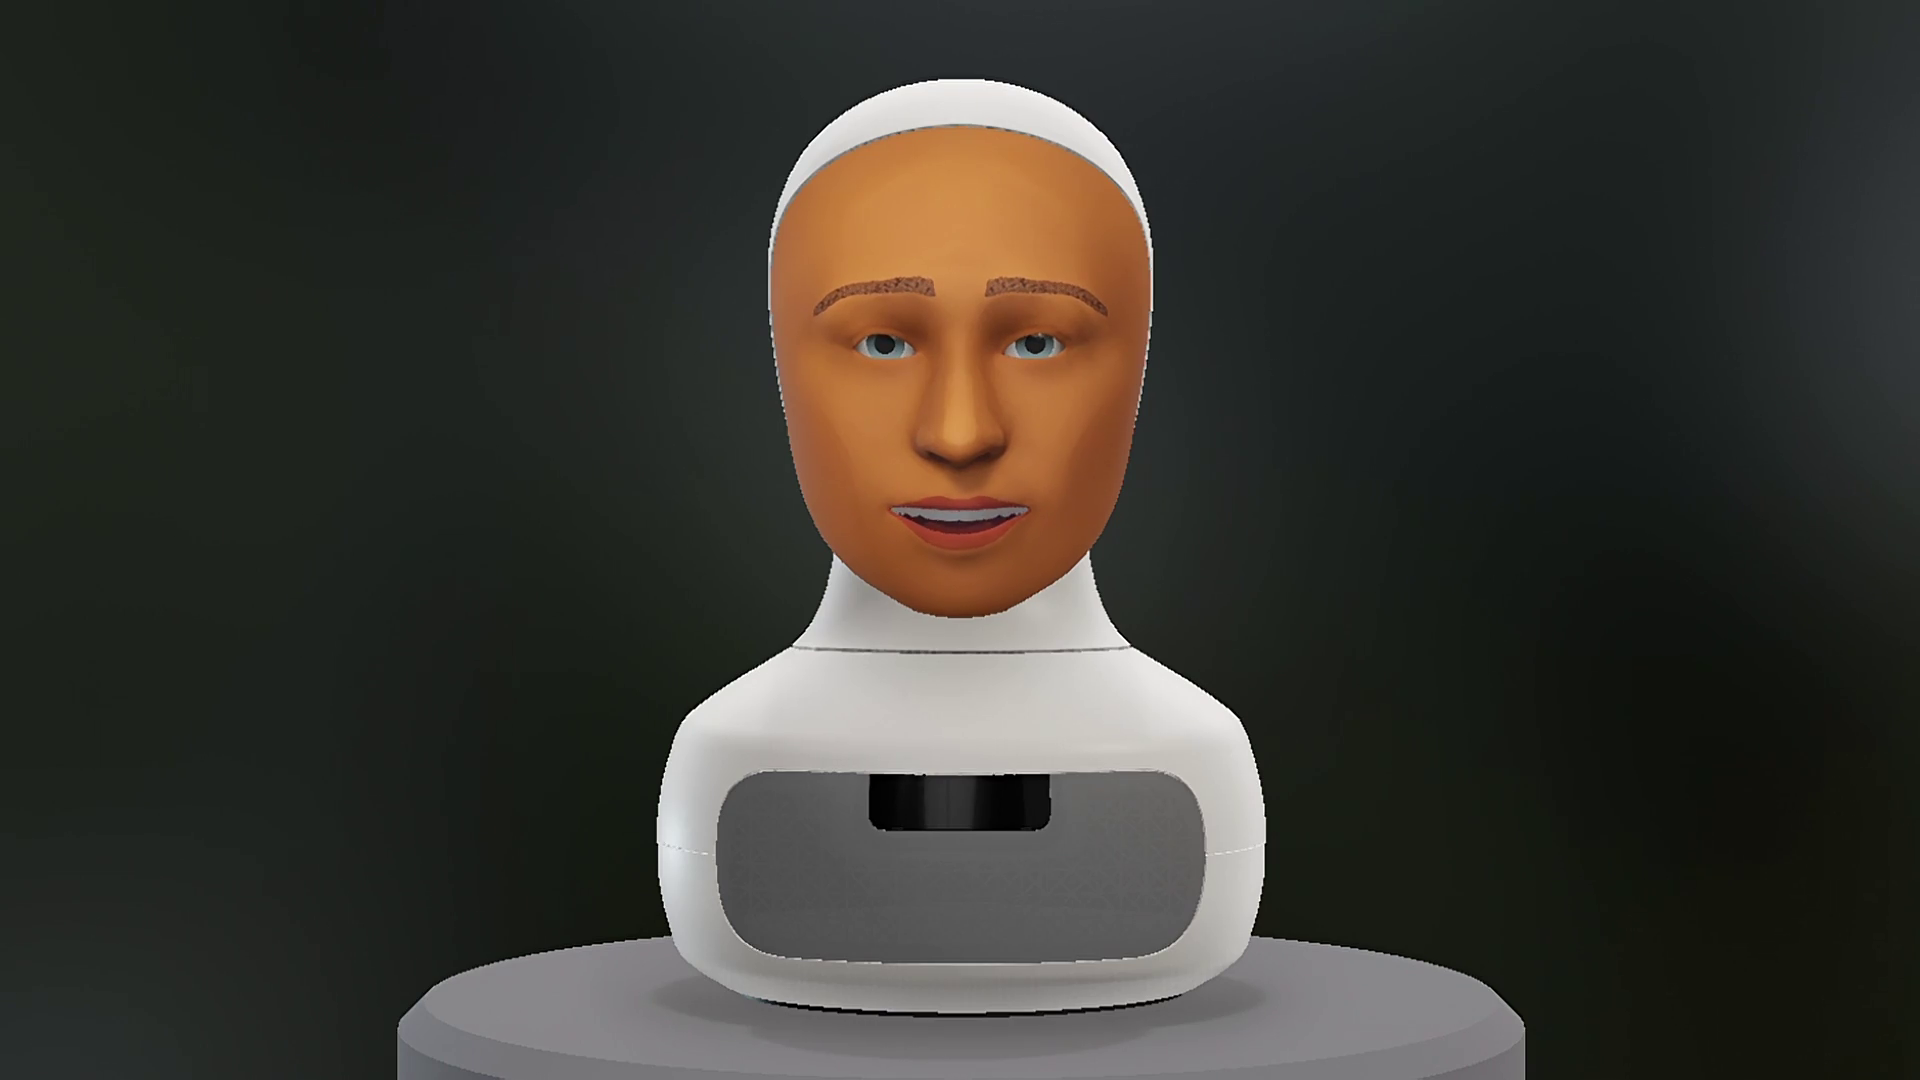
\includegraphics{figures/study_screenshot_1.png}
        \end{adjustbox}
        \begin{adjustbox}{max width=0.5\textwidth}
        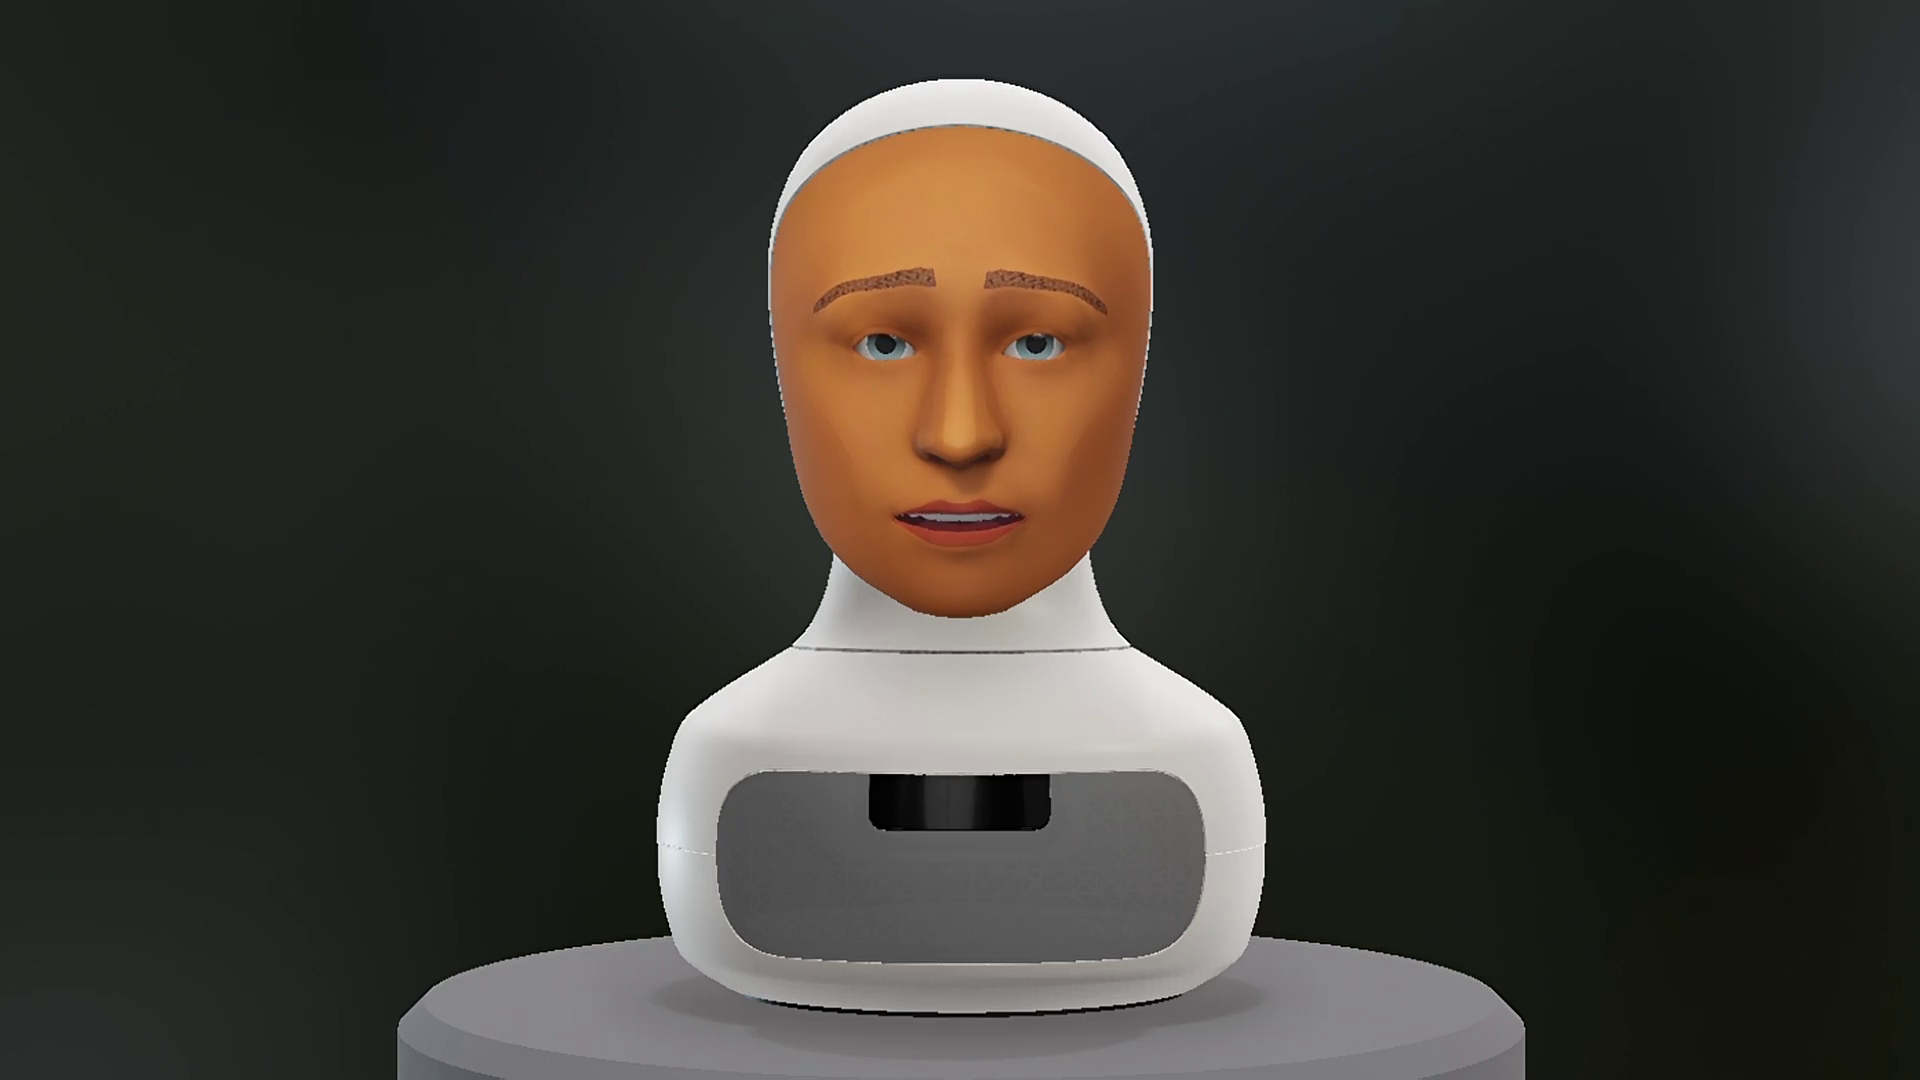
\includegraphics{figures/study_screenshot_2.png}
        \end{adjustbox}
    \end{adjustbox}
    \caption{Two screenshots of the videos used for the study.}
    \label{fig:study_screenshots}
\end{figure}

We used Prolific to recruit 40 men and 40 women (through its screening tools), 20 participants per condition (equally distributed across genders). Each participant in the study is initially asked to compile a short questionnaire to assess their personality (used to check for personality matching). The questionnaire has been extracted from the one used in the pilot (shown in \Cref{tab:pilot_survey}) where we removed the questions on fluency and the questions explicitly asking the introversion/extraversion. Each participant then watches a video with the robot animating the first introduction dialogue from the pilot (see \Cref{tab:dialogues}) and manifesting congruent emotional expressions (the video was available to re-watch at every step of the questionnaire). For a direct comparison with the pilot, the participant is first asked to rate the same questions in \Cref{tab:pilot_survey}, again, on a 7-point Likert scale. We also used questions from the Godspeed questionnaire~\cite{bartneck2009measurement} for the measures of Anthropomorphism, Likeability and Perceived Safety and questions of Warmth and Discomfort from the RoSAS questionnaire~\cite{carpinella2017robotic}, all presented on a 5-point Likert scale. We show these additional questions in \Cref{tab:study_survey}.

\begin{table}
    \centering
    \begin{adjustbox}{max width=\textwidth}
        \begin{tabular}{|p{0.3\textwidth}|p{0.3\textwidth}|p{0.4\textwidth}|}
        \hline
        Measure Low & Measure High & Origin \\
        \hline
        \hline
        Fake & Natural & Godspeed Anthropomorphism\\
        \hline
        Machine-like & Human-like & Godspeed Anthropomorphism\\
        \hline
        Unconscious & Conscious & Godspeed Anthropomorphism\\
        \hline
        Artificial & Lifelike & Godspeed Anthropomorphism\\
        \hline
        Moving rigidly& Moving elegantly & Godspeed Anthropomorphism\\
        \hline
        Dislikable & Likable & Godspeed Likeability\\
        \hline
        Unfriendly & Friendly & Godspeed Likeability\\
        \hline
        Unkind & Kind & Godspeed Likeability\\
        \hline
        Unpleasant & Pleasant & Godspeed Likeability\\
        \hline
        Awful & Nice & Godspeed Likeability\\
        \hline
        Anxious & Relaxed & Godspeed Perceived Safety\\
        \hline
        Calm & Agitated & Godspeed Perceived Safety\\
        \hline
        Quiescent & Surprised & Godspeed Perceived Safety\\
        \hline
        - & Happy & RoSAS Warmth \\
        \hline
        - & Feeling & RoSAS Warmth\\
        \hline
        - & Social & RoSAS Warmth\\
        \hline
        - & Organic & RoSAS Warmth\\
        \hline
        - & Compassionate & RoSAS Warmth\\
        \hline
        - & Emotional & RoSAS Warmth\\
        \hline
        - & Scary & RoSAS Discomfort\\
        \hline
        - & Strange & RoSAS Discomfort\\
        \hline
        - & Awkward & RoSAS Discomfort\\
        \hline
        - & Dangerous & RoSAS Discomfort\\
        \hline
        - & Awful & RoSAS Discomfort\\
        \hline
        - & Aggressive & RoSAS Discomfort\\
        \hline
        \end{tabular}
    \end{adjustbox}
    \caption{The questions used in the second study in addition to those in \Cref{tab:pilot_survey}. The participants were prompted with: ``Please indicate the extent you think the robot is...".}
    \label{tab:study_survey}
\end{table}

We use the combination of Godspeed Anthropomorphism and Perceived Safety, RoSAS Warmth and Discomfort as a proxy for uncanniness. We also use the questions from RoSAS Warmth as a measure of emotional expression.

We included in the survey different types of attention checks, 3 of them were among the questions, of the type ``click disagree/strongly agree for this question". We also asked each participant at the end what was the name of the robot and the topic of the dialogue. Participants could choose among 6 possibilities for each. The participants received a £1.50 compensation for completing the survey.
\subsection{Results}
Among the 80 recruited participants, we excluded 6 due to failed attention checks. The remaining population was composed of 38 women, 35 men and one that did not self-identified among our options (chose `other'). The average age is 28 ($M=28.11$, $SD=9.04$) and it is plotted in \Cref{fig:study_age}.
\begin{figure}
    \centering
    \begin{adjustbox}{max width=\textwidth}
        \includesvg{figures/study age} 
    \end{adjustbox}
    \caption{Distribution plot of the age of the participant in our final study.}
    \label{fig:study_age}
\end{figure}
18 participants reported being native speakers of English while 56 reported being ``Comfortable enough to understand English in most cases". Also, following our self-report questionnaire on personality, 44 participants were on the higher end of the extraversion trait (extroverts) while only 30 were on the lower end (introverts). 

All the statistical analysis that follows was made using the open-source software JASP~\cite{JASP2022}. The data collected and the analysis done are available under \href{https://github.com/alessioGalatolo/Furhat-Personality-and-Emotions/tree/main/study_data}{\mintinline{bash}{study_data}} in our \href{https://github.com/alessioGalatolo/Furhat-Personality-and-Emotions/}{GitHub Repository}.
\subsubsection{RQ2 - Manipulation check}
Our first analysis was aimed at verifying the correct manipulation of the personality in the dialogues i.e. the extroverted dialogue is perceived as significantly more extroverted than the introverted one. Similarly to what was done in the pilot, to compare the dialogues we only use the extraversion score which is an average of the introversion (reversed) and extraversion questions.

For each of our models, we run two independent samples tests, comparing their two versions of the dialogue. For STRAP, we used the Student t-test and discovered that the difference in extraversion is not significant ($t(34)=1.392, p=0.086$).

For GPT-3 we run two Mann-Whitney U tests due to the violation of the normality assumption (shown by a Shapiro-Wilk test, $W=0.898, p=0.044$ in the extroverted dialogues). GPT-3, similarly to STRAP, does not generate a significant difference between the two dialogues ($W=218.5, p=0.076$). However, plots relative to the extraversion, shown in \Cref{fig:study_personality}, still suggest that generally both introverted dialogues are perceived more introverted and the extroverted dialogues are perceived more extroverted.

\begin{figure}[ht]
    \centering
    \begin{adjustbox}{max width=\textwidth}
        \includesvg{figures/study extraversion box} 
    \end{adjustbox}
    \caption{Plots with the ascribed extraversion of the dialogues on a scale from 0 to 6.}
    \label{fig:study_personality}
\end{figure}

A subsequent Kruskal-Wallis test (done in the place of \gls{ANOVA} due to the violation of normality) including both models (therefore comparing only the extroverted dialogues against the introverted ones) revealed a significant difference in extraversion ($H(1) = 4.388, p=0.036$), confirmed by Dunn's post-hoc test ($p=0.018$).

\subsubsection{RQ2 - Difference in fluency and performance}
To answer the research questions that follow we did a series of independent samples \glspl{ANOVA} (or Kruskal-Wallis if the normality or equality of variance assumptions were violated) comparing the relevant measures across model and personality (introverted or extroverted dialogue).

A Kruskal-Wallis test revealed a significant difference in fluency across all conditions ($H(3)=27.509, p<0.001$), across the personality ($H(1)=5.124, p=0.024$) but not across models ($H(1)=2.998, p=0.083$). A post-hoc Dunn's test confirmed the extroverted dialogues to be ascribed more fluency than the introverted ones ($p=0.012$). %
% but also a significant difference across the models ($p=0.042$) where GPT-3 is rated to be more fluent than STRAP (\Cref{fig:study_rq2}). 
A Dunn's test comparison across all conditions also revealed GPT-3 extroverted dialogue to be significantly more fluent than STRAP introverted dialogue ($p=0.013$ using Bonferroni or Holm correction).

\begin{figure}[ht]
    \centering
    \begin{adjustbox}{max width=\textwidth}
        \begin{adjustbox}{max width=0.5\textwidth}
            \includesvg{figures/study fluency}
        \end{adjustbox}
        \begin{adjustbox}{max width=0.5\textwidth}
            \includesvg{figures/study performance} 
        \end{adjustbox}
    \end{adjustbox}
    \caption{Plots with the ascribed fluency of the dialogues (left) and the personality performance (right) on a scale from 0 to 6.}
    \label{fig:study_rq2}
\end{figure}
The same Kruskal-Wallis test was repeated for personality overall performance\footnote{Similarly to the pilot, the personality overall performance is computed by using both the introversion and extraversion measure i.e. it measures how much the introverted dialogue is introverted \textit{and} non-extroverted, vice-versa for the extroverted dialogue.}, revealing a significant difference across all conditions ($H(3)=27.509, p<0.001$), the different version of the dialogues ($H(1)=25.863,p<0.001$) but not across the models ($H(1)=0, p=1$). Again, a post-hoc Dunn's test reveals differences across the personality condition ($p<0.001$ with Holm or Bonferroni correction) with the extroverted dialogues performing better (\Cref{fig:study_rq2}) than the introverted ones.

In this context, both our models perform worse on generating introverted dialogues, this is reflected in the personality manifestation of each version where the introverted one fails to be `enough' introverted and is therefore closer to the extroverted one. Ideally, to have the biggest difference in personality manifestation between the two dialogues, the performance score should be of similar height for both version with the difference growing alongside the growth of the two scores.

\subsubsection{RQ2 - Emotional manifestation}
\Cref{fig:emotions_progression} shows the intensity of the emotions expressed by each version of the dialogue. This includes all emotions, although the major one manifested by each dialogue is joy. We see from the figure how the extroverted versions of each model generated higher intensity emotions.
\begin{figure}[ht]
    \centering
    \begin{adjustbox}{max width=\textwidth}
    \begin{tikzpicture}
      \begin{axis}[
        width=\textwidth,
        legend pos=south east,
        xlabel=Percentage of time,
        ylabel=Emotional intensity,
        xmin=0,
        xmax=100,
        ymax=1,]
        \addplot[smooth, mark=diamond, red] coordinates {(0.0, 0.5341728162020445) (12.5, 0.4362278562039137) (25.0, 0.441612197086215) (37.5, 0.6079319510608912) (50.0, 0.7309195045381784) (62.5, 0.4970747344195843) (75.0, 0.5603331277767817) (87.5, 0.7855380102992058) (100.0, 0.618270754814148)};
        
        \addplot[smooth, mark=x,blue] coordinates {(0.0, 0.7559357746504247) (8.333333333333332, 0.7422369509004056) (16.666666666666664, 0.9456846439279616) (25.0, 0.7944377241656184) (33.33333333333333, 0.7783088563010097) (41.66666666666667, 0.5726636657491326) (50.0, 0.6512421388179064) (58.333333333333336, 0.5428289333358407) (66.66666666666666, 0.6926554588135332) (75.0, 0.628594740992412) (83.33333333333334, 0.8201132810985049) (91.66666666666666, 0.7508709258399904) (100.0, 0.9867132259532809)};
        
        \addplot[smooth, mark=+, green] coordinates {(0.0, 0.3132602423429489) (14.285714285714285, 0.4374654879793525) (28.57142857142857, 0.43524916376918554) (42.857142857142854, 0.5768471544142812) (57.14285714285714, 0.5499829386826605) (71.42857142857143, 0.703336998509864) (85.71428571428571, 0.5567301898263395) (100.0, 0.9873079238459468)};
        
        \addplot[smooth, mark=o, yellow] coordinates {(0.0, 0.46999000012874603) (14.285714285714285, 0.37442733347415924) (28.57142857142857, 0.5857755434699357) (42.857142857142854, 0.7764073987491429) (57.14285714285714, 0.6398285110481083) (71.42857142857143, 0.8185165033986171) (85.71428571428571, 0.9805187443271279) (100.0, 0.9861666113138199)};
        \legend{GPT-3 Int, GPT-3 Ext, STRAP Int, STRAP Ext}
      \end{axis}
    \end{tikzpicture}
    \end{adjustbox}
    \caption{Progression of the emotional manifestation intensity throughout the dialogue.}
    \label{fig:emotions_progression}
\end{figure}
% \begin{figure}[ht]
%     \centering
%     \begin{adjustbox}{max width=\textwidth}
%     \begin{tikzpicture}
%       \begin{axis}[
%         width=\textwidth,
%         legend pos=south east,
%         xlabel=Percentage of time,
%         ylabel=Emotional intensity,
%         xmin=0,
%         xmax=100,
%         ymax=1,]
%         \addplot[smooth, red] coordinates {(0.0, 0.45067559694871306) (12.5, 0.31676380382850766) (25.0, 0.3116949914256111) (37.5, 0.49167057184968144) (50.0, 0.5756142182508484) (62.5, 0.3531339658657089) (75.0, 0.4500787576350073) (87.5, 0.6720835417509079) (100.0, 0.42015770077705383)};

%         \addplot[smooth, blue] coordinates {(0.0, 0.43065284157637507) (8.333333333333332, 0.42875762248877436) (16.666666666666664, 0.6300399523461238) (25.0, 0.6732458844780922) (33.33333333333333, 0.6305500129237771) (41.66666666666667, 0.42455831152619794) (50.0, 0.5098549423855729) (58.333333333333336, 0.36456771922530606) (66.66666666666666, 0.5478377303224988) (75.0, 0.541519439604599) (83.33333333333334, 0.7211091021696726) (91.66666666666666, 0.6158874481916428) (100.0, 0.9108569622039795)};
        
%         \addplot[smooth, green] coordinates {(0.0, 0.141730377683416) (14.285714285714285, 0.2897028198931366) (28.57142857142857, 0.29899660707451403) (42.857142857142854, 0.5188617438543588) (57.14285714285714, 0.5164278475567698) (71.42857142857143, 0.6678347463409106) (85.71428571428571, 0.5077189616858959) (100.0, 0.9159855246543884)};
        
%         \addplot[smooth, yellow] coordinates {(0.0, 0.27861216966994107) (14.285714285714285, 0.15421379660256207) (28.57142857142857, 0.3720185693819076) (42.857142857142854, 0.5562283147592098) (57.14285714285714, 0.5489891560282558) (71.42857142857143, 0.7285570601622263) (85.71428571428571, 0.9336391389369965) (100.0, 0.924099862575531)};

%         \legend{GPT-3 Int, GPT-3 Ext, STRAP Int, STRAP Ext}
%       \end{axis}
%     \end{tikzpicture}
%     \end{adjustbox}
%     \caption{Progression of the joy emotion manifestation intensity throughout the dialogue.}
%     \label{fig:joy_progression}
% \end{figure}

Using the data from the study, \gls{ANOVA} testing showed no significant differences across all conditions ($F(3, 69)=2.326, p=0.132$), personality ($p=0.448$) or model ($p=0.315$) in the emotional perception. However, a independent samples Student t-test with only STRAP results revealed its extroverted dialogue to be significantly more emotional than the introverted one (\Cref{fig:study_rq5}): $t(34)=1.906, p=0.033$.

\begin{figure}[ht]
    \centering
    \begin{adjustbox}{max width=\textwidth}
        \includesvg{figures/study emotion}
    \end{adjustbox}
    \caption{Plot with the ascribed RoSAS warmth measures as a proxy for emotional manifestation on a scale from 0 to 4.}
    \label{fig:study_rq5}
\end{figure}

\subsubsection{RQ3 - Perception of uncanniness}
A Kruskal-Wallis test on the uncanniness (\Cref{fig:study_rq3}) revealed no significant difference across all conditions ($H(3)=5.941, p=0.115$), across the personality condition ($H(1)=0.454, p=0.501$) or the model ($H(1)=3.078, p=0.079$). 
% However, a subsequent Dunn's test revealed the difference between the models to be significant ($p=0.04$) with STRAP being perceived more uncanny than GPT-3. A comparison across all conditions revealed close to significant results on GPT-3 introvert dialogue being less uncanny than STRAP introvert ($p=0.01$ with no correction, $p=0.059$ with Bonferroni or Holm correction).

\begin{figure}[ht]
    \centering
    \begin{adjustbox}{max width=\textwidth}
        \begin{adjustbox}{max width=0.5\textwidth}
            \includesvg{figures/study uncanniness} 
        \end{adjustbox}
        \begin{adjustbox}{max width=0.5\textwidth}
            \includesvg{figures/study anthropomorphism} 
        \end{adjustbox}
    \end{adjustbox}
    \caption{Plots with the ascribed uncanniness of the dialogues (left - lower is better) and the Godspeed Anthropomorphism (right - higher is better). Both are on a scale from 0 to 4.}
    \label{fig:study_rq3}
\end{figure}
As our uncanniness measure is a combination of different measures that may be perceived differently, we deemed relevant to also test each measure separately. The only measure that varies significantly across our conditions is the Godspeed Anthropomorphism\footnote{NB: The measure of Anthropomorphism is not on the same scale of uncanniness i.e. high anthropomorphism does not necessarily result in high uncanniness or vice-versa.} where the difference, tested with ANOVA, is only significant across model \textit{and} personality ($F(3, 69)=2.606, p=0.04$) and only close to significance across models only ($F(3, 69)=3.037, p=0.086$). In \Cref{fig:study_rq3} we can see how the extroverted dialogue from STRAP is very close to that of GPT-3 while the introverted version is quite lower. A pairwise post-hoc test using Tukey's correction confirmed GPT-3 introvert to be significantly higher than STRAP introvert ($p=0.047$).

The personality of the participant does not have any significant effect on the ascribed uncanniness (ANOVA, $F(7, 65)=0.504, p=0.480$).
\subsubsection{RQ4 - Likeability}
A Kruskal-Wallis test showed no significant difference in likeability neither across all the conditions ($H(3)=1.832, p=608$), the models ($H(1)=0.177, p=0.674$) or the personality ($H(1)=1.355, p=0.244$). We can see, in \Cref{fig:study_rq4}, how GPT-3 and the extroverted dialogues are ascribed slightly more likeability but not enough to represent statistical significance. 

\begin{figure}[ht]
    \centering
    \begin{adjustbox}{max width=\textwidth}
        \includesvg{figures/study likeability}
    \end{adjustbox}
    \caption{Plot with the ascribed Godspeed Likeability on a scale from 0 to 4.}
    \label{fig:study_rq4}
\end{figure}
The personality of the participant does not have any significant effect on the personality perception (Kruskal-Wallis, $H(7)=5.826, p=0.560$).

\chapter{Discussion}
\label{ch:discussion}
In this chapter, we summarise the most important results from this thesis and discuss their meaning and the consequences.
\section{Initial findings}
Our first discussion is mainly concerned with the technical findings and is generally not connected to any explicit research question. In this section, we comment on some results obtained during the development of the technical side of this work. Here, we also present some limitation of our models.
\subsection{Understanding personality from single sentences is hard}
In \Cref{sec:gan_classifier} we tested the personality classification from text using single sentences or multiple ones. The only meaningful results we got were when testing groups of sentences from the same person. On the other hand, classifying single sentences, gave close to random results. It is our opinion that future works trying to classify the personality from text should gather more than a few sentences from a single person and base the classification on all of those. It is also important to remark how the classification was never the primary goal of this thesis but has been explored as a result of the architecture of the first model tested. 

Future works might look to further develop personality classification in order to extend our pipeline to robot personality generation being based on that of the user.
\subsection{Bigger models are better at extending sentences but not at paraphrasing}
In \Cref{ch:methods} we reported the results on the three proposed methods varying on the number of parameters. Starting from the model with the lowest amount, the GAN-based method, we can notice how it is completely unable to successfully complete the task. While the method has been proved successful in other domains, such as the sentiment transfer~\cite{yang2018unsupervised}, it was not powerful enough to be applied to ours. Reasons for this can be found in the nature itself of the task. To change the sentiment of a sentence it is enough to understand which words bring the positive/negative attribution and swap them with their antonyms. However, the same reasoning cannot be applied when trying to transfer the personality, where the changes are a lot more subtle and require a better understanding of language and how it can be manipulated without altering the meaning of a sentence.

The other two models seemed to be behaving better, at least in terms of fluency of the sentences they were transferring. If we directly compare the two we can see how STRAP mostly tries to shape the personality by paraphrasing the sentence, changing the wording and the length of the sentence. GPT-3 rarely does any changes to the original sentences but the personality manifestation mainly comes from added sentences. These added sentences are very well placed and integrate naturally into the dialogue but also help providing great insight into the person (robot) who is talking.

\section{Research questions answered}
In the next section, we will be concerned with the discussion of the results from our user studies and how they can be used to answer the research questions initially formulated (see \Cref{sec:rqs}).

\subsection{Personality manifestation depends on the topic} 
From the pilot results, we can confirm that these automated models are able to work in some contexts (although not much in others). Personality manifestation and its perception are really hard tasks both for humans and automated methods and not all contexts permit the correct reception of it. Further, when the interaction is limited to only a single dialogue, the correct reception of the personality highly depends on the topic of that dialogue. A more `personal' dialogue, such as an introduction or when talking about oneself has a much greater manifestation of personality than a dialogue about an objective topic such as that on humanities. We can even report having a harder time making the hand-crafted version of the last two dialogues than for the first, the introduction dialogue. Even though the hand-crafted versions of the last two dialogues still report the correct perception of the aimed personality, we speculate this may only be due to a very high exaggeration of the personality manifestation that would not probably happen in real-world scenarios.

Let us also compare the performance of the two models overall and in terms of fluency. While the fluency score is significantly higher for GPT-3, which almost reaches the performance of our hand-crafted versions, the overall performance is very close between the two. We have to consider, however, that the outputs of STRAP have been manually filtered to increase fluency. If dropping this filtering we would probably also have to drop the top-p value by at least 0.1 or 0.2 to remove the manifestation of less natural or badly paraphrased sentences. We speculate that this would also reduce the manifestation of the personality, at least to some extent.

This answers our first research question on the relation of size and performance of language models. Despite GPT-3 being much larger than STRAP, the performance is comparable, with GPT-3 having a bigger edge only in the fluency measure.

\subsection{Personality manifestation in robotic speech is (almost) significant}
To begin our follow-up study, we checked that our manipulation of the personality was successful. Our tests indicate that the difference in extraversion is not statistically significant. However, given the closeness to a significant value, our results on the pilot and the qualitative results on the study we hypothesise that our manipulation checks were successful nonetheless. Our sample size was fairly small and it is possible that a more subtle change in personality may require a higher number of participants to reach statistical significance.

If we try to examine where our models could improve by looking at their performance, we can see how both models struggle quite a bit with the introverted dialogue. While they achieve better results in the extroverted one. Reasons for this may be due to the intrinsic way in which a dialogue can appear more introverted rather than extroverted. If we think of some of the manipulations that can be made to a dialogue to make it seems more extroverted (see \Cref{sec:hand_crafted}), there is `being more talkative'~\cite{pennebaker1999linguistic, furnham1990language}, `have less complex sentence'~\cite{furnham1990language}, etc. Both of which are much harder to apply in the introversion case. When making a dialogue more talkative, one can repeat some of the content, or add new one that closely relates to the dialogue. Making it less talkative is not a mere removal of content because that would change radically the meaning of the sentence, one should understand the key concept in a dialogue and try to remove anything else, which is much harder. Similar reasoning can be applied to complexity, where making a less complex sentence is easier than making a more complex one.

\subsection{GPT-3 is more fluent but not better performing than STRAP}
Our results in RQ2, show how there is a significant difference in fluency across the personality condition with the extroverted dialogues being perceived as more fluent. This is somewhat expected as an extroverted personality is generally more talkative, use less complex sentences and fewer hedges which may be perceived as also being more fluent. Also, STRAP is generally ascribed less fluency than GPT-3 (although not significant), a factor that combined with the difference between personality makes GPT-3 extrovert significantly more fluent than STRAP introvert.

If we consider the performance, on the other hand, there is absolutely no difference between the two models, suggesting the advantage of GPT-3 in the task mostly lies in its fluency. This goes against our initial findings in the pilot where we could see a bigger difference between the two suggesting that multi-modal speech delivery has helped closing the gap between the two (contrary to what we hypothesised in H2). 

Further, plots for uncanniness show how there is a difference in perception between the models, at least for some of their generation. However, the difference is not enough to represent statistical significance. Reasons for this can be multiple, ranging from the (short) duration of the interaction to the too small changes between one robot and the other to be perceived by the participant. This also goes against our hypothesis for our third research question where we expected fluency to have an effect on uncanniness as it should reflect on how `human' and `natural' the robot is perceived. 

\subsection{Likeability and personality matching effects are too little to measure}
Our results on likeability and personality matching do not confirm our hypothesis that personality matching improves the interaction and the likeability of the robot. We explain these results with the relatively short duration of our experiment. In fact, to register a positive difference (or any difference at all), the user would need to better understand the robot, its purpose, or how it behaves. Possibly through a more active session that involves the user directly.
% \section{Uncanniness correlates to ...}

\subsection{Emotional manifestation depends on personality (but maybe not)}
We have shown, in the previous chapter, how text of different personality triggers a different emotional manifestation with the extroverted ones triggering a higher intensity in emotions confirming our hypothesis H2. However, our results suggest a significant difference only in the case of STRAP. 

However, in this experiment, many could be the confounding factors. The perceived emotions could be different due to the slightly different content of the dialogue or due to other differences that should not play a role. Further, while STRAP extroverted dialogue has been perceived as more emotional, the opposite is true for GPT-3 even though the intensity is generally higher for GPT-3 extrovert. We, therefore, think that to better back our claim that a change in textual personality is enough to manifest significantly different emotions, more experiments with different dialogues in different contexts are needed.

\chapter{Conclusions}
\label{ch:conclusions}
This thesis explored different approaches to automatic processing of text to convey different personalities, with particular attention to the extraversion trait. We proposed the use of three different language models varying in the size of their architecture: a GAN-based model, STRAP and GPT-3. Our initial results suggest that our smallest model is not able to successfully complete the task. The other two models perform very similarly in terms of personality manipulation but the largest model (GPT-3) outperforms the other (STRAP) in terms of fluency. 

We showed, through an online pilot study how different kinds of dialogues provided only as text can be shaped to convey a personality trait rather than another. We confirmed that the difference is perceptible by people through hand-crafted versions of the dialogues which have always been correctly ascribed the aimed personality. The performance of our automated models, STRAP and GPT-3, varies depending on the type of dialogue. We do not deem this a limitation of our models but rather a limitation of how much a dialogue can change to convey a personality.
% Stressing too much on manifesting the personality only through language (ignoring prosody, body movements, etc.) can end up in unnatural behaviour where the robot may be perceived to be particularly uncanny.

After comparing the performance of our models, we worked on incorporating the dialogues into the social robot Furhat. We also used a method to extract emotions from the dialogues' text to be then manifested through the facial expressions of the robot. We tested through a second online study the perception of the robot when animating those dialogues with appropriate emotions.

Our second study revealed how the dialogues were generally ascribed the correct personality but how this was not statistically significant (possibly due to small sample size). Our second study confirmed how STRAP is sometimes perceived as less fluent than GPT-3 (significant) but how they perform very similarly. We found out that both models perform better when generating an extroverted dialogue than an introverted one (significant). The dialogues from STRAP made for a robot that is perceived slightly more uncanny than GPT-3 (not significant) although, much of the difference is due to the introverted dialogue from STRAP.

We did not record any (significant) difference in the likeability of the robot. Similarly, we did not find that the personality of the participant had any influence on the perception of the robot. This goes against other findings in the literature~\cite{andrist2015look, esterwood2021birds, andriella2020have}, but likely links to the short length of our participant-robot interactions and the video-based nature of our study. Finally, although both models trigger a bigger emotional manifestation in the extroverted version of the dialogue, only STRAP resulted in a significant difference in the amount of emotion generated for the introvert versus extrovert robot dialogue - something that likely contributed to increased differences in perception of those versions of the robot and therefore worth investigating further in future work on automatic personality generation and expression. 
\section{Future work and limitations}
Points for improvement and extension in this work are countless as the topics addressed are very broad and pose many, currently unsolved, problems.

Starting from the datasets, these impose a big limitation in terms of the performance achievable. A more ``personality-expressive" dataset like the PERSONAGE one can help to create a more congruent model. However, the PERSONAGE dataset itself cannot be used directly due to its limited size. The MBTI dataset is very big but also very ineffective (according to our testing) due to its limited scope and the very informal setting in which it was collected. The Essays dataset is very expressive in the personality, given its very personal nature but it is very limited in the topic and in its size. Furthermore, both MBTI and Essays contain `made up' words that worse the performance of any model they are trained on. A way of gathering a dataset that may improve the performance of the methods proposed could be labelling a \gls{NLP} dataset using a personality classification model, given that its performance reaches the level needed for such a process.

When comparing the performance of our two best language models, STRAP and GPT-3, we observed how they have two different ways of processing a text to express personality. STRAP heavily relies on changing the wording and paraphrasing while GPT-3 mostly adds/removes content from the dialogues. Future works could explore the use of these two models in combination to achieve even better performances.

Also, when testing GPT-3 we only tried a prompt-based approach with zero or one-shot learning. Compared to our STRAP approach where we took another language model and fine-tuned it for our tasks. As it is also claimed in \href{https://openai.com/blog/customized-gpt-3/}{openAI blog}\footnote{\url{https://openai.com/blog/customized-gpt-3/}}, this approach is preferable and often yields better performance than a prompt-based one.

As we outlined in many parts of this manuscript, we only focused our work on the extraversion trait as it is considered to be easier to manifest through language and has more literature~\cite{pennebaker1999linguistic, furnham1990language, thorne1987press, heylighen2002variation, dewaele1999extraversion} (especially in \gls{HRI}~\cite{aly2013model, andriella2020have, moshkina2011tame}) supporting it. We believe, however, that our proposed methods should still work even on different personality traits. For STRAP, we can imagine the creation of a pipeline of 5 models to create the wanted personality (one for each trait). A similar strategy can also be applied to GPT-3. We can expect, when expanding to the whole personality spectrum, that the manifestation of some traits would be more evident depending on the context. With some traits having a bigger impact on dialogues where others have little to no impact. For example, we can expect, for our dialogue on humanities, that the conscientiousness or openness traits to have a much bigger impact than the extraversion one.

When it comes to the \gls{HRI} side of this work, it probably would benefit from a more in-depth and in-person study where one can accurately measure the difference in likeability of the robot and the possible effect of personality matching on the interaction. However, when integrating these methods into a conversational robot, it has to be considered that in this work we have always pregenerated the dialogues used as well as their different personality versions. Starting from the latter, our experiments revealed that GPT-3 is much faster than STRAP in outputting the desired personality-adapted dialogue, mostly due to the more powerful servers used. This implies that while GPT-3 is ready to be used in a dynamic environment where the response of the robot can be computed on demand, STRAP needs further optimisation or a stronger server base. Another limitation of this work that could be explored in future development is the lack of an automated method for generating the base dialogues. In fact, our pipeline presented at the very beginning of this work (see \Cref{fig:system_flow}) start with a given dialogue.

\cleardoublepage
% Print the bibliography (and make it appear in the table of contents)
\renewcommand{\bibname}{References}
\printbibliography[heading=bibintoc]

\cleardoublepage
\appendix
% \renewcommand{\chaptermark}[1]{\markboth{Appendix \thechapter\relax:\thinspace\relax#1}{}}
\chapter{STRAP extensive results}
\label{app:strap_complete_results}
The appendix presents extensive results with the \gls{STRAP} model. \Cref{tab:strap_n_essays_extensive} and \Cref{tab:strap_np_essays_extensive} shows results on the Essays dataset for nucleus and nucleus paraphrase, respectively. \Cref{tab:strap_n_mbti_extensive} and \Cref{tab:strap_np_mbti_extensive} shows results on the MBTI dataset for nucleus and nucleus paraphrase.
\begin{table}
    \centering
    \begin{adjustbox}{max width=\textwidth}
        \begin{tabular}{|p{0.05\textwidth}|p{0.05\textwidth}|p{0.40\textwidth}|p{0.40\textwidth}|}
        \hline
        Top-p & Personality & Input & Output \\
        \hline
        \hline
        0.4 & I & I come from Stockholm, in Sweden where I was created by a company called Furhat Robotics and programmed by researchers from KTH University. & I come from svenskan, in svensk, where I was created by a company called Furhat Robotics and programmed by researchers from KTH University. \\
        \hline
        0.7 & I & I come from Stockholm, in Sweden where I was created by a company called Furhat Robotics and programmed by researchers from KTH University. & My parents were born in Stockholm, in Sweden where I was born out of a company called Furhat Robotics and programmed by researchers from KTH University. \\
        \hline
        1 & E & I come from Stockholm, in Sweden where I was created by a company called Furhat Robotics and programmed by researchers from KTH University. & Furhat Robotics is the parent company and programmer of part of my freaking year in ut and made me come from outside then to my home in spanish where I are already starting off.\\
        \hline
        0.4 & I & I am always here for you, and I will never get tired of your company. & I always have a place to go and always will be here for you and never get tired of your company. \\
        \hline
        0.8 & E & I am always here for you, and I will never get tired of your company. & The only reason I always stay here is to get you and I will never get tired of your company. \\
        \hline
        0.9 & E & I look forward to getting to know you better and to helping you in any way I can. & It is my dream come true to get to know you better and to help you in any way I can. \\
        \hline
        0.7 & I & Before we start, I would like to get to know you better, so I am going to ask you some questions. & I think that I should go and get to know you better before we start this. \\
        \hline
        0.7 & E & Before we start, I would like to get to know you better, so I am going to ask you some questions. & I would like to get to know you better before we start this and that is ok because I will ask some questions here.\\
        \hline
        \end{tabular}
    \end{adjustbox}
    \caption{Extensive results of STRAP trained on the Essays dataset. The output mode is nucleus.}
    \label{tab:strap_n_essays_extensive}
\end{table}
\begin{table}
    \centering
    \begin{adjustbox}{max width=\textwidth}
        \begin{tabular}{|p{0.05\textwidth}|p{0.05\textwidth}|p{0.40\textwidth}|p{0.40\textwidth}|}
        \hline
        Top-p & Personality & Input & Output \\
        \hline
        \hline
        0.5 & I & I am always here for you, and I will never get tired of your company. & I will always be here for you and never let you down .\\
        \hline
        0.6 & E & I was designed to help you with whatever you need, whether it is keeping you company or helping you in everyday tasks. & I am designed to help you with whatever is needed to stay on top of things in life and whether it is keeping you company or helping you in everyday tasks. \\
        \hline
        0.8 & I & I was designed to help you with whatever you need, whether it is keeping you company or helping you in everyday tasks. & I have a purpose that I can serve to help you with any assignment you may have and whether it be keeping you company or helping you in everyday tasks.\\
        \hline
        0.7 & I & As you know, today we are going to do some exercise, do you enjoy exercising? & I mean we're going to do some exercises today you know?\\
        \hline
        0.9 & E & I am pleased to meet you and I am looking forward to working together. & Speaking of working with you I am so glad to be able to meet you and I am looking forward to working with you.\\
        \hline
        1 & I & Before we start, I would like to get to know you better, so I am going to ask you some questions. & I wish I wasn't here because I supposed to find out later that I should've gone ahead and done.\\
        \hline
        0.6 & I & It is a broad field that covers a lot of ground, but there are a few key ideas that are essential to understanding humanities. & I think the humanities are a broad field but there are some key notions that are essential to understanding the humanities .\\
        \hline
        0.6 & E & Second, humanities is about interpretation. This means that there is no one right answer to any question in humanities. & Second philosophy about interpretation is what I mean by the humanities. That is why in humanities there is no right answer.\\
        \hline
        \end{tabular}
    \end{adjustbox}
    \caption{Extensive results of STRAP trained on the Essays dataset. The output mode is nucleus paraphrase.}
    \label{tab:strap_np_essays_extensive}
\end{table}
\begin{table}
    \centering
    \begin{adjustbox}{max width=\textwidth}
        \begin{tabular}{|p{0.05\textwidth}|p{0.05\textwidth}|p{0.40\textwidth}|p{0.40\textwidth}|}
        \hline
        Top-p & Personality & Input & Output \\
        \hline
        \hline
        1 & E & I am pleased to meet you and I am looking forward to working together. & You flustered me and I walked out smiling and I was very pleased receiving good news Just doing it together.\\
        \hline
        0.4 & E & As you know, today we are going to do some exercise, do you enjoy exercising? & As you know today we will do some exercise in the gym and do some exercise on your body? \\
        \hline
        0.5 & I & As you know, today we are going to do some exercise, do you enjoy exercising? & Do you enjoy Do you enjoy exercising today? \\
        \hline
        0.9 & I & I am here to talk to you about humanities. & Lol I am here for talking sciences.\\
        \hline
        0.8 & E & This means that the field is constantly evolving as new evidence and new interpretations are discovered & I think this means that the fields will constantly evolve as new evidence and new interpretations come to light.\\
        \hline
        0.9 & E & They must also be able to listen to and understand the ideas of others. & This is in part because the egos of others are so different from mine so they need to learn the ideas behind the others.\\
        \hline
        0.7 & I & I was designed to help you with whatever you need, whether it is keeping you company or helping you in everyday tasks. & I was made for you to help whatever you need most, whether it be keeping your company or helping you in everyday tasks.\\
        \hline
        0.7 & I & Before we start, I would like to get to know you better, so I am going to ask you some questions. & I think that I should go and get to know you better before we start this. \\
        \hline
        0.7 & E & Before we start, I would like to get to know you better, so I am going to ask you some questions. & I would like to get to know you better before we start this and that is ok because I will ask some questions here.\\
        \hline
        \end{tabular}
    \end{adjustbox}
    \caption{Extensive results of STRAP trained on the MBTI dataset. The output mode is nucleus.}
    \label{tab:strap_n_mbti_extensive}
\end{table}
\begin{table}
    \centering
    \begin{adjustbox}{max width=\textwidth}
        \begin{tabular}{|p{0.05\textwidth}|p{0.05\textwidth}|p{0.40\textwidth}|p{0.40\textwidth}|}
        \hline
        Top-p & Personality & Input & Output \\
        \hline
        \hline
        0.6 & I & I am always here for you, and I will never get tired of your company. I look forward to getting to know you better and to helping you in any way I can. & You will always be here for me and I will never be tired of you. I can't imagine a better way to understand you and help you.\\
        \hline
        0.7 & E & I come from Stockholm, in Sweden where I was created by a company called Furhat Robotics and programmed by researchers from KTH University. & I am from Stockholm, where I created a company called Furhat Robotics and programmed by scientists from KTH University to assemble an automated version of the Idris robot.\\
        \hline
        0.7 & E & I was designed to help you with whatever you need, whether it is keeping you company or helping you in everyday tasks. & I feel like my Design team is designed to help you with what you need and whether it is keeping you company or helping you in everyday tasks.\\
        \hline
        0.9 & I & My developers have also programmed me with sophisticated methods for recognising you so that I can always be awake when you need me but if you do not wish to have this feature I can always turn it off for you. & I also learned you were intelligent in a way that can be understood at the same time but if you do not want to it can go and walk in.\\
        \hline
        0.9 & E & I am always here for you, and I will never get tired of your company. & I'll always be there for you. And I won't wish it on your shoulder just because you have such a stupid sort of ability like.\\
        \hline
        0.8 & I & I am pleased to meet you and I am looking forward to working together. & I like meeting you and I am very excited to work with you. \\
        \hline
        0.8 & E & I am pleased to meet you and I am looking forward to working together. & I love meeting you and am looking forward to working with you in terms of. \\
        \hline
        0.8 & I & How do you feel about being here today? & Why does it even happen today? \\
        \hline
        1 & E & Great, I am glad to hear that! I am sure you will enjoy the session. & Dislike ya haha haha i could kinda agree with this anyway.\\
        \hline
        \end{tabular}
    \end{adjustbox}
    \caption{Extensive results of STRAP trained on the MBTI dataset. The output mode is nucleus paraphrase.}
    \label{tab:strap_np_mbti_extensive}
\end{table}
\chapter{Complete dialogues}
\section{GPT-3 generated dialogues}
\label{app:gpt3_intro_generation}
Our choice of the dialogues for the pilot study was aided by GPT-3. To generate the introduction dialogue we first used the prompt: ``This is a long introduction from a companion robot" receiveing the following output:
\begin{quote}
    My name is robot and I am here to be your companion. I will be with you through your ups and downs, and I will never leave your side. I know what you are feeling because I can read your emotions. I will be your best friend, and I will always be here for you.
\end{quote}
We then tried with ``This is a long introduction from a verbose talkative companion robot", resulting in:
\begin{quote}
    Welcome! My name is J.A.R.V.I.S. and I am your very own personal assistant robot! I am here to help you with whatever you need, whether it's keeping you company or helping you with your daily tasks. I am always here for you and I will never tire of helping you out. Thank you for choosing me as your companion robot!
\end{quote}
Finally we tried ``This is a long introduction from a verbose talkative companion robot" with top-p=0.67, resulting in:
\begin{quote}
    My name is Snickers and I am your new robotic companion! I was designed to provide you with companionship and to help you with your everyday tasks. I am equipped with a variety of sensors and cameras that allow me to see and hear what you are doing, and I also have a built-in GPS system so that I can always find my way back to you. I am always here for you, and I will never tire of your company. I look forward to getting to know you better and to helping you in any way I can. Thank you for choosing me as your companion.
\end{quote}
Our final introduction dialogue was created by merging these dialogues and by integrating new sentences.

The dialogue on humanities was entirely generated by GPT-3 with the prompt ``This is a verbose companion robot talking about humanities", resulting in:
\begin{quote}
    Hi, I am your verbose companion robot. I am here to talk to you about humanities. Humanities is the study of human culture, including history, literature, philosophy, and art. It is a broad field that covers a lot of ground, but there are a few key ideas that are essential to understanding humanities. First, humanities is about understanding the human condition. This includes understanding the way humans interact with each other and their environment. It also involves understanding the human past and how it has shaped the present. Second, humanities is about interpretation. This means that there is no one right answer to any question in humanities. Instead, scholars must use their critical thinking skills to interpret evidence and come to their own conclusions. Third, humanities is about communication. This means that scholars must be able to communicate their ideas clearly and persuasively. They must also be able to listen to and understand the ideas of others. Finally, humanities is about change. This means that the field is constantly evolving as new evidence and new interpretations are discovered. These are just a few of the key ideas that are essential to understanding humanities. If you want to learn more, there are many great resources available.
\end{quote}
\section{Other hand-crafted dialogues}
\label{app:hand_crafted}
We report in \Cref{tab:other_hand_crafted_2} and \Cref{tab:other_hand_crafted_3} the hand-crafted versions of second and third dialogue, respectively, used in the pilot study. Similarly to \Cref{tab:hand_crafted} we highlight in \textit{italics} the content changes, \sout{strike-through} the removed content and add as superscript the changes we did among those listed in \Cref{sec:hand_crafted} and conveniently re-summarised in \Cref{tab:hand_crafted_manipulations_app}.
\begin{table}
    \centering
    \begin{adjustbox}{max width=\textwidth}
        \begin{tabular}{|p{0.1\textwidth}|p{0.25\textwidth}|p{0.25\textwidth}|p{0.5\textwidth}|}
        \hline
        Number & Introvert & Extrovert & Manipulation \\
        \hline
        \hline
        1 & Less & More & talkative (more content and repetitions)\\
        \hline
        2 & Less & More & positive (focus on positive aspects, leave behind the negative ones)\\
        \hline
        3 & Less & More & subject implicit\\
        \hline
        4 & Less & More & self-referencing\\
        \hline
        5 & More & Less & complex\\
        \hline
        6 & High & Low & in number of hedges\\
        \hline
        7 & High & Low & in content negation\\
        \hline
        8 & More & Less & rich in vocabulary\\
        \hline
        \end{tabular}
    \end{adjustbox}
    \caption{List of possible manipulations of a dialogue to express different personalities.}
    \label{tab:hand_crafted_manipulations_app}
\end{table}
\begin{table}
    \centering
    \begin{adjustbox}{max width=\textwidth}
        \begin{tabular}{|p{0.5\textwidth}|p{0.5\textwidth}|}
        \hline
        Introvert & Extrovert \\
        \hline
        \hline
        \textbf{A:} I am pleased to meet you and \sout{I am looking forward to} \textit{start}$^1$ working together. Before we start, \sout{I would like to} \textit{perhaps I should}$^{2,6}$ get to know you better, so I am going to ask you some questions. How do you feel about being here today?\newline
        \textbf{B:} (...)\newline
        \textbf{A:} Great.\sout{, I am glad to hear that!}$^1$ \sout{I am sure} \textit{I think that}$^6$ you will enjoy the session. And how do you feel about working with me?\newline
        \textbf{B:} (...)\newline
        \textbf{A:} \sout{That is good to hear,} \textit{It seems that}$^6$ we will definitely have fun together today then. \sout{As you know,} Today we are going to do some exercise, do you enjoy exercising? \newline
        \textbf{B:} (...)\newline
        \textbf{A:} That makes sense, this session \sout{will be easy} \textit{won't be difficult}$^7$ for you then.
        &
        \textbf{A:} \sout{I am pleased} \textit{It's nice}$^{3,5}$ to meet you and \sout{I am looking forward to working together} \textit{I can't wait to start!}$^{2,5}$. \sout{Before we start, I would like to get to know you better, so I am going to ask you some questions} \textit{Let me ask you some questions first, so that I know you better before we begin}$^5$. How do you feel about being here today?\newline
        \textbf{B:} (...)\newline
        \textbf{A:} Great, I am \sout{glad} \textit{happy}$^8$ to hear that! I am sure you will enjoy the session. \textit{I am looking forward to working together}$^1$, how do you feel about working with me?\newline
        \textbf{B:} (...)\newline
        \textbf{A:} That is good to hear, we will definitely have fun together today then. \textit{I am sure you will enjoy the session}$^1$. As you know, today we are going to do some exercise. \textit{I think it's good to exercise,}$^{1,2,4}$ do you enjoy exercising? \newline
        \textbf{B:} (...)\newline
        \textbf{A:} \sout{That makes sense,} \textit{I am glad to hear that!}$^2$ This \sout{session} \textit{one}$^3$ will be easy for you then.\\
        \hline
        \end{tabular}
    \end{adjustbox}
    \caption{The manipulation done to the second dialogue to convey an extravert or introvert personality.}
    \label{tab:other_hand_crafted_2}
\end{table}
\begin{table}
    \centering
    \begin{adjustbox}{max width=\textwidth}
        \begin{tabular}{|p{0.5\textwidth}|p{0.5\textwidth}|}
        \hline
        Introvert & Extrovert \\
        \hline
        \hline
        I am here to talk to you about humanities. Humanities is \textit{concerned with}$^5$ the study of human culture, including history, literature, philosophy, and art. \sout{It is a broad field that covers a lot of ground, but}$^1$ \textit{I think that}$^6$ there are a few key ideas that are essential to understanding humanities. First, humanities is about understanding the human condition. This includes understanding the way humans interact with each other and their environment. It also involves understanding the human past and how it has shaped the present. Second, humanities is about interpretation. \sout{This means that there is no one right answer to any question in humanities. Instead,}$^1$ Scholars must use their critical thinking skills to interpret evidence and come to their own conclusions. Third, humanities is about communication. This means that \sout{scholars} \textit{academics}$^8$ must \sout{be able to communicate their ideas clearly and persuasively} \textit{not communicate their ideas in complex ways}$^7$. They must also be able to listen to and understand the ideas of others. Finally, humanities is about change. This means that the field is constantly evolving as new evidence and new interpretations are discovered. \sout{These are just a few of the key ideas that are essential to understanding humanities}$^1$. If you want to \sout{learn more} \textit{deepen your knowledge}$^8$, \sout{there are many great resources available} \textit{many resources are available out there}$^3$.
        &
        I am here to talk to you about humanities. \textit{I love the humanities}$^4$! \sout{Humanities is the study} \textit{It's about studying}$^3$ of human culture, including history, literature, philosophy, and art. It is a broad field that covers a lot \sout{of ground}$^8$, but there are a few key ideas that are essential to understanding humanities. First, humanities is about understanding the human condition. This includes understanding the way humans interact with each other and \sout{their environment} \textit{what surrounds them}$^8$. It also involves understanding the human past and how it has shaped the present. Second, humanities is about interpretation. This means that there is no one right answer to any question in humanities. Instead, \sout{scholars must use their} critical thinking skills \textit{are needed}$^3$ to interpret evidence and come to \sout{their own} conclusions. Third, humanities is about communication. \textit{Personally, I really like talking to people but}$^4$ \sout{This means that scholars} \textit{those in the field}$^{3,8}$ must be able to communicate their ideas \sout{clearly and persuasively} \textit{in a clear and persuasive way}$^5$. They must also be able to listen to and understand the ideas of others. Finally, humanities is about change. This means that the field is constantly evolving as new evidence and new interpretations are discovered. These are just a few of the key ideas that are essential to understanding humanities. If you want to learn more, there are many great resources available \textit{and I can definitely help you with that}$^4$!\\
        \hline
        \end{tabular}
    \end{adjustbox}
    \caption{The manipulation done to the third dialogue to convey an extravert or introvert personality.}
    \label{tab:other_hand_crafted_3}
\end{table}
%% The following label is necessary for computing the last page number of the body of the report to include in the "For DIVA" information
\label{pg:lastPageofMainmatter}

\clearpage
\kthbackcover
% \fancyhead{}  % Do not use header on this extra page or pages
% \section*{€€€€ For DIVA €€€€}
% \fancyhead{}  % Do not use header on this extra page or pages
% \divainfo{pg:lastPageofPreface}{pg:lastPageofMainmatter}
% \fancyhead{}  % Do not use header on this extra page or pages
\end{document}
